\documentclass[a4paper,12pt]{article}
\usepackage{macros-ohp}


%Please make sure the tex is compiled twice to have all the background images displayed correctly.

\title{\Huge 
\textbf{ Study and Application of Concept-Extraction Algorithms in Statistical and Programming Sciences}
}

\author{
\Huge  Ana-Maria Vintila\\
	\Large Supervised by  Professor Brenda Vo \\
	\Large  University of New England, Australia\\
}
\date{}

% Ana
% My line spacing for the title page: 
%\linespread{1.0}  % was 1.5

\begin{document}
	\begin{titlingpage}
	
	
	% Ana: set up animation settings -----------------
   %\animategraphics[autoplay,loop,height=5cm]{1}{imgs/rnn_step1_animation.png}{0}{47-1}
	
	% Ana: Making linespread on title page larger
	\linespread{1.5}
	\tikz[remember picture,overlay] \node[opacity=1,inner sep=0pt] at (current page.center){
\includegraphics[width=\paperwidth,height=\paperheight]{imgs/background.png}};
	\vspace*{3.5cm}
	{\let\newpage\relax\maketitle}
	\vspace*{\fill}
	\begin{textblock*}{140mm}(70mm,200mm)
			\begin{center}
				\begin{small}
		Vacation Research Scholarships are funded jointly by the Department of Education and Training
and the Australian Mathematical Sciences Institute.
				\end{small}
			\end{center}
	\end{textblock*}

	\end{titlingpage}





% Report Start

{\centering \section*{Abstract}} \label{sec:Abstract}

\vspace{-10pt}

{\small {\color{Red} (!) TODO: This is just some text here that i must later change in order to complete this presentation. This is some text that has overlap with the introduction, summarizes the project, and does not contain referencs. Oh, also remember it can be read independently of the entire report itself. }}

 % done

% Set smaller line spacing for table of contents
%{\linespread{0.7} \tableofcontents}
%\renewcommand{\baselinestretch}{0.75}\normalsize
\tableofcontents
% Setting line spacing after TBC:
%\renewcommand{\baselinestretch}{0..9}\normalsize

%\clearpage 

\section{Introduction: Motivation for Text Processing} \label{sec:Introduction} 

Vast amounts of knowledge are trapped in presentation media such as videos, html, pdfs, and paper as opposed to being concept-mapped, interlinked, addressable and reusable at fine grained levels. This defeats knowledge exchanges between humans, human cognition and AI-based systems. Especially in domain-specific areas of knowledge, better interlinking would be achieved if concepts would be extracted using context, \hyperref[sec:Polysemy]{polysemy}, and key phrases. ``You shall know a word by the company it keeps" (Firth, 1957). 

% In my project I seek to understand models that create good language representations using lexical and semantic structure, at the \emph{\hyperref[nlptask:namedentityrecognitionNER]{entity} and \hyperref[nlptask:keyphraseextraction]{phrase} level}. 

Previous models like \nameref{sec:Glove} and \nameref{sec:Word2Vec} motivated recent models like \nameref{sec:Transformer}, \nameref{sec:ELMo}, \nameref{sec:BERT}, \nameref{sec:TransformerXL}, \nameref{sec:XLNet}, and \nameref{sec:ERNIE_1} to move beyond simple co-occurrence counts to extract meaning. For instance, \textbf{ERNIE 2.0} ``broadens the vision to include more lexical, syntactic and semantic information from training corpora in form of \emph{named entities} (like person names, location names, and organization names), \emph{semantic closeness} (proximity of sentences), \emph{sentence order or discourse relations}" (Sun et al., 2019). 

\emph{\textbf{Aims of this Research}}
\vspace{-7pt}
\begin{enumerateSpaced}{2pt}
    \item \emph{``Study"} - I will inventory, study, and compare architectures and frameworks to learn how they leverage entities,  \hyperref[sec:Polysemy]{polysemy} and contextual meaning for future study in concept extraction and natural language understanding.
    
    \item \emph{``Application"} - Using state of the art NLP frameworks like PyTorch, AllenNLP, and Thinc, I aim to illustrate key model architecture while applying the model  to \nameref{nlptask:machinetranslationMT}.
\end{enumerateSpaced}
 
 
 
\textbf{Statement of Authorship: }This report is planned, coded and written entirely by me, and I cite authors where applicable. 

%\emph{\textbf{Layout of this Report}}

%\hyperref[sec:WordEmbeddings]{Section 1} of this report defines and examines usage of word embeddings in NLP; \hyperref[sec:LanguageModels]{Section 2} explains basic building blocks of the forthcoming models, and the latter sections discuss the different models: \nameref{sec:Word2Vec}, \nameref{sec:Glove}, \nameref{sec:Seq2Seq}, \nameref{sec:Transformer}, \nameref{sec:ELMo}, \nameref{sec:BERT}, \nameref{sec:TransformerXL}, \nameref{sec:XLNet}, and \nameref{sec:ERNIE}. 



 % done
\section{Word Embeddings} \label{sec:WordEmbeddings}

Word embeddings, also called latent vector representations, which are fixed-length vector representations of words, have led to the success of many NLP systems in recent years, across tasks like \nameref{nlptask:namedentityrecognitionNER}, \nameref{nlptask:semanticparsingSP}, \nameref{nlptask:postagging}, and \nameref{nlptask:semanticrolelabelingSRL} (Luong et al. 2013, p. 1).

\subsection{Usage of Word Embeddings in Natural Language Processing} \label{sec:WordEmb_Useage}

An important idea in linguistics is that words used in similar ways have similar meanings (Firth, 1957). A distributional view of word meaning arises when accounting for the full distribution of contexts in a corpus where the word is found. For instance, words that tend to occur in the same neighboring context can be clustered to signify they have similar meaning. A key idea in NLP is suggests that information lives in text corpora and people and machines can use programs to collect and organize this information for use in NLP. With the onset of ever-larger text collections on the web, these programs have progressed from count-based statistics to more advanced methods. There are many insights into the power of word embeddings; similar words being close together allows generalization from one sentence to a class of similar sentences. For instance ``the wall is blue" to ``the ceiling is red" (Smith, 2019, p. 4). Put succinctly, ``\hyperref[sec:DistributedRepr]{distributed representations} of words in a vector space help learning algorithms to achieve better performance in \hyperref[app:Appendix_NLPTasks]{natural language processing tasks} by grouping similar words" (Mikolov et al. 2013a, p. 1). 

\subsubsection{Key Concept: Distributed Representation} \label{sec:DistributedRepr}

In a \textbf{distributed representation} of a word, information of that word is distributed across vector dimensions (Lenci, 2018). This is opposed to a local word representation; for neural networks, this means one neuron is active at a time. The $n$-gram model is considered a local representation due to is usage of short context. 

\subsection{Intuitive Definition of Word Embeddings} \label{sec:WordEmb_Intuition}

In the world of natural language processing, word embeddings are a collection of unsupervised learning methods for capturing semantic and syntactic information about individual words in a compact low-dimensional vector representation. Embedding methods analyze text data, learning distributed semantic representations of the vocabulary to capture its co-occurrence statistics. These learned representations are then useful for reasoning about word usage and meaning (Melamud et al. 2016, p. 1). 

Word vectors can be also calculated from sentences, phrases, or characters to create sentence embedding, phrase embedding, or character embedding, respectively. Character embeddings can be used to explain language morphology. For example, the following variants of the word ``would" in social media would have similar character embeddings because they are spelled similarly: ``would", ``wud", ``wld", ``wuld", ``wouldd", ``woud", and so on (Smith, 2019, p. 5). \hyperref[nlptask:tokenization]{Tokenization} is a key step in segmenting text to create word embeddings, as the difference between \nameref{sec:BERT} and \nameref{sec:TransformerXL} will show.  
 

\subsubsection{Analogical Reasoning Property of Word Embeddings} \label{sec:WordEmb_AnalogyFeature}

Word embeddings can also represent \hyperref[nlptask:wordanalogy]{analogies} that have been encoded in the difference vectors between words. For example, gender differences can be represented by a constant difference vector, enabling mathematical operations between vectors based on \textbf{\emph{vector space semantics}} (Colah, 2014). The famous \hyperref[nlptask:wordanalogy]{analogy} ``man is to woman as king is to queen" can thus be expressed using learned word vectors as follows: $vector(man) - vector(woman) = vector(king) - vector(queen)$ (Smith, 2019). In the NLP task of \nameref{nlptask:machinetranslationMT}, this property of learned word vectors would suggest the two languages being translated have a similar `shape' and that by forcing them to line up at different points, they overlap and other points get pulled into the right positions" (Colah, 2014).

\subsection{Mathematical Overview For Word Embeddings}
 
A word embedding $W: [Words] \rightarrow R^n$ is a parametrized function mapping words in a language to an $n$-dimensional numeric vector. An example is shown in \cref{fig:exampleWordEmb}:

\begin{figure}[h]
\vspace{-10pt}
\centering
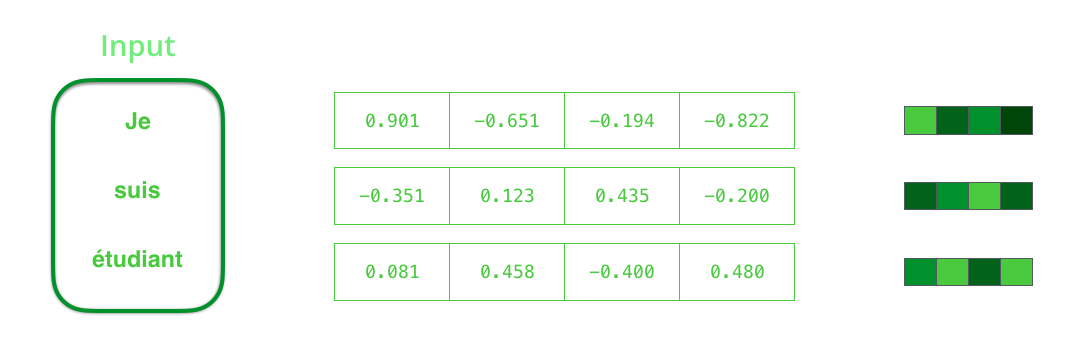
\includegraphics[width=0.65\textwidth]{example_word_embedding.png}
\vspace{-10pt}
\caption{\footnotesize Example Word Embeddings. From \emph{Visualizing Neural Machine Translation Mechanics of Seq2Seq Models with Attention}, by Jay Alammar, 2018. \url{http://jalammar.github.io/visualizing-neural-machine-translation-mechanics-of-seq2seq-models-with-attention/}. Copyright 2018 by Jay Alammar.}
\vspace{-10pt}
\label{fig:exampleWordEmb}
\end{figure}

According to Rudolph et al. (2016), ``each term in a vocabulary is associated with two latent vectors, an \emph{embedding} and a \emph{context vector}. These two types of vectors govern conditional probabilities that relate each word to its surrounding context." 
Rudolph and Blei (2017) note that a word embedding uses vector representations to parameterize the conditional probabilities of words in a surrounding context. 
In other words, a word's conditional probability combines its \emph{embedding} and \emph{context vectors} of surrounding words, with different methods combining them differently. Subsequently, word embeddings are fitted to given text data by maximizing the conditional probabilities of observed text (Rudolph et al. 2017). 

\subsection{Static Embeddings vs. Contextual Embeddings} \label{sec:StaticVsContextualEmb}

\subsubsection{What is Polysemy?} \label{sec:Polysemy}

\textbf{Polysemy} means that a word can have multiple, distinct meanings. The \textbf{distributional hypothesis} in NLP states that meaning depends on context, and words occurring in the same contexts have similar meaning (Wiedemann et al. 2019). 

\subsubsection{The Problem With Context-Free, Static Embeddings} \label{sec:ProblemWithStaticEmbs}

Classic word vectors, also called \textbf{static embeddings}, represent words in a low-dimensional continuous space in a static way: this means each word has a single word vector representation regardless of its context (Ethayarajh, 2019). \nameref{sec:SkipGram} (Mikolov et al., 2013a) and \nameref{sec:Glove} (Pennington et al., 2014) are well-known algorithms for producing these ``context-independent representations," as Peters et al. (2018) calls them, due to the fact that their word embedding matrix, inputted to a neural network representation, is trained to use co-occurring information in text, rather than using dynamic computation offered by \hyperref[sec:LanguageModels]{language models} (Batista, 2018). Although still able to capture latent syntactic and semantic meaning by training over large corpora, static embeddings by definition create a single vector representation per word, so all senses of a polysemous word are collapsed within a single representation (Ethayarajh, 2019). This can significantly reduce model performance. For instance, the word ``plant" would have an embedding that is the ``average of its different contextual semantics relating to biology, placement, manufacturing, and power generation" (Neelakantan et al., 2015). 

\subsubsection{A Better Solution: Contextual Embeddings To Capture Polysemy} \label{sec:SolutionWithContextEmbs}

In the Annual Review of Linguistics, Lenci (2018) states that ``distributional semantics is a usage-based model of meaning, based on the assumption that the statistical distribution of linguistic items in context plays a key role in characterizing their semantic behavior".

Rudolph et al. (2016) states that ``each data point $i$ has a \emph{context} $c$, which is a set of indices of other data points." Context is also a modeling choice; in different domains, context can differ. In language, the data point is taken to be a word and the context is the sequence of surrounding words. In neural data, the data point is neuron activity at a specific time and context is surrounding neuron activity. In shopping data, the data point refers to a purchase and context can mean other items in a basket (Rudolph et al., 2016). 

A \textbf{contextual word embedding (CWE)} is usually obtained using a \hyperref[sec:BidirectionalLM]{bidirectional language model (biLM)} to capture contextual information using forward and backward history to incorporate surrounding phrases of the word (Antonio, 2019). Typically, a model uses an encoder to process input sequence and squeeze the information into a fixed-length context vector. While word vectors are ``lookup tables", contextual embeddings include type information and \hyperref[sec:NeuralLM]{neural network} parameters to ``contextualize" a word (Smith, 2019). 

Recent efforts to capture polysemy for word embeddings cast aside the idea of using a fixed word sense inventory. This allows contextual embeddings to ``not only create one vector representation for each [word] type in the vocabulary" but to also create separate vectors for each token in a surrounding context. Indeed, experiments show that contextual embeddings can capture word senses successfully (Wiedemann et al., 2019). Wiedemann concludes that this allows for a more realistic model of natural language; contextual embeddings have proven their superiority over static embeddings for many NLP tasks such as text classification (Zampieri et al., 2019) and sequence tagging (Akbig et al., 2018). Although contextualization models such as the \nameref{sec:Transformer}, \nameref{sec:BERT}, \nameref{sec:ELMo}, \nameref{sec:TransformerXL}, \nameref{sec:XLNet}, and \nameref{sec:ERNIE_2} differ widely, modeling ``sentence or context-level semantics together with word-level semantics proved to be a powerful innovation" in the NLP world (Wiedemann et al., 2019). 


% done
\section{Language Models} \label{sec:LanguageModels}

A language model takes a sequence of word vectors and outputs a sequence of predicted word vectors by learning a probability distribution over words in a vocabulary. In representation terms, the ``vector representation of a word depends on the context vector representation" (Ibrahim, 2019).

Many tasks such as \nameref{nlptask:machinetranslationMT}, spell correction, text summarization, \nameref{nlptask:questionansweringQA}, and \nameref{nlptask:sentimentanalysisSA} all use language models to convert text into machine-interpretable language (Chromiak, 2017). 

Intuitively, language models predict words in a blank. For instance, given the following context: ``The $\_\_\_$ sat on the mat" where $\_\_\_$ is the word to predict, a language model might suggest the word ``cat" should fill the blank a certain percentage of the time and the word ``dog" would fill the blank with lower probability (Kurita, 2019). 

Formally, language models work by computing the conditional probability of a word $w_t$ given a context, such as its previous $n-1$ words, where the probability is: $P(w_t | w_{t-1}, ..., w_{t-n+1})$ (Ruder, 2016). Chromiak adds that the probability chain rule is the main tool used to find the joint probability of a word sequence. For events A and B, the probability chain rule states:
$$
P(A | B) = \frac{P(A \cap B)} {P(B)}
$$
which lends the following formula for a set of $T$ word tokens $w_1, ..., w_T$ from a sentence $S$: 
$$
\begin{array}{ll}
P(S)
&= P \Big(w_1, ..., w_T \Big)  \\
&= P(w_1) \cdot P(w_2 \; | \; w_1) \cdot ... \cdot P(w_n \; | \; w_1, ..., w_{T-1}) \\
&= \prod_{t=1}^T P \Big(w_t \; | \; w_1, ..., w_{t-1} \Big) \\
\end{array}
$$
Typically, the \textbf{Markov Assumption}, which states that the probability of a word depends only on its previous word, is used to reduce context history and thus intake of model data. Thus the joint probability is estimated using the $n$ previous words of the current word $w_t$:
$$
P \Big(w_1, ..., w_T \Big) \approx \prod_{t=1}^T P \Big(w_t \; | \; w_{t-1}, ..., w_{t-n+1} \Big)
$$

There are several kinds of language models. 

\subsection{N-gram Language Model} \label{sec:NGramLM}

An $n$-gram is a sequence of $n$ words. The $n$-gram language model is one of the simplest models that assigns probabilities to sentences and word sequences. It calculates a word's probability based on the frequencies of its constituent $n$-grams, taking just the preceding $n-1$ words as context instead of the entire corpus (Ruder, 2016): 
$$
P \Big(w_t \; | \; w_{t-1}, ..., w_{t-n+1} \Big) = \frac {count(w_{t-n+1},...,w_{t-1},w_t)} {count(w_{t-n+1},...,w_{t-1})}
$$

\subsection{Neural Network Language Model} \label{sec:NeuralLM}

\subsubsection{Curse of Dimensionality} \label{sec:CurseDim}

Bengio et al. (2003) defines the \emph{curse of dimensionality} in NLP as how a word sequence may differ from the training set of word sequences. This appears when modeling the joint distribution between discrete random variables (like words in a sentence). 

\subsubsection{Key Concept: Neural Network Representation} \label{sec:NeuralNetRepr}

A \textbf{neural network} is a function from vectors to vectors.  

All neural network representations rely on a structure called a neuron, which is expressed as a linear formula: $W \cdot x + b$. By applying a nonlinear function $f(\cdot)$ to this equation and by incorporating many hidden layers and by stacking neurons together, a neural network can model any function. A neuron is shown in \cref{fig:neuron}.

\begin{figure}[h]
\vspace{-5pt}
\centering
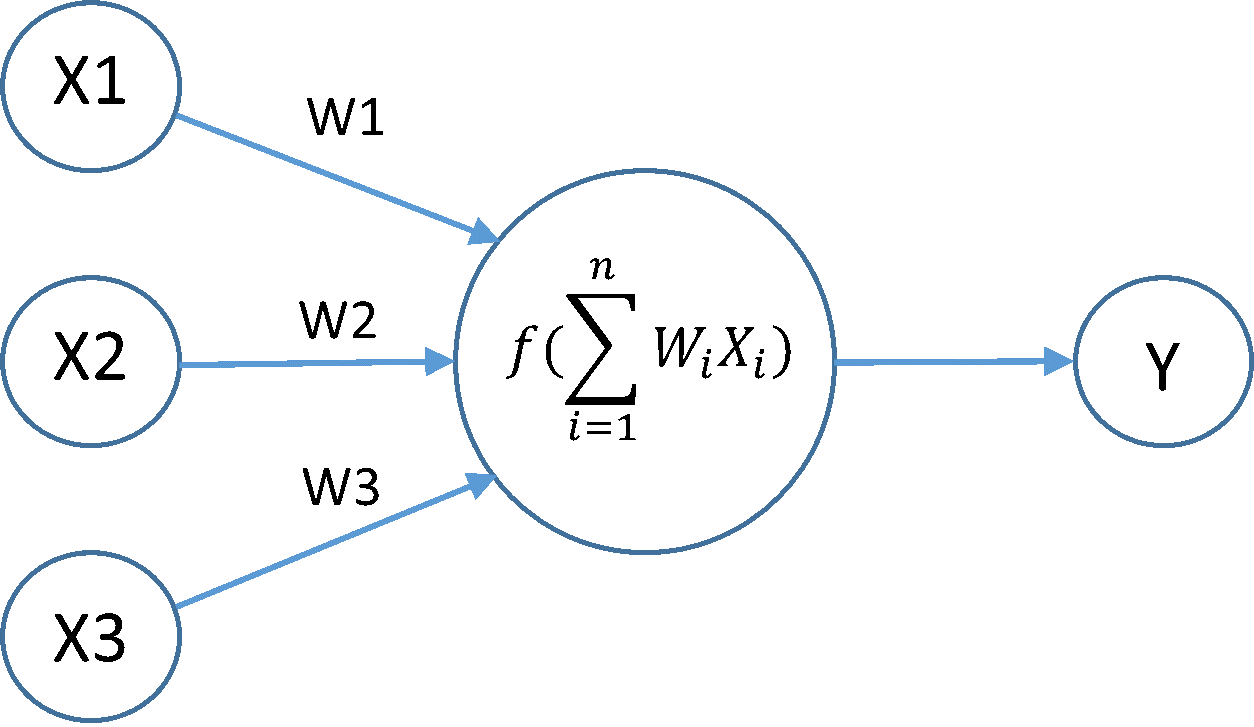
\includegraphics[width=0.35\textwidth]{neuron.png}
\vspace{-5pt}
\caption{\footnotesize Neuron. From \emph{Applying Unsupervised Machine Learning to Sequence Labeling}, by Jacob, 2019. \url{https://medium.com/mosaix/deep-text-representation-for-sequence-labeling-2f2e605ed9d}. Copyright n.d. by n.d.}
\vspace{-5pt}
\label{fig:neuron}
\end{figure}

Many \hyperref[app:Appendix_NLPTasks]{NLP applications} using neural networks feed in word tokens that is transformed based on its context words, resulting in an updated version of the word embedding (Smith, 2019). Embeddings are fed as parameters or weights into a neural network which \emph{optimizes} them to best fit the text by minimizing a continuous loss function using gradient-descent based algorithms. Every neural network representation consists of three components (Ruder, 2016):

\begin{enumerate}
    \item \textbf{Embedding Layer}\label{cnc:embeddingLayer}: this layer creates word embeddings by multiplying an index vector with a word vector matrix. 
    
    \item \textbf{Intermediate Layer(s)}: multiple layers are used to create a fully-connected layer that applies a non-linearity function (like hyperbolic tangent or sigmoid) to the concatenation of word embeddings. 
    
    \item \textbf{Softmax Layer}\label{cnc:softmaxLayer}: the last layer normalizes the word embedding matrix to using a \textbf{softmax function} to create a probability distribution over words $w_t$ in the vocabulary. 
    $$
    P \Big(w_t \; | \; w_{t-1}, ..., w_{t-n+1} \Big) = \frac {\exp{ \Big(h^T \cdot v_{w_t}' \Big) }} {\sum_{w_i \in V} \exp{ \Big(h^T \cdot v_{w_i}' \Big) }}
    $$
    where $V = $ vocabulary of a corpus, $h = $ output vector of the hidden layer, and $v_w' = $ the output embedding of word $w$. 
\end{enumerate}

Many neural networks are \textbf{feed-forward neural network (FNN)}\label{cnc:ffn}s, in which input is fed in the forward direction only. 


\subsubsection{Solution to Curse of Dimensionality: Neural Model and Continuous Vector Representations} \label{sec:SolutionToCurseDim}

The $n$-gram model seeks to remedy the \emph{curse of dimensionality} by combining short overlapping word sequences seen in the training set. 

However, Bengio et al. (2003) developed a \emph{neural probabilistic language model} to learn a \hyperref[sec:DistributedRepr]{distributed representation} for words to allow the model to generalize to unseen data. The neural model does two tasks simultaneously; (1) it learns a \hyperref[sec:DistributedRepr]{distributed representation} for each word, and also (2) it learns the probability distribution of word sequences \emph{as a function of} the \hyperref[sec:DistributedRepr]{distributed representations}. The model generalizes to unseen data successfully because unseen word sequences get a high probability if containing words that are similar to words that were already seen.  

Advantageously, this model can capture longer contexts better than the \hyperref[sec:NGramLM]{$n$-gram}, which is limited to short contexts. As a result of continuous word vector representations, the learned probability function's parameters increase linearly not exponentially with the vocabulary size, and they increase linearly with vector dimension, thus resolving the curse of dimensionality (Bengio et al., 2003).  

For more information, \nameref{app:Appendix_Backprop} mathematically explains how neural networks learn parameters. 


\subsection{Bidirectional Language Model} \label{sec:BidirectionalLM}

\subsubsection{Forward Language Model} \label{sec:ForwardLM}

A general language model predicts a next word given its context words, $P(\textit{Word} \: | \: \textit{Context})$. 

A \textbf{forward language model} takes this context to be previous words. From Peters et al. (2018), given a sequence of $N$ tokens $(t_1, t_2, ..., t_N)$, a forward language model calculates the probability of the tokenized sentence assuming the probability of a word token $t_k$ is conditional on its history tokens, $(t_1, ..., t_{k-1})$:
$$
P \Big(t_1, t_2, ..., t_N \Big) = \prod_{k=1}^N P \Big(t_k \; | \; t_1, t_2, ..., t_{k-1} \Big)
$$

\subsubsection{Backward Language Model} \label{sec:BackwardLM}

A \textbf{backward language model} is similar to a forward model excepts it predicts the current token $t_k$ conditional on future context tokens:
$$
P \Big(t_1, t_2, ..., t_N \Big) = \prod_{k=1}^N P \Big(t_k \; | \; t_{k+1}, t_{k+2}, ..., t_N \Big)
$$

\subsubsection{Combining Forward and Backward}

A \textbf{bidirectional language model (biLM)} such as in \cref{fig:bidirectionalLM} combines the \hyperref[sec:ForwardLM]{forward} and \hyperref[sec:BackwardLM]{backward language model}s and uses maximum likelihood estimation to \emph{jointly} maximize the log likelihood of the forward and backward directions: 
$$
\sum_{k=1}^N \Big( \text{log} \Big( P \Big(t_k \; | \; t_1,...,t_{k-1}; \; \overrightarrow{\theta} \Big) + \text{log} \Big( P \Big(t_k \; | \; t_{k+1}, t_{k+2}, ..., t_N; \; \overrightarrow{\theta} \Big) \Big)
$$
where $\overrightarrow{\theta}$ represents additional parameters (Peters et al., 2018). 


\begin{figure}[h]
\vspace{-5pt}
\centering
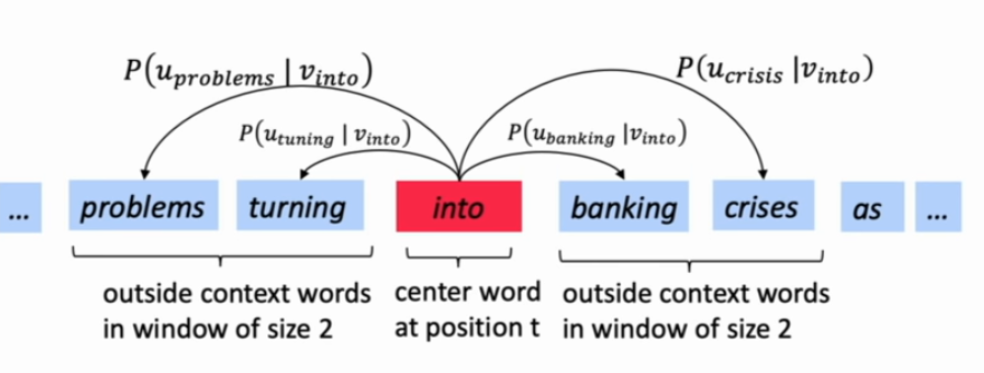
\includegraphics[width=0.6\textwidth]{bidirectional_languagemodel_banking.png}
\vspace{-5pt}
\caption{\footnotesize Example Bidirectional Language Model. From \emph{Word2Vec Overview With Vectors}, by CS224n: Natural Language Processing with Deep Learning (Stanford), 2018. \url{https://sangminwoo.github.io/2019-08-28-cs224n-lec1/}. Copyright n.d. by n.d.}
\vspace{-5pt}
\label{fig:bidirectionalLM}
\end{figure}

Akbik et al. (2018) use the hidden states of a bidirectional recurrent neural network to create contextualized word representations. 

For example, consider the sentences ``Mary accessed the bank account" and ``The swan waded to the bank of the river." In the first sentence, a unidirectional contextual model would represent the target word ``bank" based on `I accessed the' but not `account,' thus failing to capture the polysemy of `bank.' But a bidirectional language model represents ``bank" using both previous and next context to ameliorate this problem.
% done
\section{Word2Vec} \label{sec:Word2Vec}

% \subsection{Word Embedding Representations: Count-Based vs. Context-Based} \label{sec:CountVsContextModels}
 
%Word embeddings can be learned using two kinds of contextual vector space models: the \textbf{count-based} or \textbf{context-based vector space models}. 

%\textbf{Count-based vector space models} are unsupervised learning algorithms based on matrix factorization of a global word co-occurrence matrix. The main assumption is words in similar contexts share related semantic meanings. Examples include PCA and neural probabilistic language models. Another term for this type is \textbf{distributed semantic model} (DSM) (Weng, 2017). 

%\textbf{Context-based vector space models} are supervised algorithms that use a local context to predict target words. These are predictive models which take dense word vectors as parameters and update word representations during training.

%In 2014, Baroni et al. showed that predictive approaches outperformed count models significantly and consistently. 

%Although \textbf{Word2Vec} and \nameref{sec:Glove} are predictive and context-based vector space models, they still rely on co-occurrence counts. 

\subsection{Motivation for Word2Vec}

\textbf{Word2Vec} is an unsupervised learning algorithm for obtaining word vector representations using a two-layer neural network. Existing word representations already capture linguistic patterns, allowing algebraic operations to be done on the word vectors in their semantic vector space. But Mikolov et al. (2013b) created \textbf{Word2Vec} to learn \emph{efficient} representations from \emph{large} data, as opposed to previous architectures that reduced quality of learned vectors by using smaller data and dimensionality. 


Both the \nameref{sec:SkipGram} and \nameref{sec:CBOW} in Word2Vec are \hyperref[sec:NeuralLM]{neural network language models} with one hidden layer.  Their input vector $\overrightarrow{x} = (x_1,..., x_V)$ and output vector $\overrightarrow{y} = (y_1,...,y_V)$ are both \textbf{\hyperref[sec:OneHotEncodings]{one-hot encodings}}, and the hidden layer of the \hyperref[sec:NeuralLM]{neural network} is a \hyperref[sec:WordEmbeddings]{word embedding} with dimension $N$. 

\subsubsection{Key Concept: One-Hot Encodings} \label{sec:OneHotEncodings}

A \textbf{one-hot vector encoding} is the simplest type of word embedding where each cell in the vector corresponds to a distinct vocabulary word. A $1$ is placed in the cell marking the position of the word in the vocabulary, and $0$ elsewhere. A problem with these is they lead to high-dimensional vectors for large vocabularies, raising computational costs. Secondly, they do not let similarity between words to be represented. 

%(Thus even though the vocabulary size is $V$, the goal is to learn embeddings with size $N$). 
%For time $t$, Word2Vec predicts one output word $w_{t+j}$ (vector $\overrightarrow{y}$) given one input word $w_t$ (vector $\overrightarrow{x}$). For \textbf{Skip-Gram}, $w_{t+j}$ is the predicted context word and $w_t$ is the input target word, but for \textbf{CBOW} $w_{t+j}$ is the predicted target word and $w_t$ is the input context word.   

%Vectors $v_w$ and $v'_w$ are two representations of word $w$. Vector $v_w$ comes from the rows of the \textit{input layer $\rightarrow$ hidden layer weight matrix} $W$, and vector $v'_w$ comes from the rows of the \textit{hidden layer $\rightarrow$ output layer weight matrix} $W'$. We call $v_w$ the \textbf{input vector} and $v'_w$ is the \textbf{output vector} of the word $w$. 


\subsubsection{Skip-Gram} \label{sec:SkipGram}

The Skip-Gram model predicts context words given a single target word. It uses a fixed sliding window to capture bidirectional context along a sentence, around a single target word. The target is input as a one-hot encoding to a neural network which updates the target vector with values near $1$ in cells corresponding to predicted context words (Weng, 2017).  The Skip-Gram is illustrated in \cref{fig:SkipGram}.

Consider the following sentence from Weng (2017): ``The man who passes the sentence should swing the sword." Using context window size $c = 5$ and target word ``swing", the Skip-Gram should learn to predict the context words $\{$\texttt{"sentence"}, \texttt{"should"}, \texttt{"the"}, \texttt{"sword"} $\}$, and so the target-context word pairs fed into the model for training are: (\texttt{"swing"}, \texttt{"sentence"}), (\texttt{"swing"}, \texttt{"should"}), (\texttt{"swing"}, \texttt{"the"}), and (\texttt{"swing"}, \texttt{"sword"}).  



\begin{figure}
\centering
\begin{minipage}{.48\textwidth}
  \centering
  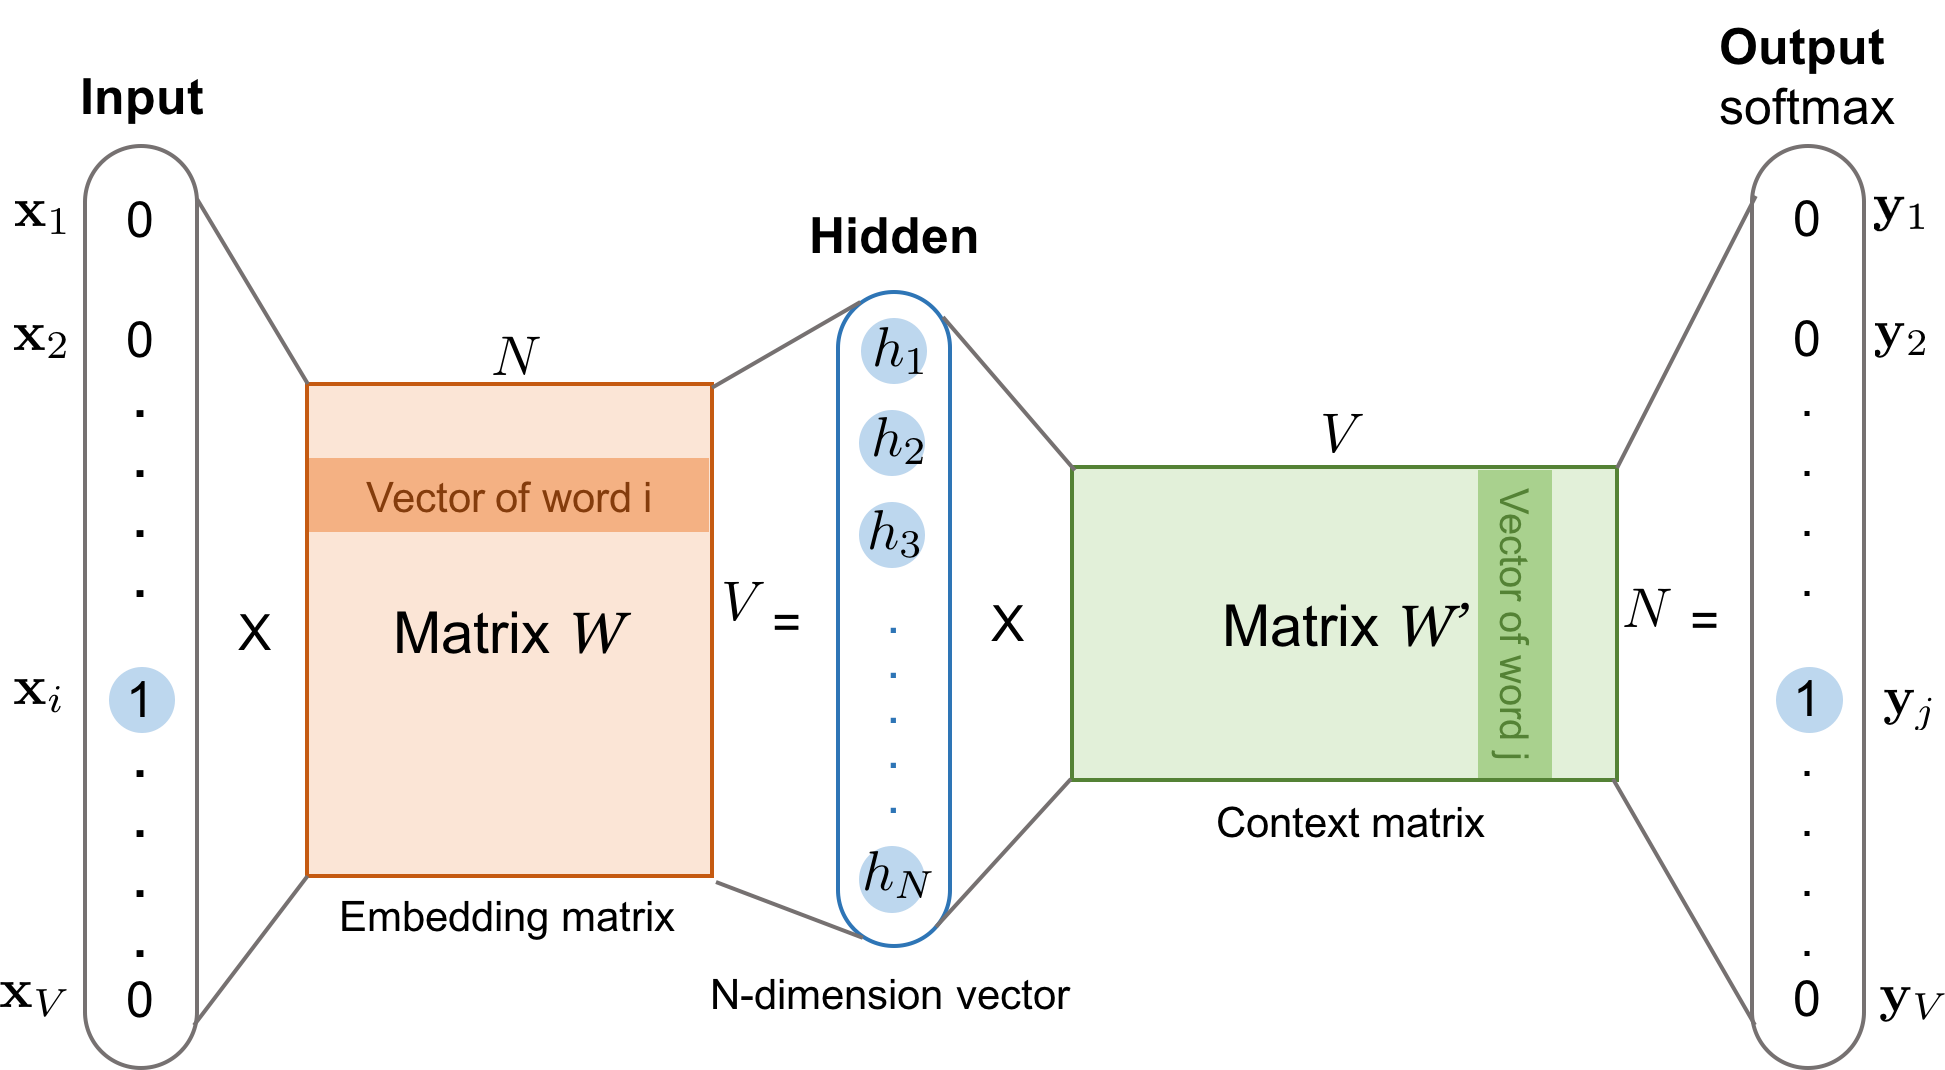
\includegraphics[width=\textwidth]{imgs/skipgram_image.png}
  \captionof{figure}{Simplified Skip-Gram Model with one input target word and one output context word. From \emph{Learning Word Embeddings}, by Lilian Weng, 2017. \url{https://lilianweng.github.io/lil-log/2017/10/15/learning-word-embedding.html}. Copyright 2017 by Weng.}
  \label{fig:SkipGram}
\end{minipage} \hspace{1.5em}%
\begin{minipage}{.48\textwidth}
  \centering
  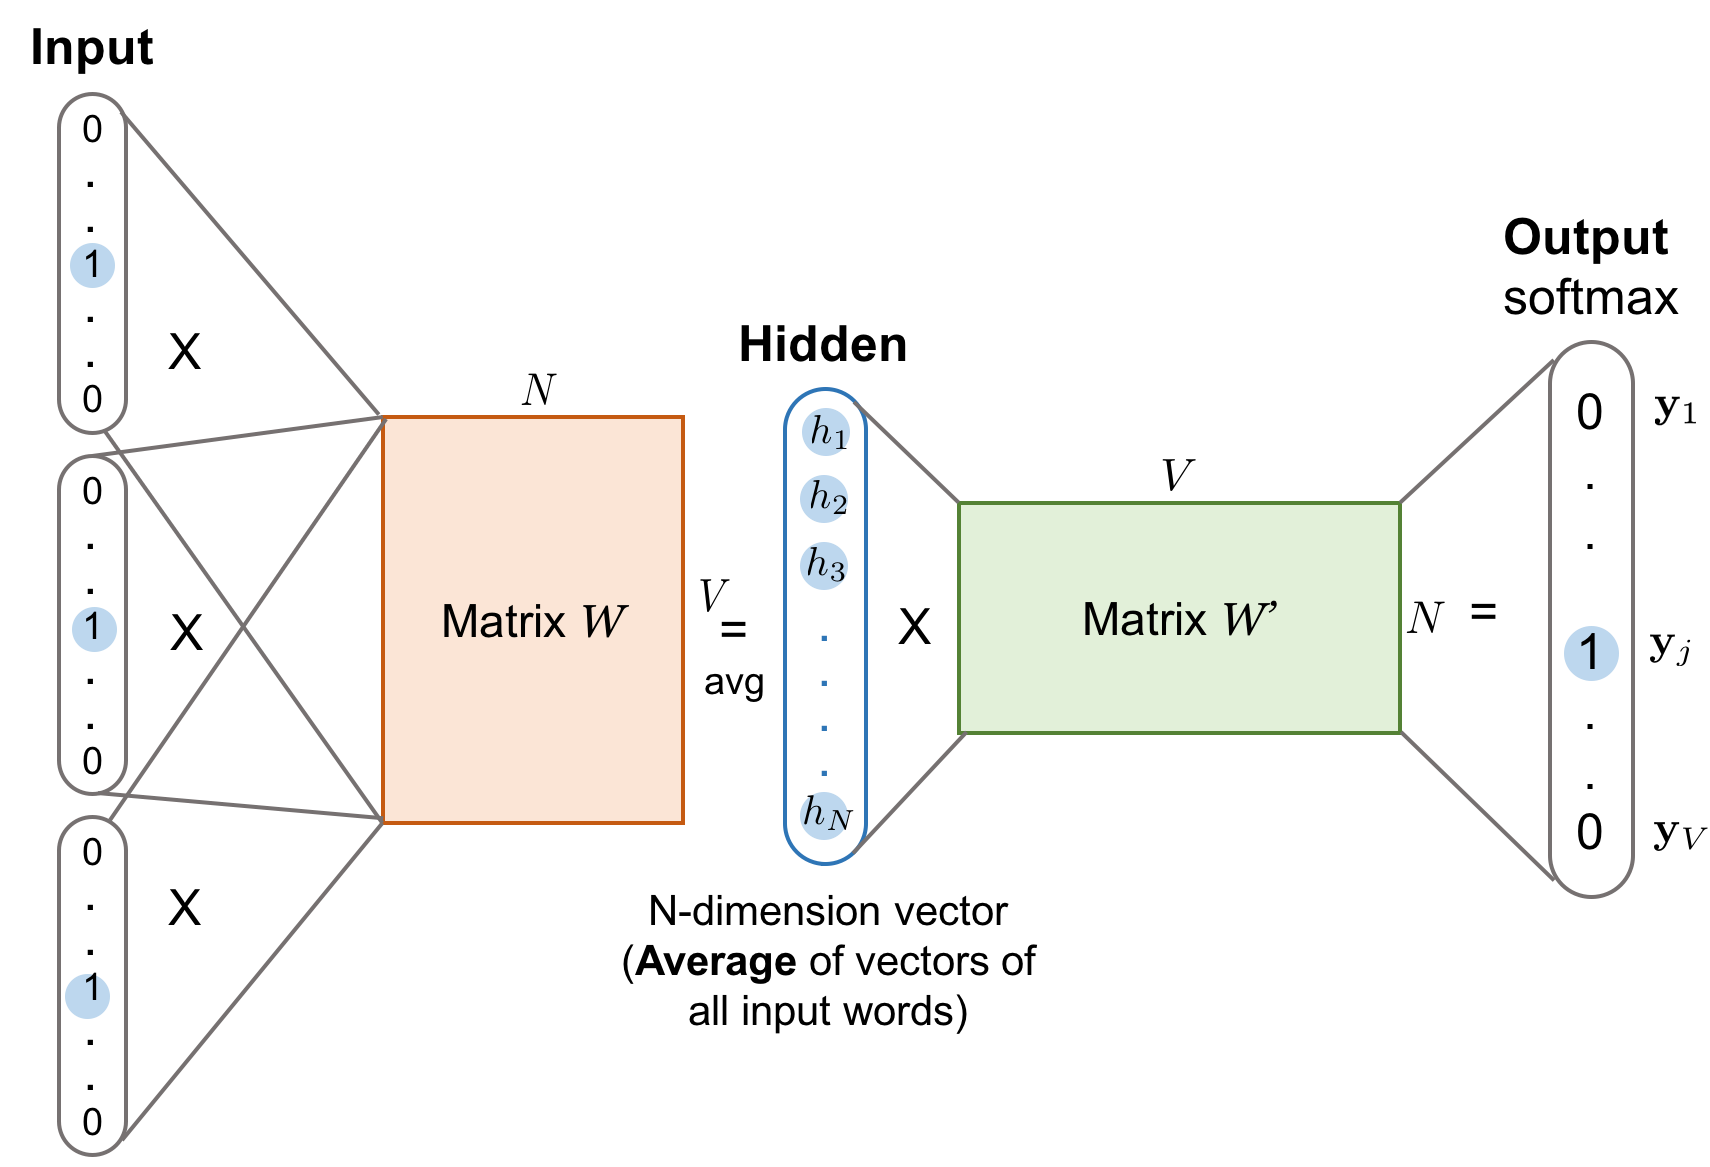
\includegraphics[width=\textwidth]{imgs/cbow.png}
  \captionof{figure}{CBOW Model with several one-hot encoded context words at the input layer and one target word at the output layer. From \emph{Learning Word Embeddings}, by Lilian Weng, 2017. \url{https://lilianweng.github.io/lil-log/2017/10/15/learning-word-embedding.html}. Copyright 2017 by Weng.}
  \label{fig:CBOW}
\end{minipage}
\end{figure}


% 
% \subsubsection{Forward and Backward Pass for Skip-Gram}
% 
% According to the Skip-Gram illustrated in \cref{fig:SkipGram}, the procedure for learning word vectors is: 
% \begin{enumerateSpaced}{3pt}
%     \item the input word $w_i$ and output word $w_j$ are encoded as one-hot vectors, $\overrightarrow{x}$ and $\overrightarrow{y}$ respectively. (For Skip-Gram, $\overrightarrow{x}$ is the target vector and $\overrightarrow{y}$ is the context vector). 
%     
%     \item A randomly initialized word embedding matrix $W$ with size $V \times N$ at the input $\rightarrow$ hidden layer is multiplied with $\overrightarrow{x}$ to give the $N$-dimensional embedding for target word $w_i$. This embedding resides in the $i$-th row of $W$ and is considered as the hidden layer of the model. 
%     
%     \item Next, the hidden layer is multiplied by weight matrix $W'$ with size $N \times V$ to produce the one-hot encoded output vector, $\overrightarrow{y}$. \textbf{NOTE: }the output context matrix $W'$ encodes words as context and is distinct from the embedding matrix $W$. 
%     
%     \item The result of the above multiplication is sent through the softmax layer to create a probability distribution over the words. The above steps constitute the \hyperref[sec:ForwardProp]{forward pass}.
%     
%     \item \hyperref[sec:ErrorCalc]{Errors} are obtained by subtracting the output vector with the target vector. 
%     
%     \item The error vector is \hyperref[sec:BackwardProp]{backward-propagated} through the neural network to update the weight matrix. The procedure continues until errors are small enough. 
%     
% \end{enumerateSpaced}
% 




\subsubsection{Continuous Bag of Words Model (CBOW)} \label{sec:CBOW}

The \textbf{continuous bag of words model (CBOW)} is opposite to Skip-Gram since it predicts the \emph{target} word based on a \emph{context} word. Generally during training, CBOW receives a window of $n$ context words around the target word $w_t$ at each time step $t$ to predict the target word (Mikolov et al., 2013b). The forward pass for CBOW is similar to Skip-Gram's, except CBOW averages context word vectors while multiplying INPUT $\overrightarrow{x}$ and the \emph{input} $\rightarrow$ \emph{hidden layer} matrix $W$. From Rong (2016), $\overrightarrow{h} = \frac{1}{c} W \cdot \Big(\overrightarrow{x_1} + \overrightarrow{x_2} + ... + \overrightarrow{x_c} \Big) = \frac{1}{c} \cdot \Big(\overrightarrow{v_{w_1}} + \overrightarrow{v_{w_2}} + ... + \overrightarrow{v_{w_c}} \Big)$, where $c$ is the number of context words, $w_1,...,w_c$ are the context words, and $v_w$ is the input vector for general word $w$. According to Weng (2016), the fact that CBOW averages distributional information of the context vectors makes CBOW better suited for small datasets. The CBOW is shown in \cref{fig:CBOW}.


\subsection{Phrase-Learning in Word2Vec Using Skip-Gram}

The problem with previous word vectors is their lack of phrase representation. ``Canada" and ``Air" could not be recognized as part of a larger concept and be combined into ``Air Canada". Many phrases have meaning that is not just a composition of the meanings of its individual words and should be represented as a unique identity. In contrast, a bigram like ``this is" should remain unchanged (Mikolov et al., 2013a, p. 5). 

As an attempt to solve this, the \textbf{Phrase Skip-Gram} forms phrases based on the score $S_{phrase} = \frac{C(w_i w_j) - \delta} {C(w_i)C(w_j)}$, where $C(\cdot)$ is the count of a unigram $w_i$ or bigram $w_i w_j$ and $\delta$ is a discounting threshold to avoid creating infrequent words and phrases. High values of $S_{phrase}$ means the phrase is most likely a phrase rather than simple concatenation of two words. Mikolov et al. (2013a) found that this Phrase Skip-Gram with hierarchical softmax and subsampling outperformed the original model on large data. 

Also, the Phrase Skip-Gram creates vectors exhibiting a linear structure called \textbf{additive compositionality}, which allows words to be combined meaningfully by adding their word vectors. Since learned context vectors can represent the overall distribution of context words in which the target word appears, and since the vectors in the loss function are logarithmically related to the probabilities from the output layer, the sum of two word vectors is related to the product of the context distributions (using the logarithm sum rule). This product of distributions acts like an AND function since words are weighted by probability. Consequently, if the key phrase ``Volga River" appears many times in the same sentence along with ``Russian" and ``river", the sum $vector(\texttt{"Russian"}) \! + \! vector(\texttt{"river"})$ results in the phrase $vector(\texttt{"Volga River"})$ or at least a vector close to it (Mikolov et al., 2013a). 
% done
\section{GloVe} \label{sec:Glove}

The \textbf{Global Vectors for Word Representation (GloVe)} model is an unsupervised learning algorithm that aims to capture meaning in a semantic vector space using global count statistics instead of local context (Pennington et al., 2014). GloVe uses probability ratios to represent meaning as vector offsets. 



\subsection{Problem with Word2Vec: Secret in the Loss Function} \label{sec:ProblemWord2VecFromGloveStandpoint}

\nameref{sec:Word2Vec} uses only local and not global context. So even though words ``the" and ``cat" might be used together frequently, \nameref{sec:Word2Vec} will not discern if this is because ``the" is a common word or because ``the" and ``cat" are actually correlated (Kurita, 2018). 

From Pennington et al. (2014), \nameref{sec:Word2Vec} implicitly optimizes over a co-occurrence matrix while streaming over input sentences. In doing so, it optimizes its log likelihood loss of seeing words \emph{simultaneously} in the same context windows, resulting in an alternative way in \cref{eq:Word2VecLossFunction} of expressing \nameref{sec:Word2Vec}'s loss function. 

\begin{equation} 
J = - \sum_i X_i \sum_j P_{ij} \text{log}(Q_{ij}) 
\label{eq:Word2VecLossFunction}
\end{equation} 

In \cref{eq:Word2VecLossFunction}, $X_i = \sum_k X_{ik}$ is the total number of words appearing in the context of word $i$ and $Q_{ij}$ is the probability that word $j$ appears in context of word $i$ and is estimated as $Q_{ij} = \text{softmax} \Big( w_i \cdot w_j \Big)$. Evidently, \nameref{sec:Word2Vec}'s loss function is form of cross entropy between the predicted and actual word distributions found in context of word $i$. The problem with this is twofold: (1) cross entropy models long-tailed distributions poorly, and (2) the cross-entropy here is weighted by $X_i$, causing equal-streaming over data, so a word appearing $n$ times contributes to the loss $n$ times (Pennington et al., 2014). Recognizing there is no inherent justification for streaming across all words equally, GloVe instead computes differences between unnormalized probabilities, contrary to \nameref{sec:Word2Vec} (Kurita, 2018a). 


\subsection{Motivation for GloVe} \label{sec:MotivationGlove}

Previous global count models like Latent Semantic Analysis (LSA) produced word embeddings lacking vector analogical properties and lacking \emph{dimensions of meaning} such as gender, grammar tense, and plurality, disabling downstream models from easily extracting meaning from those word vectors (Kurita, 2018a). Building from past failures while avoiding \nameref{sec:Word2Vec}'s local \hyperref[sec:ProblemWord2VecFromGloveStandpoint]{context problems}, GloVe instead uses a principled and explicit approach for learning these \emph{dimensions of meaning}.


\subsection{Describing GloVe} \label{sec:DefGlove}

%\subsubsection{Notation in GloVe}

%Let $X$ be the matrix of word co-occurrence counts; let $X_{ij}$ be the $ij$-th entry $X$ that counts how many times any word appears in the context of word $i$, and let $P_{ij} = p_{\text{co}} \Big(w_j \; | \; w_i \Big) = \frac {X_{ij}} {X_i}$ be the probability that word $j$ appears in the context of word $i$ (Pennington et al., 2014; Weng, 2017).

\subsubsection{Meaning Extraction Using Co-Occurrence Counts}

GloVe uses a co-occurrence matrix that describes how words co-occur within a fixed sliding window, assuming co-occurrence counts reveal word meaning. Words \textbf{co-occur} when they appear together within this fixed window (Kurita, 2018a). GloVe takes the matrix as input, rather than the entire corpus, so GloVe disregards sentence-level information while taking into account only corpus-wide co-occurrence. 

From Weng (2017), the co-occurrence probability is defined as: 
$$
p_{\text{co}} \Big(w_k \; | \; w_i \Big) = \frac{C(w_i, w_k)}{C(w_i)}
$$
where $C(w_i, w_k)$ counts the co-occurrence between words $w_i$ and $w_k$.  

GloVe's insight is that word meanings are captured by ratios of co-occurrence probabilities rather than the probabilities themselves. To illustrate how GloVe uses these counts, consider two words $w_i =$ ``ice" and $w_j = $ ``steam". 

\begin{itemizeSpaced}{0pt}
    \item \textbf{Case 1:} For context words related to \texttt{ice} but not \texttt{steam} (like \texttt{solid}), the co-occurrence probability $p_{\text{co}} \Big( \texttt{solid} \; | \; \texttt{ice} \Big)$ should be much larger than $p_{\text{co}} \Big( \texttt{solid} \; | \; \texttt{steam} \Big)$, therefore the ratio $\frac {p_{\text{co}} \Big( \texttt{solid} \; | \; \texttt{ice} \Big)} {p_{\text{co}} \Big( \texttt{solid} \; | \; \texttt{steam} \Big)}$ gets very large.

    \item \textbf{Case 2: } Conversely, for words related to \texttt{steam} but not \texttt{ice} (like \texttt{gas}) $\Rightarrow$ the co-occurrence ratio $\frac {p_{\text{co}} \Big( \texttt{gas} \; | \; \texttt{ice} \Big)} {p_{\text{co}} \Big( \texttt{gas} \; | \; \texttt{steam} \Big)}$ should be small. 

    \item \textbf{Case 3:} For words $w$ related to both \texttt{ice} and \texttt{steam} (like \texttt{water}) or related to neither (like \texttt{fashion}), the ratio $\frac {p_{\text{co}} \Big( w \; | \; \texttt{ice} \Big)} {p_{\text{co}} \Big( w \; | \; \texttt{steam} \Big)}$ should be near one. 
\end{itemizeSpaced}


% 
% \subsubsection{Comparing Performance of Word2Vec and GloVe}
% 
% \cref{fig:gloveVsWord2vec} from Pennington et al. (2014) shows that GloVe's learned word embeddings had higher prediction accuracy over both those of \nameref{sec:SkipGram} and \hyperref[sec:CBOW]{CBOW} (using negative sampling) on tasks like \nameref{nlptask:wordanalogy} and \nameref{nlptask:namedentityrecognitionNER}. 
% 
% \begin{figure}[h]
% \vspace{-5pt}
% \centering
% 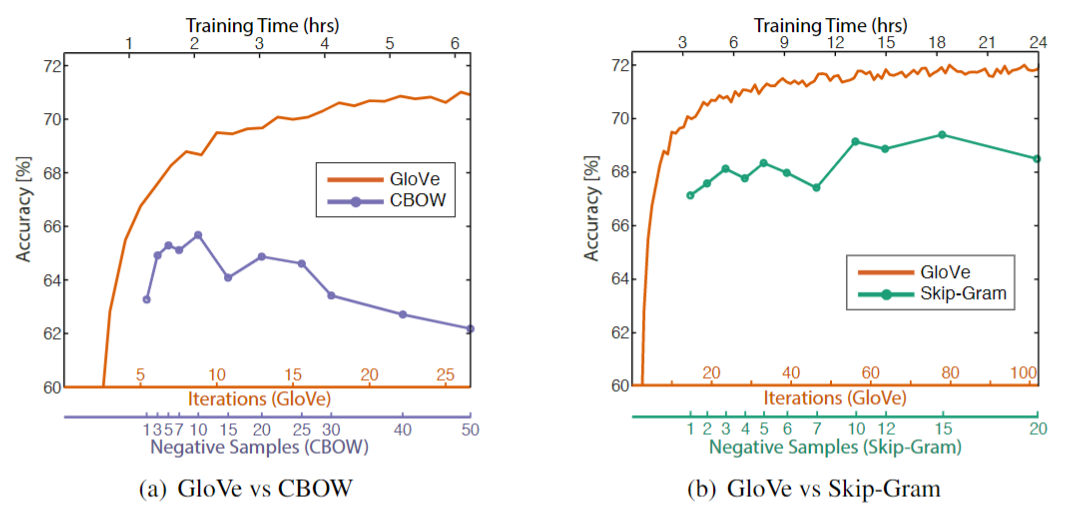
\includegraphics[width=0.65\textwidth]{imgs/table_gloveVSword2vec.png}
% \vspace{-5pt}
% \caption{Overall accuracy on word analogy task as a function of training time, which is governed by the number of iterations for \nameref{sec:Glove} and by the number of negative samples for \hyperref[sec:CBOW]{CBOW} (a) and \nameref{sec:SkipGram} (b). Pennington et al. (2014) train 300-dimensional vectors on the same 6B token corpus from Wikipedia and use a symmetric context window of size 10. From \emph{GloVe: Global Vectors for Word Representation}, by Pennington et al., 2014. \url{https://nlp.stanford.edu/pubs/glove.pdf}. Copyright 2014 by Pennington et al.}
% \vspace{-5pt}
% \label{fig:gloveVsWord2vec}
% \end{figure}% done
\section{Sequence To Sequence Model} \label{sec:Seq2Seq}

A \textbf{sequence-to-sequence (Seq-to-Seq) model} is often used in natural language processing for \nameref{nlptask:machinetranslationMT}. It takes a sequence of items such as words and outputs another sequence of items. It uses an \textbf{Encoder} that processes the inputs, squashes this information into a \emph{fixed-length} \textbf{context vector}, also known as a \textbf{sentence embedding} or \textbf{thought vector}. The Seq-to-Seq model sends this representation of the source sentence to a \textbf{Decoder} that outputs a target sentence one word at a time, using the context vector (Alammar, 2018a). Commonly, the Encoder and Decoder are \hyperref[sec:RNN]{RNNs} such as \hyperref[sec:LSTM]{LSTMs} or \hyperref[sec:GRU]{GRUs}.


\subsection{Describing Seq-to-Seq Model}

The key feature in the Seq-to-Seq model different from a \hyperref[sec:RNN]{recurrent neural network (RNN)} is the \textbf{context vector}, or the final hidden state of the Encoder. When the Encoder processes the input sequence $\overrightarrow{x} = \{ x_1, ..., x_{T_x} \}$ of individual word vectors $x_t$ in the input sentence $X$, the information is squashed into a \emph{fixed-length} context vector. Formally, a \hyperref[sec:GRU]{gated recurrent unit (GRU)} as the Encoder would output a hidden state given a previous hidden state and the current input: 
$$
h_t = \text{EncoderGRU} \Big( x_t, h_{t-1} \Big)
$$ 
where the context vector named $z$ equals the last hidden state: $z = h_{T_x}$. 
  
The context vector is then passed to the Decoder along with a target token $y_t$ and previous Decoder hidden state $s_{t-1}$ to return a current hidden state, $s_t$:
$$
s_t = \text{DecoderGRU} \Big( y_t, s_{t-1}, z \Big)
$$
The context vector $z$ does not have a time step $t$ subscript, meaning this same context vector from the Encoder is reused each time step in the Decoder. 


\begin{figure}[h]
\vspace{-5pt}
\centering
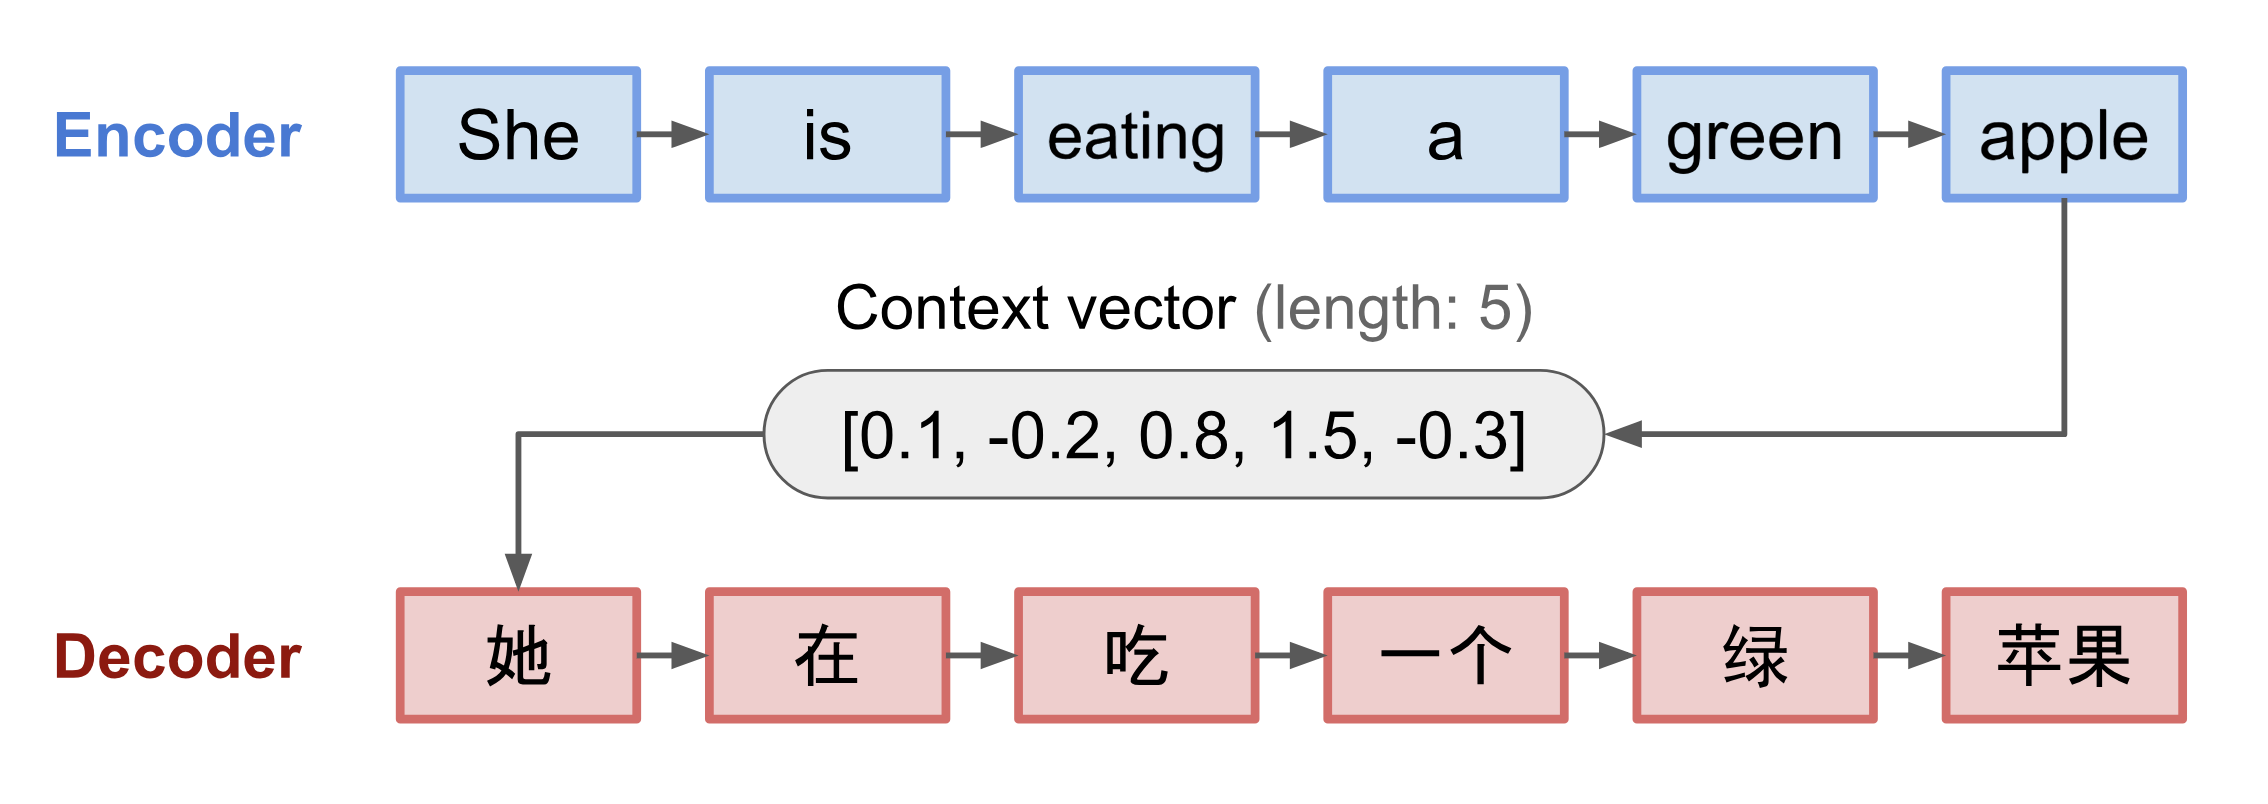
\includegraphics[width=0.6\textwidth]{imgs/seqtoseq_greenapple.png}
\vspace{-5pt}
\caption{\footnotesize Encoder-Decoder with Context Vector in a Seq-to-Seq model, translating the sentence ``She is eating a green apple" to Chinese. From \emph{Attention? Attention!}, by Weng, 2018. \url{https://lilianweng.github.io/lil-log/2018/06/24/attention-attention.html}. Copyright 2018 by Weng.}
\vspace{-5pt}
\end{figure}


\subsection{Problem with Seq-to-Seq Models} \label{sec:ProblemWithSeq2Seq}

Compressing the inputs into such a \textbf{fixed-length} vector leads to a \textbf{long-term dependency problem} since only the last hidden state of the Encoder is used. Thus, the Seq-to-Seq model becomes \textit{\hyperref[sec:ProblemWithRNNs]{incapable of memory}}, similar to  \hyperref[sec:RNN]{RNNs}.

\subsection{The Attention Mechanism} \label{sec:AttentionMechanism}

The \textbf{attention mechanism} was proposed in \nameref{nlptask:neuralmachinetranslationNMT} task to memorize longer sentences by ``selectively focusing on parts of the source sentence" as required (Luong et al., 2015). Instead of creating a single context vector $z$ from the Encoder's last hidden state $h_{T_x}$, the \emph{attention architecture} creates a context vector for each input word or timestep $t$, reducing the information compression problem. This means the attention mechanism uses all the hidden states generated by the Encoder as inputs for the decoding process. For each Decoder output, the attention mechanism ``selectively picks out specific elements from the [input] sequence to produce the [Decoder] output" (Loye, 2019). This essentially creates links between the context vector and entire source input. A general illustration is in \cref{fig:attention}.

\begin{figure}[h]
\centering
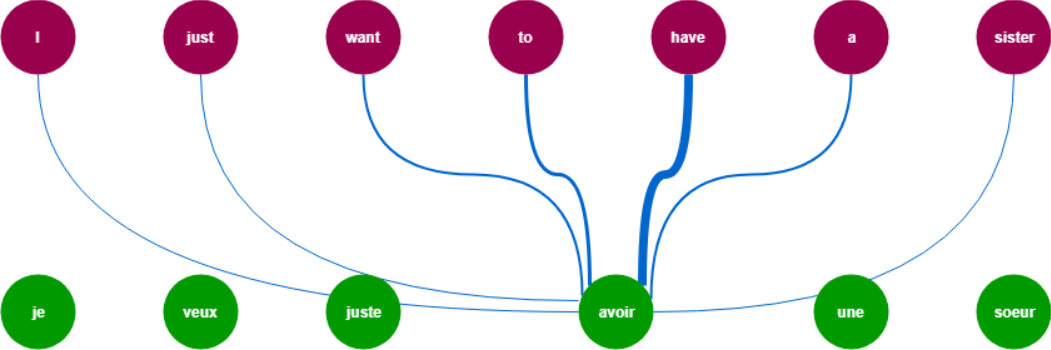
\includegraphics[width=0.6\textwidth]{imgs/attention.png}
\caption{\footnotesize Attention Mechanism: How words are considered for contextual evidence. From \emph{Intuitive Understanding of Seq2seq model and Attention Mechanism in Deep Learning}, by Medium, 2019. \url{https://medium.com/analytics-vidhya/intuitive-understanding-of-seq2seq-model-attention-mechanism-in-deep-learning-1c1c24aace1e}. Copyright n.d by n.d.}
\label{fig:attention}
\end{figure}

\subsection{Seq-to-Seq Model Using Attention}

The key components of a Seq-to-Seq model with attention are its attention \hyperref[sec:ForwardProp]{forward pass}, which computes attention scores, and Decoder \hyperref[sec:ForwardProp]{forward pass}, which outputs the context vector. 

\subsubsection{Forward Pass of Attention}

The attention mechanism is viewed as a layer in the Seq-to-Seq model with a \hyperref[sec:ForwardProp]{forward pass} that updates parameters. The steps for the \hyperref[sec:ForwardProp]{forward pass} to calculate attention scores $\alpha_{ti}$ is as follows: 
\begin{enumerate}
    \item First, an \textbf{alignment model} $\text{align}$ is used to calculate \textbf{energy scores} $e_{ti}$ that measure how well the ``inputs around position $i$ and the output at position $t$ match" (Bahdanau et al., 2016). The energy scores are weights specifying how much of the Decoder hidden state $s_{t-1}$ and the Encoder hidden state $h_i$ of the source sentence should be considered for each output (Ta-Chun, 2018; Bahdanau et al., 2016). 
    $$
    e_{ti} = \text{align} \Big(s_{t-1}, h_i \Big)
    $$ 
    
    \item Next, the energy score $e_{ti}$ is passed through a \hyperref[sec:NeuralLM]{feed-forward neural network} and \hyperref[cnc:softmaxLayer]{softmax} to calculate the attention scores, $\alpha_{ti}$:
    $$
    \alpha_{ti} = \frac{\exp{(e_{ti})} } { \sum_{k=1}^{T_x} \exp{(e_{ik})} }
    $$
    Transforming the energy scores via \hyperref[cnc:softmaxLayer]{softmax} ensures the attention vector $\overrightarrow{\alpha} = \Big \{ \alpha_{ti} \Big \}$ has values normalized between $0$ and $1$. 
\end{enumerate}

%\begin{center}
%    \pythonCodeFile{code/tut3_AttentionClass.py}
%\end{center}

% TODO: line wrapping

\subsubsection{Forward Pass of Decoder}

Once the attention scores have been calculated, the Decoder can calculate the context vector, $c_t$, which is a sum of Encoder hidden states $h_i$ weighted by attention scores $\overrightarrow{\alpha} = \Big \{ \alpha_{ti} \Big \}$ (Ta-Chun, 2018): 
$$
c_t = \sum_{i=1}^{T_x} \alpha_{ti} \cdot h_i
$$

Intuitively, the context vector is an \textbf{expectation}. The attention score $\alpha_{ti}$ is the probability that target word $y_t$ is aligned to (or translated from) an input word $x_j$. Then the $t$-th context vector $c_t$ is the expected hidden state over all hidden states $h_i$ with probabilities $\alpha_{ti}$, where these corresponding energies $e_{ti}$) quantify the importance of Encoder hidden state $h_i$ with respect to the previous Decoder hidden state $s_{t-1}$ in deciding the next Decoder state $s_t$ for generating target word $y_t$.   

Through this attention mechanism in the Decoder, we can relieve the Encoder of the burden of encoding all source sentence information into a fixed-length vector, allowing information to spread through the hidden state sequence $\overrightarrow{h} = \Big \{ h_1,...,h_T\Big \}$ and later be retrieved by the Decoder (Trevett, 2020).  

%\begin{center}
%    \pythonCodeFile{code/tut3_DecoderClass.py}
%\end{center}


\subsubsection{Forward Pass of Seq-to-Seq Model}

Finally, the Seq-to-Seq model can use the Encoder, Decoder and attention in conjunction. Its \hyperref[sec:ForwardProp]{forward pass} is (Trevett, 2020): 
\begin{enumerate}
    \item Create an output tensor to hold predicted words $\hat{y}$
    
    \item Pass the source sequence $\overrightarrow{x} = \Big \{ x_1, ..., x_T \Big \}$ into the Encoder to receive the contexts $\overrightarrow{z}$ alongside the hidden states $\overrightarrow{h} = \Big \{ h_1, ..., h_T \Big \}$.
    
    \item Set equal the initial Decoder hidden state $s_0$ and last Encoder hidden state $h_T$.
    
    \item Decode within a loop: insert the target token $y_t$ and previous hidden state $s_t$ and all Encoder outputs $\overrightarrow{h}$ into the Decoder to get a prediction $\hat{y}_{t+1}$ and new hidden state $s_t$.
    
    
\end{enumerate}

As an application of the Seq-to-Seq model with attention to \nameref{nlptask:neuralmachinetranslationNMT}, PyTorch code with explanations can be found in \nameref{app:Appendix_Seq2Seq}
%\begin{center}
%    \pythonCodeFile{code/tut3_Seq2Seq.py}
%\end{center}% done
\section{Transformer} \label{sec:Transformer}

\begin{figure}[h]
\vspace{-10pt}
\centering
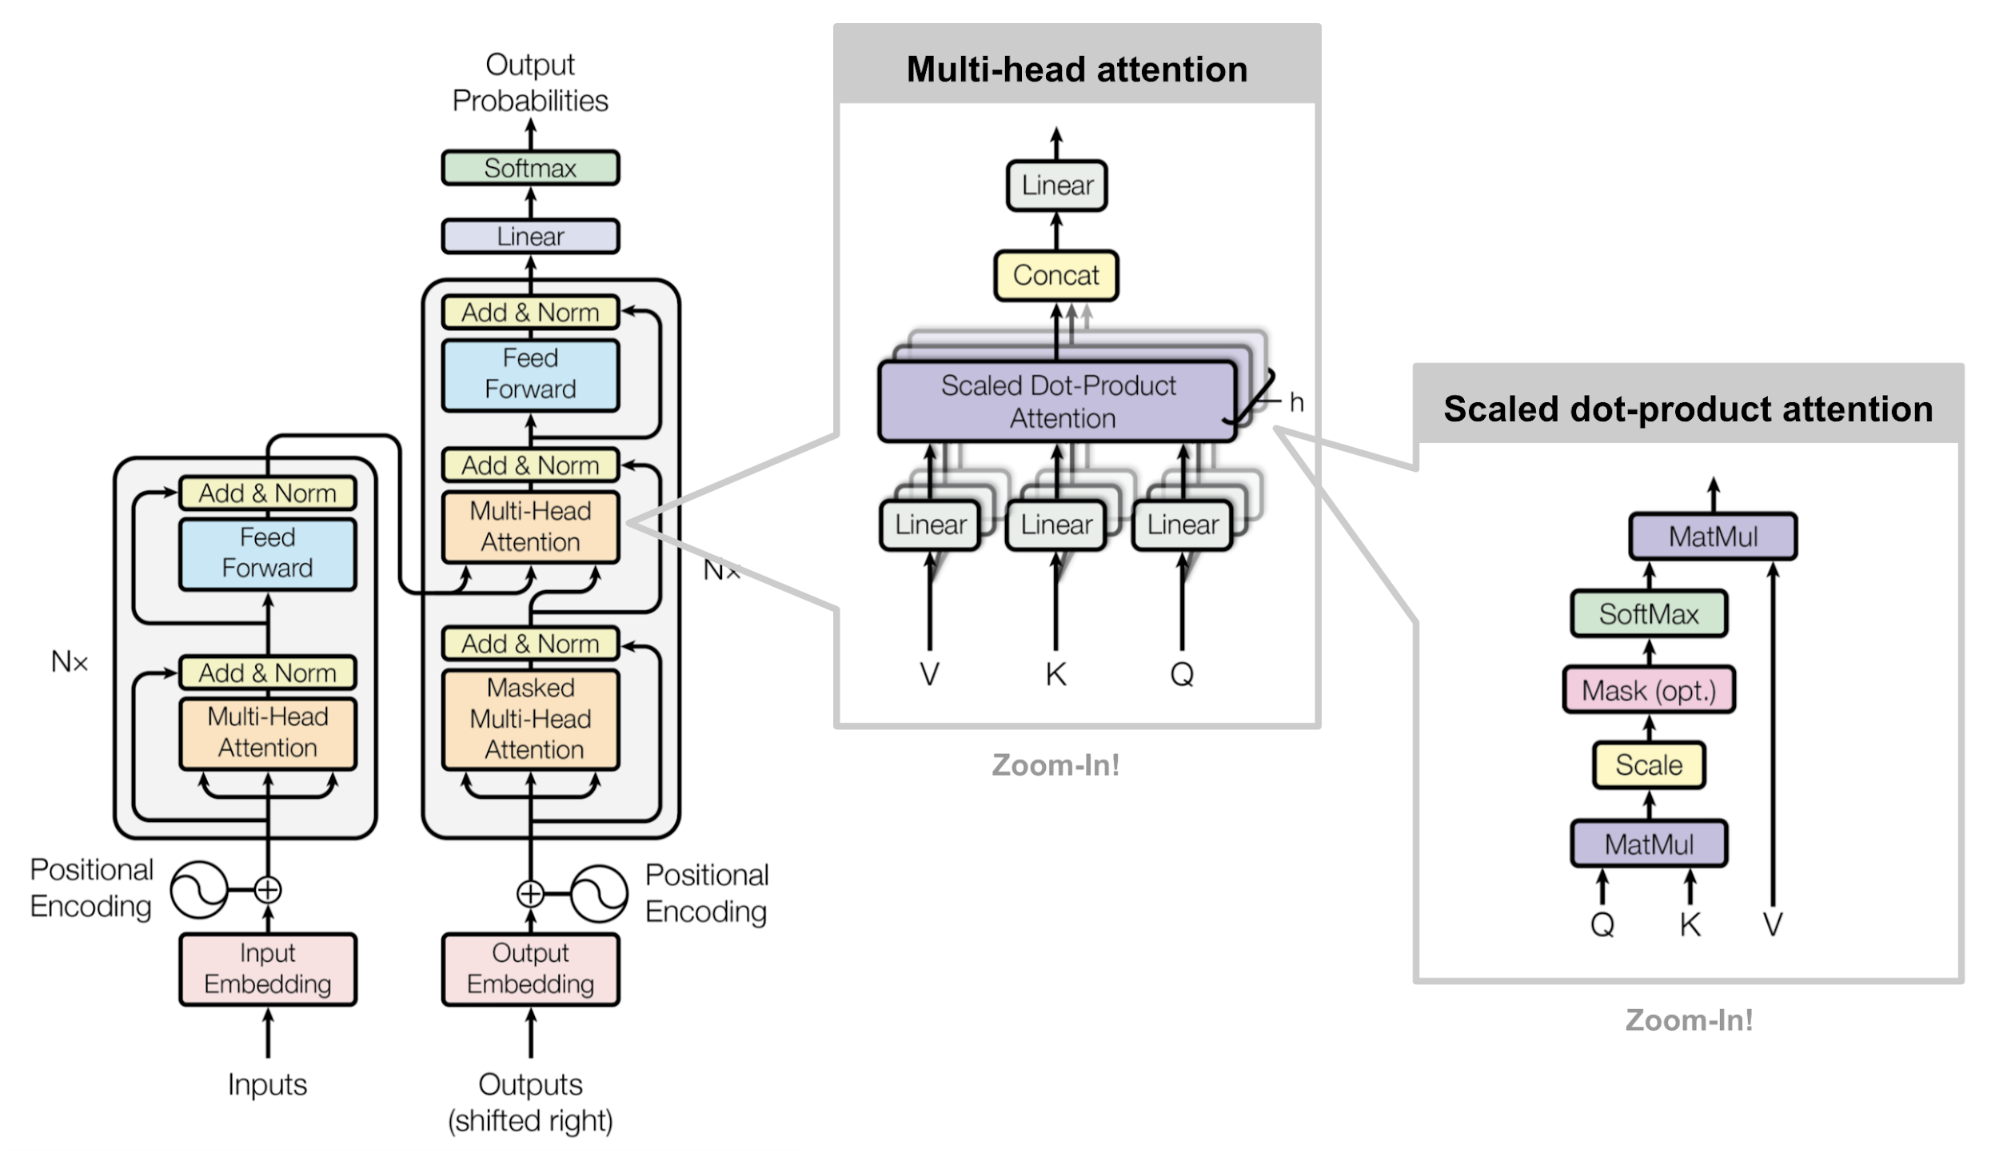
\includegraphics[width=0.95\textwidth]{imgs/transformer.png}
\vspace{-10pt}
\caption{\footnotesize Transformer model architecture. The gray boxes hold Encoder and Decoder layers, respectively, which are each repeated $N=6$ times. From \emph{Attention? Attention}, by Weng, 2018. \url{https://lilianweng.github.io/lil-log/2018/06/24/attention-attention.html}. Copyright 2018 by Weng.}
\vspace{-5pt}
\label{fig:transformer}
\end{figure}

The \textbf{Transformer model} introduced by Vaswani et al. (2017) for \nameref{nlptask:neuralmachinetranslationNMT} proves more parallelizable than general seq-to-seq models with attention. Rather than using \hyperref[sec:RNN]{ recurrent neural networks (RNNs)} combined with the \textbf{\hyperref[sec:AttentionMechanism]{attention mechanism}}, the Transformer sequence-to-sequence model uses only a \textbf{\hyperref[sec:SelfAttention]{self attention mechanism}} to attend to different word tokens in an input sentence and thus generate a sequence of \hyperref[sec:SolutionWithContextEmbs]{contextual embeddings}. It is illustrated in \cref{fig:transformer}.




\subsection{Self-Attention} \label{sec:SelfAttention}

\subsubsection{Motivation for Self-Attention}

{\large \textit{``The animal didn't cross the road because it was too tired."}}

%\begin{shadequote}{}
%\vspace{10pt}
%\large \textit{The animal didn't cross the road because it %was too tired.}
%\vspace{10pt}
%\end{shadequote}

What does ``it” in this sentence refer to? Is ``it" referring to the road or to the animal? This question may be simple to a human but not to a machine.  

This is the motivation for \textbf{self-attention}: when the Transformer processes the word ``it", self-attention allows it to associate ``it" with ``animal". As the Transformer processes each word, self-attention allows it to look at other positions in the input sentence for clues to create a better encoding for this word. In each layer, a part of the attention mechanism that focuses on ``the animal" was \emph{baked in} to a part of the representation of the word ``it" when encoding this in the model (Trevett, 2020). 


\subsubsection{Query, Key, Value} \label{sec:QKV}

Formally, ``an \textbf{\textit{attention function}} can be described as mapping a query and a set of key-value pairs to an output, where the \textbf{query, keys, values}, and output are all vectors. The output is computed as a weighted sum of the values, where the weight assigned to each value is computed by a compatibility function of the query with the corresponding key" (Vaswani et al., 2017). 

\begin{itemize}
    \item The Query matrix $Q$ contains row-wise information for which word to calculate self attention. 
    
     \item The Key matrix $K$ holds word vector representations on its rows, for \emph{each} word in the sentence.
     
    \item The Value matrix $V$ contains vector row-wise information for the rest of the words in the sentence. Multiplying the query vector with the key vector of a particular word, stored in $Q$ and $K$ computes a result that indicates how much \emph{value} vector $V$ to consider.
\end{itemize}

For the previous sentence, ``The animal didn't cross the road because it was too tired,"  $Q$ query refers to the word ``it"; $V$ contains vectors for words other than ``it", and $K$ contains vectors for each word, including ``it".  

The final embedding of the word or \textbf{output} is a weighted sum of \textbf{value} vectors and \hyperref[cnc:softmaxLayer]{softmax probabilities} of the dot product between query and key vectors: 
$$
Attention \Big(Q, K, V \Big) = softmax \Bigg(\frac {QK^T} {\sqrt{d_k}} \Bigg) V
$$
Each word has an associated \textbf{query, key, value} vector which are created by multiplying the words embeddings with parameter weight matrices $W^Q, W^K, W^V$ that are associated with the query, key, and value matrices, respectively. For the example sentence, let the input be the matrix $X = \{\overrightarrow{x_1}, \overrightarrow{x_2}, ..., \overrightarrow{x_n}\}$, where vector $\overrightarrow{x_i}$ corresponds to word $\overrightarrow{w_i}$, and there are $n$ words. Then the input word vectors are: 
% $
% \overrightarrow{x_1} = \text{"The"}, \!
% \overrightarrow{x_2} = \text{"animal"}, \!
% \overrightarrow{x_3} = \text{"didn't"}, \!
% \overrightarrow{x_4} = \text{"cross"}, \!
% \overrightarrow{x_5} = \text{"the"}, \!
% \overrightarrow{x_6} = \text{"road"}, \!
% \overrightarrow{x_7} = \text{because"}, \!
% \overrightarrow{x_8} = \text{"it"}, \!
% \overrightarrow{x_9} = \text{"was"}, \!
% \overrightarrow{x_{10}} = \text{"too"}, \!
% \overrightarrow{x_{11}} = \text{"tired"}, \!
% \overrightarrow{x_{12}} = "." 
% $

$$
\begin{array}{ll}
\overrightarrow{x_1} = \text{"The"} \\
\overrightarrow{x_2} = \text{"animal"} \\
\overrightarrow{x_3} = \text{"didn't"} \\
\overrightarrow{x_4} = \text{"cross"} \\
\overrightarrow{x_5} = \text{"the"} \\
\overrightarrow{x_6} = \text{"road"} \\
\overrightarrow{x_7} = \text{because"} \\
\overrightarrow{x_8} = \text{"it"} \\
\overrightarrow{x_9} = \text{"was"} \\
\overrightarrow{x_{10}} = \text{"too"} \\
\overrightarrow{x_{11}} = \text{"tired"} \\
\overrightarrow{x_{12}} = "." \\
\end{array}
$$
and the corresponding word embedding vectors are denoted $\Big\{ \overrightarrow{w_1}, \overrightarrow{w_2}, ..., \overrightarrow{w_n} \Big\}$ and the \textbf{query, key, value} matrices are denoted $Q = \Big\{\overrightarrow{q_1}, \overrightarrow{q_2}, ..., \overrightarrow{q_n} \Big\}$, $K = \Big\{\overrightarrow{k_1}, \overrightarrow{k_2}, ..., \overrightarrow{k_n} \Big\}$, $V = \Big\{\overrightarrow{v_1}, \overrightarrow{v_2}, ..., \overrightarrow{v_n} \Big\}$ respectively.


\subsubsection{Self-Attention: Vector Calculation}

Using notation from Vaswani et al. (2017) and Alammar (2018b), 

\begin{enumerate}
    \item \textbf{Create Query, Key, Value Vectors}: The first step is to create query, key, value vectors from each of the Encoder's input word embeddings $\overrightarrow{w_i}$ corresponding each word $\overrightarrow{x_i}$ by multiplying the embedding by appropriate rows in the three matrices obtained during training.  

    \item \textbf{Calculate a Score}: The scores determine how much \emph{focus to place on other parts of the input sentence} while encoding a word at a certain position.  The score is calculated by taking the dot product of the \textbf{query} vector with the \textbf{key} vector of the respective word being scored. Thus for word $\overrightarrow{w_i}$, the scores are: 
    $$
    \text{scores}_{\Large w_i} = \bigg\{
    \overrightarrow{q_i} \cdot \overrightarrow{k_1},
    \overrightarrow{q_i} \cdot \overrightarrow{k_2},
    ...,
    \overrightarrow{q_i} \cdot \overrightarrow{k_n} \bigg\}
    $$

    \item \textbf{Scale The Score}: The scores are scaled using $d_k$, which is the dimension of the key vector. From Vaswani et al. (2017), ``for large values of $d_k$, the dot products grow large in  magnitude, forcing the \hyperref[cnc:softmaxLayer]{softmax function} into regions where it has extremely small gradients. To counteract this effect, we scale the dot products by $\frac {1} {\sqrt{d_k}}$." Thus the scores for $\overrightarrow{w_i}$ are:
    $$
    \text{scores}_{\overrightarrow{w_i}} = \Bigg\{
    \frac {\overrightarrow{q_i} \cdot \overrightarrow{k_1}} {\sqrt{d_k}},
    \frac {\overrightarrow{q_i} \cdot \overrightarrow{k_2}} {\sqrt{d_k}},
    ...,
    \frac{\overrightarrow{q_i} \cdot \overrightarrow{k_n}} {\sqrt{d_k}} \Bigg\}
    $$
    
    \item \textbf{Apply Softmax}: The \hyperref[cnc:softmaxLayer]{softmax function} normalizes the scores into probabilities. 
    $$
    \text{scores}_{\overrightarrow{w_i}} = softmax \Bigg( \Bigg\{
    \frac {\overrightarrow{q_i} \cdot \overrightarrow{k_1}} {\sqrt{d_k}},
    \frac {\overrightarrow{q_i} \cdot \overrightarrow{k_2}} {\sqrt{d_k}},
    ...,
    \frac{\overrightarrow{q_i} \cdot \overrightarrow{k_n}} {\sqrt{d_k}} \Bigg\} \Bigg)
    $$

    \item \textbf{Compute the Weights}: The weighted values for word embedding $\overrightarrow{w_i}$ are calculated by multiplying each value vector in matrix $V$ by the \hyperref[cnc:softmaxLayer]{softmax} scores. Intuitively, this cements the values of words to focus on while drowning out irrelevant words. 
    $$
    \text{weights}_{\overrightarrow{w_i}} = \text{scores}_{\overrightarrow{w_i}} * (\overrightarrow{v_1}, ..., \overrightarrow{v_n})
    $$

    \item \textbf{Compute Output Vector}: The weight vector's cells are summed to produce the \textbf{output vector} of the self-attention layer for word embedding $\overrightarrow{w_i}$: 
    $$
    \overrightarrow{output_{w_i}} = softmax \Bigg(
    \frac {\overrightarrow{q_i} \cdot \overrightarrow{k_1}} {\sqrt{d_k}} \Bigg) \cdot \overrightarrow{v_1} +
    softmax \Bigg(\frac {\overrightarrow{q_i} \cdot \overrightarrow{k_1}} {\sqrt{d_k}} \Bigg) \cdot \overrightarrow{v_2} + ... +
    softmax \Bigg(\frac {\overrightarrow{q_i} \cdot \overrightarrow{k_1}} {\sqrt{d_k}} \Bigg) \cdot \overrightarrow{v_n}
    $$
\end{enumerate} 


\subsection{Self-Attention: Matrix Calculation}

Using notation from Vaswani et al. (2017) and Alammar (2018b), 

\begin{enumerate}
    \item \textbf{Calculate Query, Key, Value Matrices}: The word embeddings are packed into the rows of input matrix $X$ and this is multiplied by each of the trained parameter matrices $W^Q$, $W^K$, $W^V$ to produce the $Q$, $K$, $V$ matrices:
    $$
    \begin{array}{ll}
    Q = X \cdot W^Q \\
    K = X \cdot W^K \\
    V = X \cdot W^V 
    \end{array}
    $$
    
    \item \textbf{Calculate Self Attention}: Steps 2 through 6 of the vector calculation for self attention can be condensed into a single matrix step where $Q = \Big\{\overrightarrow{q_1}, \overrightarrow{q_2}, ..., \overrightarrow{q_n} \Big\}$, $K = \Big\{\overrightarrow{k_1}, \overrightarrow{k_2}, ..., \overrightarrow{k_n} \Big\}$, $V = \Big\{\overrightarrow{v_1}, \overrightarrow{v_2}, ..., \overrightarrow{v_n} \Big\}$: 
    $$
    Attention(Q, K, V) = softmax \Bigg(\frac {QK^T} {\sqrt{d_k}} \Bigg) \cdot V
    $$
\end{enumerate}


\subsection{Multi-Head Attention} \label{sec:MultiHeadAttention}

\subsubsection{Motivation for Multi-Head Attention}


A \textbf{multi-head attention mechanism} comprises of several self-attention heads, enabling the Transformer to ``jointly attend to information from different representation subspaces at different positions." A single attention head cannot do this because of averaging (Vaswani et al., 2017).  

While a single attention function has $d_{model}$-dimensional keys, values and queries, a multi-head attention function ``linearly projects the queries, keys and values $H$ (number of attention heads) times with different, learned linear projections to $d_k$, $d_k$, and $d_v$ dimensions, respectively." Instead of calculating attention once, multi-head attention does self attention many times in parallel on the projected dimensions, concatenates the independent attention outputs, and once again projects the result into the expected dimension to give a final value (Vaswani et al., 2017; Weng, 2018).  

For the example sentence, adding more attention heads enables the Transformer to focus on different words while encoding the meaning of word ``it." As ``it" is encoded, one attention head may focus most on ``the animal" while another focuses on ``tired", so the model's representation of ``it" incorporates some representation of all the words in the sentence (Trevett, 2020). 

\subsubsection{Multi-Head Attention: Matrix Calculation}

Using notation from Vaswani et al. (2017) and Alammar (2018b): 

\begin{enumerate}
    \item \textbf{Create $Q$, $K$, $V$ matrices}: With multi-headed attention there are now separate $Q$, $K$, $V$ weight matrices for each attention head $h$, in $1 \leq h \leq H$. The rows of input matrix $X$ correspond to a word in the input sentence, as before. For each attention head, $X$ is multiplied by trained parameter matrices to produce the separate query, key, value matrices: 
    $$
    Q_h = X \cdot W_h^Q \\
    K_h = X \cdot W_h^K \\
    V_h = X \cdot W_h^V 
    $$
    where $H =$ number of attention heads, and the dimensions of the parameter matrices are $\large W_h^Q \in \mathbb{R}^{\Large d_{model} \times d_k}$, $\large W_h^K \in \mathbb{R}^{\Large d_{model} \times d_k}$, $\large W_h^V \in \mathbb{R}^{\Large d_{model} \times d_v}$. 
    
    \item \textbf{Apply Softmax To Get Output Matrix}: Steps two through six in the vector calculation of self-attention can be condensed in a single matrix step to find the final output matrix $Z_h$ for the $h$-th attention head for any self-attention layer:
    $$
    Z_h := softmax \Bigg(\frac {Q_h K_h^T} {\sqrt{d_k}} \Bigg) \cdot V_h
    $$
    
    \item \textbf{Concatenate Output Matrices}: Now there are $H$ different output matrices $Z$ for each attention head. But the feed-forward layer is only expecting a single matrix instead of $H$. Thus, this step concatenates the $H$ matrices and multiplies the result by an additional weights matrix $W^O$ to return to expected dimensions. 
    $$
    MultiHeadAttention(Q, K, V) = Concat(head_1, ..., head_H) \cdot W^O
    $$
      where $head_i = Attention(Q \cdot W_h^Q, K \cdot W_h^K, V \cdot W_h^V)$, where the attention function is simply $Attention(Q, K, V) = softmax \Bigg( \frac {\Large QK^T} {\Large \sqrt{d_k}} \Bigg) \cdot V$. The parameter matrices have the following dimensions:  $W^O \in \mathbb{R}^{\Large H \cdot d_v \times d_{model}}$, $\large W_h^Q \in \mathbb{R}^{\Large d_{model} \times d_k}$, $\large W_h^K \in \mathbb{R}^{\Large d_{model} \times d_k}$, $\large W_h^V \in \mathbb{R}^{\Large d_{model} \times d_v}$
    
    
\end{enumerate}



\subsection{Positional Encodings} \label{sec:PosEncodings}

\subsubsection{Motivation for Positional Encodings}

Since the Transformer contains no recurrence mechanism it does not yet account for \emph{order in the sequence sentence}. Vaswani et al. (2017) found that injecting information about relative or absolute position of tokens in the sequence in the form of \textbf{positional encodings} helps resolve this issue. 
Otherwise, the sentences ``I like dogs more than cats" and ``I like cats more than dogs" would encode the same meaning (Raviraja, 2019). 

\subsubsection{Describing Positional Encodings}

A \textbf{positional encoding} follows a specific, learned pattern to identify word position or the distance between words in the sequence (Alammar, 2018b). The Transformer adds the positional encoding vector to each input embedding in both Encoder and Decoder stacks.   

According to Vaswani et al. (2017), positional encodings use sinusoidal waves to allow the Transformer to more easily attend to relative positions since for any fixed offset $k$, the positional encoding $\textit{PosEnc}_{\textit{pos} + k}$ can be represented as a linear function of $\textit{PosEnc}_{\textit{pos}}$.
$$
\begin{array}{ll}
\textit{PosEnc}_{\Large (\textit{pos}, 2i)} = \text{sin} \Bigg(\frac {\textit{pos}} {10000^{\Large \frac {2i} {d_{\textit{model}}} } }  \Bigg) \\
\textit{PosEnc}_{\Large (\textit{pos}, 2i + 1)} = \text{cos} \Bigg(\frac {\textit{pos}} {10000^{\Large \frac {2i} {d_{\textit{model}}} } }  \Bigg)
\end{array}
$$
where $\textit{pos} = $ a position, $i = $ a dimension.


\subsection{Position-wise Feed Forward Layer} \label{sec:PositionwiseFFNLayers}

A \textbf{positionwise feed-forward layer} is a kind of \hyperref[sec:NeuralNetRepr]{feed-forward neural network (FNN)} that is also ``position-wise" because the FFN is applied to each position separately and identically. The FFN contains two linear transformations with a $\textit{ReLU}$ or $\textit{max}$ activation function in between them:
$$
\textit{FFN}(x) = \textit{ReLU}(0, x W_1 + b_1) W_2 + b_2
$$

\subsection{Residual Connection} \label{sec:ResidualConnections}

A \textbf{residual connection} is a sub-layer in both Encoder and Decoder stacks which adds inputs to outputs of a sub-layer. This allows gradients during optimization to flow through a network directly rather than being transformed by nonlinear activations (Raviraja, 2019): 
$$
\textit{LayerNorm}(x + \textit{Sublayer}(x))
$$
where $\textit{Sublayer}(x)$ is a general function representing the sub-layer's operation. Each sub-layer in the stack, such as \hyperref[sec:SelfAttention]{self-attention} and \hyperref[sec:PositionwiseFFNLayers]{positionwise feed forward layer}s, are surrounded by residual connection layers followed by layer normalization. 




\subsection{Masked Multi-Head Attention} \label{sec:MaskedMultiHeadAttention}

The \textbf{masked self attention} is an \hyperref[sec:AttentionMechanism]{attention mechanism} that forms a sub-layer in the Decoder stack. It uses \textbf{masking} to prevent positions from attending to subsequent positions. Rather, while decoding a word embedding $\overrightarrow{w_i}$, the Decoder is not aware of words  $\overrightarrow{w_{>i}}$ past position $i$. It can only use words $\overrightarrow{w_{\leq i}}$. This masking is done to render invisible the words $\overrightarrow{w_{>i}}$ so that no superfluous predictions can be made (Ta-Chun, 2018). 

\subsection{Encoder-Decoder Attention} \label{sec:EncoderDecoderAttention}

This \hyperref[sec:AttentionMechanism]{attention layer} differs from attention layers found in either Encoder or Decoder. It is like \hyperref[sec:MultiHeadAttention]{multi-head self attention} but the difference is that the \textbf{encoder-decoder attention layer} creates the query matrix $Q$ from the layer below it (a Decoder self attention layer) and uses the key $K$ and value $V$ matrices from the Encoder stack's output (Alammar, 2018b). 



\subsection{Encoder} \label{sec:TransformerEncoder}

The Encoder is a \textbf{\hyperref[sec:BidirectionalLM]{bidirectional} \hyperref[sec:RNN]{recurrent network (RNN)}} consisting of a \hyperref[sec:ForwardLM]{forward} RNN and \hyperref[sec:BackwardLM]{backward} \hyperref[sec:RNN]{RNN}. The \hyperref[sec:ForwardLM]{forward} \hyperref[sec:RNN]{RNN} reads the input sequence $\overrightarrow{x} = \Big\{ x_1,...,x_{T_x} \Big\}$ from left to right to produce a sequence of forward hidden states $\Big\{ \overrightarrow{h_1},..., \overrightarrow{h_{T_x}} \Big\}$. The \hyperref[sec:BackwardLM]{backward} RNN reads the sequence in reverse order, so taking $x_{T_x}$ to $x_1$ and returns a sequence of backward hidden states $\Big\{ \overleftarrow{h_1},..., \overleftarrow{h_{T_x}} \Big\}$. Then, for each word $x_t$ an annotation is obtained by concatenating the corresponding forward hidden state vector $\overrightarrow{h}_t$ with the backward one $\overleftarrow{h}_t$, such that $h_t = \Big \{ \overrightarrow{h}_t^T \; ; \; \overleftarrow{h}_t^T \Big\}^T , \: t=1,...,T_x$. (Note: arrows here denote the direction of the network rather than vector notation.) This allows the annotation vector $h_t$ for word $x_t$ to contain contextual information by using previous and latter words (Bahdanau et al., 2016). These annotations are later used in the decoder to compute the context vector.  

The Encoder is composed of $N$ identical \textbf{Encoder layers}, which together are named the \textbf{Encoder stack}. A single \textbf{Encoder layer}  is composed of two sub-layers: 
\begin{enumerate}
    \item \textbf{ \nameref{sec:MultiHeadAttention} (layer)}
    
    \item \textbf{ \nameref{sec:PositionwiseFFNLayers} (layer)}
\end{enumerate}

A \hyperref[sec:ResidualConnections]{residual connection layer} surrounds each of these sub-layers, and is followed by \textbf{layer normalization} (Trevett, 2020).  




\begin{figure}[h]
\vspace{-10pt}
\centering
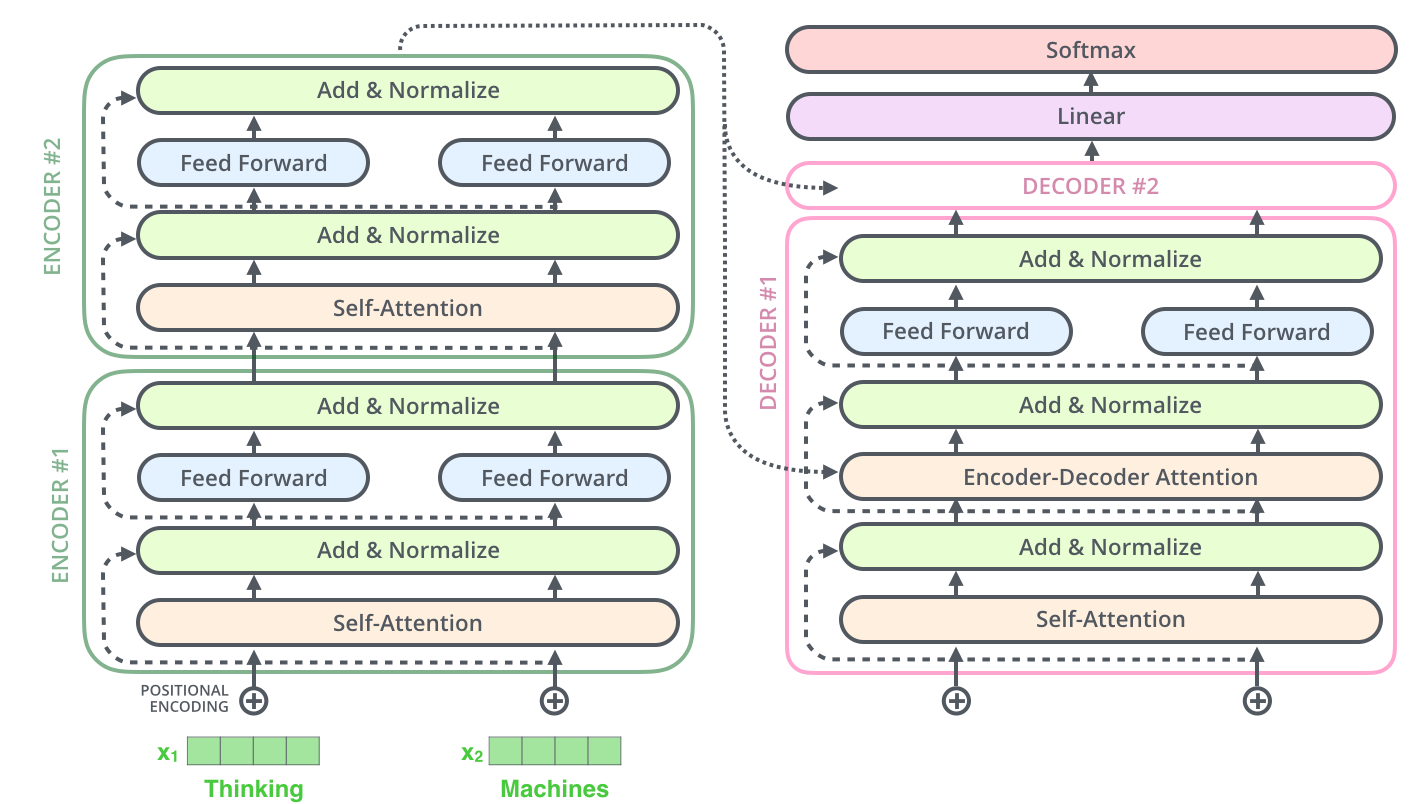
\includegraphics[width=0.8\textwidth]{imgs/encoderDecoderLayersDetailed.png}
\vspace{-10pt}
\caption{\footnotesize The layers inside Encoder and Decoder. From \emph{The Illustrated Transformer}, by Alammar, 2018. \url{https://jalammar.github.io/illustrated-transformer/}. Copyright 2018 by Alammar.}
\vspace{-5pt}
\label{fig:encDecLayersDetailed}
\end{figure}




\subsection{Decoder} \label{sec:TransformerDecoder}


The Decoder \hyperref[sec:NeuralLM]{neural network} generates hidden states $s_t = \text{Decoder}\Big( s_{t-1}, y_{t-1}, c_t \Big)$ for time steps $t = 1,..., m$ where the context vector $c_t = \sum_{i=1}^n \alpha_{ti} \cdot h_i$ is a sum of the hidden states of the input sentence, weighted by alignment scores, as for the \hyperref[sec:Seq2Seq]{Seq-to-Seq} model (Weng, 2018). 

Similarly to the Encoder, the Decoder contains a stack of $N$ Decoder layers, each of which consist of several sub-layers:
\begin{enumerate}
    \item \textbf{ \nameref{sec:MaskedMultiHeadAttention} (layer)}
    \item \textbf{ \nameref{sec:EncoderDecoderAttention} (layer)} 
    \item \textbf{ \nameref{sec:PositionwiseFFNLayers} (layer) }. 
\end{enumerate}

Like in the Encoder, in between each of these layers is a \hyperref[sec:ResidualConnections]{residual connection} followed by layer normalization. The Encoder and Decoder stack are shown in \cref{fig:encDecLayersDetailed}. 




\subsection{Final Linear and Softmax Layer} \label{sec:TransformerFinalLayer}


The Decoder stack outputs a vector of floats which is converted to a word using a Linear layer, followed by a Softmax layer in the Transformer neural network (Alammar, 2018b). 
\begin{itemize}
    \item \textbf{Linear Layer} is a simple, \hyperref[sec:NeuralLM]{fully-connected neural network} that projects the Decoder's output vector in a larger-dimension ``logits vector" in which each cell holds a score corresponding to each unique vocabulary word. 
    
    \item \textbf{Softmax Layer} then converts the Linear Layer's scores into probabilities via the \hyperref[cnc:softmaxLayer]{softmax function}. 
\end{itemize}

To find the predicted word, the cell with highest probability is chosen, and corresponding word is called the predicted word, and is output for a particular time step.




\subsection{Transformer Workflow} \label{sec:TransformerWorkflow}

Alammar (2018b) describes the procedure governing the Transformer's moving parts as follows: 

\begin{enumerate}
    \item The \nameref{sec:TransformerEncoder} processes the input sentence in the given language, adding the \hyperref[sec:PosEncodings]{positional encoding} to input embeddings.
    
    \item The output of the top \nameref{sec:TransformerEncoder} layer is then transformed into a set of \hyperref[sec:AttentionMechanism]{attention} vectors $K$ and $V$.
    
    \item The \nameref{sec:TransformerDecoder} uses $K$ and $V$ in its \hyperref[sec:EncoderDecoderAttention]{encoder-decoder attention layer} to help the \nameref{sec:TransformerDecoder} focus on appropriate places in the input sequence. Subsequent outputs are fed to the bottom \nameref{sec:TransformerDecoder}, allowing \nameref{sec:TransformerDecoder}s to accumulate results. Also, the \nameref{sec:TransformerDecoder} includes \hyperref[sec:PosEncodings]{positional encoding}s to its inputs. 
    
    \item The previous steps are repeated until a special symbol is reached, indicated the \nameref{sec:TransformerDecoder} has finished generating output.
    
    \item The \nameref{sec:TransformerDecoder}'s numeric output vector is passed through the \hyperref[sec:TransformerFinalLayer]{final linear and softmax layer} to find a predicted, translated word in the target language. 
    
\end{enumerate}

% done
\section{ELMo} \label{sec:ELMo}


\subsection{Combing Back To Polysemy} \label{sec:PolysemyAgainInElmo} 

As explained in \nameref{sec:ProblemWithStaticEmbs}, the term \textbf{\hyperref[sec:Polysemy]{polysemy}} is the correspondence of one word to distinct meanings, and traditional embeddings fail to capture these senses, thus performing poorly on language modeling \hyperref[app:Appendix_NLPTasks]{NLP tasks}. However, \hyperref[sec:SolutionWithContextEmbs]{contextual embeddings (CWE)} prove superior since they create one vector representation for each word type in the vocabulary and also create distinct word vectors per token given a context (Wiedemann et al., 2019).   

For example, if instead models used only word and character embedding, the homonyms ``book" (text) and ``book" (reservation) would be assigned the \emph{same vector representation even though these are different words}. This vector representation may of course be created using context, as per the \nameref{sec:Word2Vec} or \nameref{sec:Glove}, but these meanings are still \emph{collapsed into a single representation}.


\subsection{Motivation for ELMo} 


In contrast to traditional word embeddings, \textbf{deep contextualized word embeddings} from Peters et al. (2018) capture word semantics to account for the context-dependent and polysemous nature of words.  

These word vectors are ``learned functions of the internal states of a \hyperref[sec:BidirectionalLM]{bidirectional language model (biLM)}" that is pretrained on a large corpus. Due to this, the resulting word embeddings are coined \textbf{ELMo (Embeddings from Language Models)}.  

\textbf{ELMo representations} are \emph{deep} since they are derived from all internal layers of the \hyperref[sec:BidirectionalLM]{biLM}. ELMo learns a ``linear combination of vectors stacked above each input word for each end task," improving performance of models that use only the top \hyperref[sec:LSTM]{LSTM} layer.  

Higher-level LSTM layers capture contextual meaning, useful for supervised \nameref{nlptask:wordsensedisambiguatioNWSD}, and lower layers capture syntax information, useful for \nameref{nlptask:postagging}. Coupled with the fact that mixing these signals allows the learned embeddings to select the types of semi-supervision most needed for each end task, ELMo embeddings are richer than traditional word vectors (Peters et al., 2018). 


\subsection{Describing ELMo} 

``ELMo is a task-specific combination of the intermediate layer representations in the \hyperref[sec:BidirectionalLM]{biLM}" (Peters et al., 2018). Formally, for each word token $t_k$, an $L$-layer \hyperref[sec:BidirectionalLM]{biLM} creates $2L + 1$ representations: 

$$
\begin{array}{ll}
R_k 
&= \Big \{ \mathbf{x}_k^{LM}, \; \overrightarrow{\mathbf{h}}_{kj}^{LM}, \; \overleftarrow{\mathbf{h}}_{kj}^{LM} \; | \; j = 1,...,L \Big \} \\
&= \Big \{ \mathbf{h}_{kj}^{LM} \; | \; j = 1,...,L \Big \}
\end{array}
$$
where $\mathbf{h}_{k0}^{LM}$ is the token layer and the hidden state vector $\mathbf{h}_{kj}^{LM} = \Big \{ \overrightarrow{\mathbf{h}}_{kj}^{LM}, \; \overleftarrow{\mathbf{h}}_{kj}^{LM}  \}$, a concatenation of backward and forward hidden states, for each \hyperref[sec:BidirectionalLM]{bidirectional} \hyperref[sec:LSTM]{LSTM} layer. ELMo collapses all layers in the above vector into a single ``ELMo" embedding ready for a specific task, by weighting the \hyperref[sec:BidirectionalLM]{biLM} layers in a task-specific way (Peters et al., 2018): 
$$
\textbf{ELMo}_k^{task} = E \Big( R_k; \theta^{task} \Big) = \gamma^{task} \; \sum_{j=0}^L s_j^{task} \; \mathbf{h}_{kj}^{LM}
$$
where the vector $\mathbf{s}^{task} = \Big\{ s_j^{task} \Big\}$ of softmax-normalized weights and task-dependent scalar parameter $\gamma^{task}$ allow the model for the specific $task$ to scale the entire $\textbf{ELMo}_k^{task}$ vector. The index $k$ corresponds to a $k$-th word, and index $j$ corresponds to the $j$-th layer out of $L$ layers. Here, $h_{kj}^{LM}$ is the output of the $j$-th \hyperref[sec:LSTM]{LSTM} for word $k$, and $s_j$ is the weight of $h_{kj}^{LM}$ used to compute the representation for word $k$.   

The \hyperref[sec:BidirectionalLM]{biLM} in ELMo is task-agnostic, and ELMo combines the task-independent representations. Although the hidden states are fixed, this ELMo formulation is flexible enough to be combined in downstream models for various tasks (Kurita, 2018b). ELMo can be applied to specific tasks by concatenating the ELMo word embeddings with \hyperref[sec:StaticVsContextualEmb]{context-free word embeddings}, such as those from \nameref{sec:Glove}, Peters et al. (2018) say the concatenated input vector $\Big\{ \mathbf{x}_k \; ; \; \textbf{ELMo}_k^{task} \Big\}$ can be fed into a task-specific \hyperref[sec:RNN]{RNN} for processing. 

\subsection{ELMo Experimental Results} \label{sec:ResultsELMo}

\begin{itemize}
    \item  \textbf{\nameref{nlptask:questionansweringQA}: } Peters et al. (2018) added ELMo embeddings to a baseline \hyperref[sec:BidirectionalLM]{biLM} model with \hyperref[sec:AttentionMechanism]{attention} from Seo et al. (2017) and found this improved the test set $F_1$ score of the \hyperref[sec:BidirectionalLM]{biLM} model from $81.1 \%$ to $85.8 \%$, a state-of-the-art result. 

    \item \textbf{\nameref{nlptask:semanticrolelabelingSRL}: } When adding ELMo representations to an 8-layer deep biLSTM that interwove forward and backward directions, the single test set $F_1$ score increased by $3.2 \%$, which is a $1.2 \%$ improvement over the previous best model. 
    
    \item \textbf{\nameref{nlptask:coreferenceresolutionCR}: } Using Lee et al. (2017)'s model that uses \hyperref[sec:AttentionMechanism]{attention} to compute span vectors transformed by \hyperref[cnc:softmaxLayer]{softmax} ranking to find \hyperref[nlptask:coreferenceresolutionCR]{coreference} chains, adding ELMo embeddings improved the average $F_1$ score by $3.2 \%$, improving over the previous best model by nearly two percentage points. 
    
    \item \textbf{\nameref{nlptask:namedentityrecognitionNER}: } The baseline model had pretrained, character embeddings from a convolutional neural network (CNN), as well as two biLSTM layers and a conditional random field (CRF) loss function formulation (Lafferty et al., 2001). Adding ELMo embeddings $92.22 \%$ in $F_1$ score by letting the task model learn an average of all biLM layers, rather than only using the top layer. 
    
    \item \textbf{\nameref{nlptask:sentimentanalysisSA}: } A classification model using contextual embeddings from CoVe (McCann et al., 2018) was used as the baseline model, with CoVe embeddings replaced by ELMo embeddings. This resulted in a full percentage increase in absolute accuracy over state of the art. 
\end{itemize}


\subsubsection{ELMo's Key Feature} \label{sec:ELMoKeyFeature}

Because ELMo improves task performance over word embeddings, this must mean its \hyperref[sec:BidirectionalLM]{biLM}'s contextual representation outputs are encoding task-specific information that traditional word vectors do not otherwise capture. In other words, the \hyperref[sec:BidirectionalLM]{biLM} must be sifting meaning of words using their context.   


\begin{table}[ht!]
  \centering
  \begin{tabular}{ c }
    
    \begin{minipage}{.8\textwidth}
      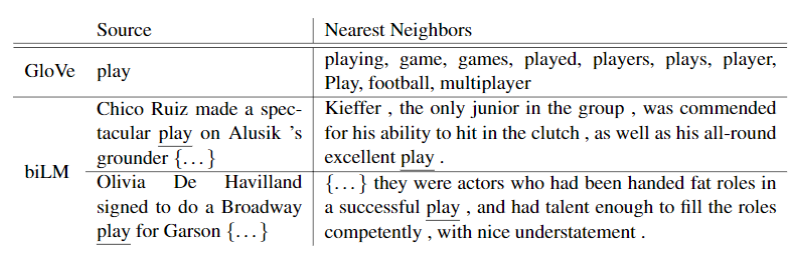
\includegraphics[width=\linewidth]{imgs/table_elmoPlay.png}
    \end{minipage}
    
  \end{tabular}
  \caption{\footnotesize Nearest neighbors to ``play” using GloVe and the context embeddings from a biLM. From \emph{Table 4 in Deep Contextualized Word Representations}, by Peters et al., 2018. \url{https://arxiv.org/pdf/1802.05365.pdf}. Copyright 2018 by Peters et al.}
  \label{tbl:elmoPlayExample}
\end{table}


The word ``play" is highly \hyperref[sec:PolysemyAgainInElmo]{polysemous} since it has many different meanings;  \cref{tbl:elmoPlayExample} displays words nearest to ``play" found using \nameref{sec:Glove} word embeddings and a \hyperref[sec:BidirectionalLM]{biLM} model. The \nameref{sec:Glove}'s neighbors include several different parts of speech, like verbs (``played", ``playing"), and nouns (``player", ``game") and only in the sport sense of the word. However, the bottom two rows show that the nearest neighbor sentences from the \hyperref[sec:BidirectionalLM]{biLM}'s contextual embedding of ``play" can disambiguate between \emph{both} the parts of speech \emph{and} word sense of ``play". The last row's input sentence contains the noun / acting sense of ``play" and this is matched in the nearest neighbor sentence, highlighting ELMo's ability to learn context using \nameref{nlptask:postagging} and \nameref{nlptask:wordsensedisambiguatioNWSD}. % done
\section{BERT} \label{sec:BERT}

\subsection{Problem with ELMo} \label{sec:ProblemWithELMo}

Simple word embedding models, unlike \hyperref[sec:LSTM]{LSTM}s, cannot capture combinations of words, negation and \hyperref[sec:Polysemy]{polysemy}. But \hyperref[sec:LanguageModels]{language models} have been effective at \emph{sentence-level} nlp tasks like natural language inference and paraphrasing, which predict sentence relationships, and also \emph{token-level} tasks like \nameref{nlptask:namedentityrecognitionNER} and \nameref{nlptask:questionansweringQA}, where a fine-grained approach is needed (Devlin et al., 2019).   

Previous methods like \textbf{ULMFiT} and \nameref{sec:ELMo} use a \hyperref[sec:BidirectionalLM]{bidirectional language model (biLM)} to account for left and right context. But the problem is that neither the \hyperref[sec:ForwardLM]{forward} \hyperref[sec:LSTM]{LSTM} nor the \hyperref[sec:BackwardLM]{backward} \hyperref[sec:LSTM]{LSTM} account for past and future tokens \textbf{\textit{at the same time.}} This deficiency does not let the model perform as well as it should since information from the entire sentence is not being used \textbf{\textit{simultaneously}}, regardless of position. 


\begin{figure}[h]
\vspace{-5pt}
\centering
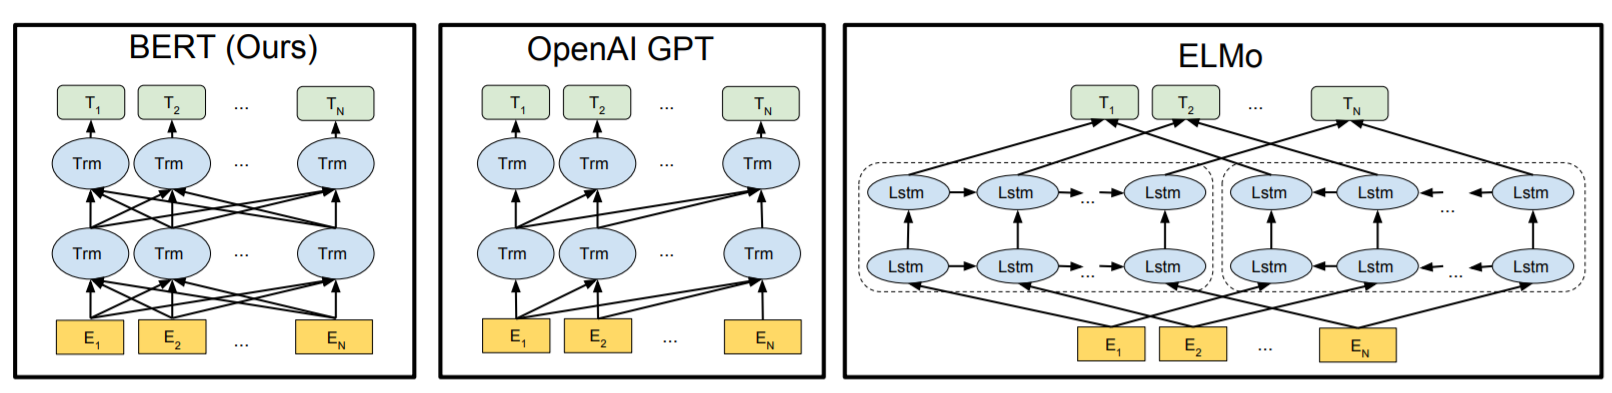
\includegraphics[width=0.9\textwidth]{imgs/bert_vs_elmo_vs_gpt.png}
\vspace{-5pt}
\caption{\footnotesize Comparing pre-training models: BERT uses a \hyperref[sec:BidirectionalLM]{bidirectional} \nameref{sec:Transformer}. OpenAI GPT uses a \hyperref[sec:ForwardLM]{forward} \nameref{sec:Transformer}. \nameref{sec:ELMo} combines independently-trained \hyperref[sec:ForwardLM]{forward} and \hyperref[sec:BackwardLM]{backward} \hyperref[sec:LSTM]{LSTM}s. Among the three, only BERT embeddings are jointly conditioned on forward and backward context in all layers. Alongside architectural differences, BERT and OpenAI GPT are fine-tuning approaches, while ELMo is a feature-based approach (Devlin et al., 2019). \textit{NOTE: $E_n =$ the $n$-th token in the input sequence, and $T_n =$ the corresponding output embedding}. From \emph{BERT: Pre-training of Deep Bidirectional Transformers for Language Understanding}, by Devlin et al., 2019. \url{https://arxiv.org/pdf/1810.04805.pdf}. Copyright 2019 by Devlin et al.}
\vspace{-5pt}
\label{fig:NAME}
\end{figure}





\subsection{Motivation for BERT} \label{sec:MotivationForBERT}

Instead of using \nameref{sec:ELMo}'s ``shallow" combination of ``independently-trained" \hyperref[sec:BidirectionalLM]{biLM}s, ``BERT is designed to pre-train deep bidirectional representations from unlabeled text by jointly conditioning on both left and right context in all layers" (Devlin et al., 2019).   


Another motivation for BERT stems from previous limitations. The \textbf{OpenAI GPT} model uses a left-to-right construction, where each token only attends to past tokens in the \hyperref[sec:SelfAttention]{self attention} layers of the \nameref{sec:Transformer}. This approach performs poorly on \emph{sentence-level} and \emph{token-level} tasks, like \nameref{nlptask:questionansweringQA}, where \textbf{bidirectional context} is required.  

\textbf{BERT (Bidirectional Encoder Representations from Transformers)} has progressed over past models since, in conjunction with its \hyperref[sec:BidirectionalLM]{biLM}, \hyperref[sec:SelfAttention]{self attention}, and \nameref{sec:Transformer} (more powerful than \hyperref[sec:LSTM]{LSTM}s), BERT uses a \hyperref[sec:maskedlanguagemodelMLM]{masked language model (MLM)} to avoid unidirectionality, resulting in vast performance gains over previous models (Wiedemann et al., 2019). 




\subsection{Describing BERT} \label{sec:DescribingBERT}

\subsubsection{Input Embedding in BERT} \label{sec:BERTInputEmbedding}

The input embedding in BERT is created by summing three kinds of other embeddings: 

\begin{enumerate}
    \item \textbf{\textit{WordPiece} token embeddings: }The \emph{WordPiece} \nameref{nlptask:tokenization} strategy, instead of tokenizing by the natural separations between English words, subdivides words into smaller, basic units. For example, the WordPiece \nameref{nlptask:tokenization} of ``playing" might be ``play" + ``**ing". This allows BERT to handle rare, unknown words (Weng, 2019) and reduce vocabulary size while increasing amount of data available per word. Consider: if ``play" and ``**ing" and ``**ed" are present in the vocabulary but ``playing" and ``played" are not, then these can be recognized by their sub-units. 
    
    \item \textbf{Segment embeddings: }are  arbitrary spans of contiguous text, rather than discrete sentences. The term ``sequence" for BERT refers to the input tokens, which can be parts of sentences or several sentences packed together. Contrary to BERT,  \nameref{sec:TransformerXL}'s \textbf{segment embeddings} respect sentence boundaries. 
    
    \item \textbf{\hyperref[sec:PosEncodings]{Positional embeddings}: } to account for word ordering. 
\end{enumerate}


\subsubsection{BERT's Framework}
 
There are two steps in BERT's framework: \textbf{pre-training}, in which BERT is trained on \emph{unlabeled data} over different tasks, and \textbf{fine-tuning}, in which BERT is initialized with the pre-training parameters to train over \emph{labeled data} for specific \hyperref[app:Appendix_NLPTasks]{nlp tasks}. Pre-training BERT using the \nameref{sec:maskedlanguagemodelMLM} task and \nameref{sec:nextsentencepredictionNSP} task allows BERT to learn \textbf{bidirectional context} and \emph{sentence-level} information, rather than just predict subsequent tokens given some context, as was the norm for simple \hyperref[sec:LanguageModels]{language models}.


\subsubsection{Masked Language Model (MLM)} \label{sec:maskedlanguagemodelMLM}

It is a well-known problem that bidirectional conditioning causes lower layers to leak information about tokens, so each word can implicitly ``see itself" letting the model trivially guess the target word in a multi-layered context (Devlin et al., 2019).  

BERT's solution is to use a \textbf{masked language model (MLM)}, which randomly masks some of the input tokens with the aim of predicting the original vocabulary id of the masked word using only its context. This fuses left and right context to get \emph{deep} bidirectional context, unlike \nameref{sec:ELMo}'s shallow left-to-right language model (Devlin et al., 2019).  

An issue with masking is that the model only predicts the \texttt{[MASK]} token when it is present in the input, while the intention was for the model to predict the correct tokens regardless of which tokens were present in input (Kurita, 2019a). This hampers performance since BERT would learn a contextual meaning of the mask token, causing it to learn slower since only $15 \%$ of tokens are masked. To resolve this, BERT varies its masking strategy: (1) replace the word to be masked with \texttt{[MASK]} only with $80\%$ probability; (2) replace the word to be masked with a random word $10 \%$ of the time; and (3) keep the masked word $10 \%$ of the time. For example, if the sentence was ``The cow jumped over the moon," and if the token to be masked was ``moon", then $80 \%$ of the time, the replacement would be ``The cow jumped over the \textbf{\texttt{[MASK]}}"; $10 \%$ of the time a random token would be used ``The cow jumped over the \textbf{seaweed}"; and the remaining times the sentence would remain the same. 



\subsubsection{Next Sentence Prediction (NSP)} \label{sec:nextsentencepredictionNSP}

Ordinary \hyperref[sec:LanguageModels]{language models} perform badly for tasks like \nameref{nlptask:questionansweringQA} and \nameref{nlptask:naturallanguageinferenceNLI} which require modeling sentence relationships, therefore BERT is pre-trained on a \textbf{next sentence prediction (NSP)} task for finding whether one sentence is the next sentence of the other. 

Training BERT using NSP is as follows: (1) sample sentence pairs \texttt{(A, B)} so that half the time \texttt{B} follows \texttt{A} (labeled as \texttt{IsNext}) and half the other time, \texttt{B} does not follow \texttt{A} (labeled as \texttt{NotNext}), then (2) BERT processes both sentences and uses a binary classifier to decide of \texttt{B} is the next sentence after \texttt{A} (Weng, 2019). 


\subsection{Experimental Results of BERT} \label{sec:BERTExperimentalResults}

% NOTE: the top width must be +0.5 more than below texwidth measure
\begin{program}
\begin{wrapfigure}{L}{0.75\textwidth}
    \begin{center}
    \vspace{-10pt}
    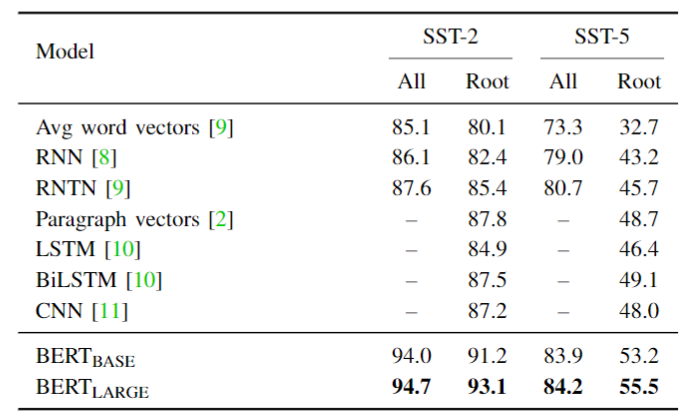
\includegraphics[width=0.6\textwidth]{imgs/table_bert_vsOtherModels.png}
    \end{center}
\vspace{-30pt}
\captionof{table}{\footnotesize Accuracy (\%) of several models on \nameref{nlptask:sentimentclassificationSC} SST dataset. BERT has highest accuracy scores. From \emph{Table B.II in Fine-Grained Sentiment Classification Using BERT}, by Munikar et al., 2019. \url{https://arxiv.org/pdf/1910.03474.pdf}. Copyright 2019 by Munikar et al.}
\label{tbl:bertExperimentResults}
\end{wrapfigure}


Using a simple accuracy measure, Munikar et al. (2019) found that a pre-trained BERT model fine-tuned for \nameref{nlptask:sentimentanalysisSA} task outperformed complex models such as \hyperref[sec:RNN]{RNN}s and CNNs. The \cref{tbl:bertExperimentResults} includes results on phrases and entire reviews. 


This proves \nameref{nlptask:transferlearning} is possible with BERT's deep contextual \hyperref[sec:BidirectionalLM]{bidirectional language model}.
\end{program}


\subsection{Probing BERT} \label{sec:ProbingBERT}

BERT has surpassed state-of-the-art performance in a wide range of \hyperref[app:Appendix_NLPTasks]{nlp tasks} but it is not known why. Clark et al. (2019) use an ``attention-based probing classifier" to study BERT's internal vector representations to understand what kinds of linguistic features BERT learns from its self-supervised training on unlabeled data. 



\subsubsection{BERT Learns Dependency Syntax} \label{sec:BERTLearnsSyntax}

Firstly, Clark et al. (2019) found that BERT's attention heads behave similarly, like focusing on positional offsets or attending broadly over an entire sentence. 

Secondly, while individual attention heads do not capture syntax dependency structure as a whole, it was found that certain attention heads are better at detecting various syntax dependency relations. For example, the heads detect ``direct objects of verbs, determiners of nouns, objects of prepositions, and objects of possessive pronouns with > $75 \%$ accuracy (Clark et al., 2019). 

\begin{figure}
\centering
\begin{minipage}{.4\textwidth}
  \centering
  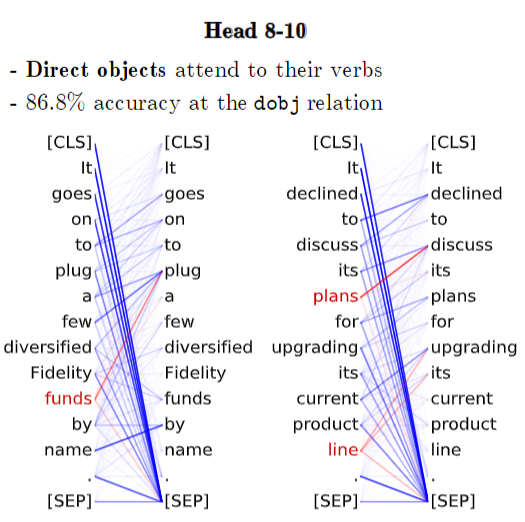
\includegraphics[width=\textwidth]{imgs/bert_headsDirectObject.png}
  \captionof{figure}{\footnotesize BERT attention heads capture syntax. In heads 8-10, direct objects are found to attend to their verbs. Line darkness indicates attention strength. Red indicates attention to/from red words, to highlight certain attentional behaviors. From \emph{What Does BERT Look At? An Analysis of BERT's Attention}, by Clark et al., 2019. \url{https://arxiv.org/abs/1906.04341}. Copyright 2019 by Clark et al.}
  \label{fig:bertHeadDirectObject}
\end{minipage} \hspace{2em}%
\begin{minipage}{.4\textwidth}
  \centering
  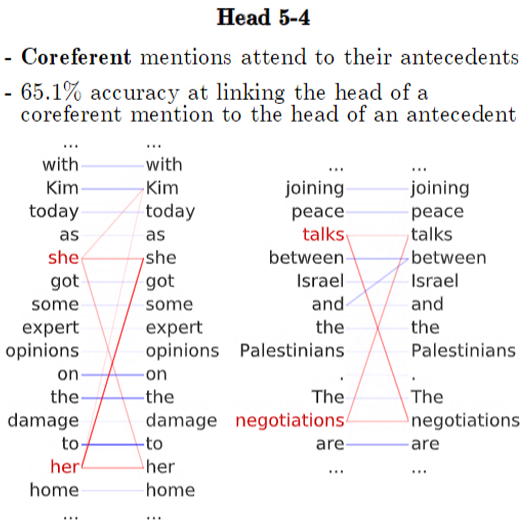
\includegraphics[width=\textwidth]{imgs/bert_headsCoref.png}
  \captionof{figure}{\footnotesize BERT attention heads capture syntax. In heads 5-4, BERT does some \nameref{nlptask:coreferenceresolutionCR} with high accuracy at linking the head of a coreferent mention to the head of an antecedent. From \emph{What Does BERT Look At? An Analysis of BERT's Attention}, by Clark et al., 2019. \url{https://arxiv.org/abs/1906.04341}. Copyright 2019 by Clark et al.}
  \label{fig:bertCoref}
\end{minipage}
\end{figure}


Attention heads 8-10 in \cref{fig:bertHeadDirectObject} learn how direct objects attend to their verbs, and achieves high accuracy at the direct object relation task. The fact that BERT learns this via self-supervision coupled with the heads' propensity for learning syntax may explain BERT's success. Attention heads 5-4 in \cref{fig:bertCoref} perform \nameref{nlptask:coreferenceresolutionCR}. This task is more challenging than syntax tasks since \hyperref[nlptask:coreferenceresolutionCR]{coreference} links span longer than syntax dependencies, and even state-of-the-art models struggle at this task.




\subsubsection{BERT's Limitation In Segment-Level Representation}

Instead of using separator tokens to gather segment-level information, BERT actually views separator tokens \texttt{[SEP]} as ``no-op" or stub operations for attention heads when the head is not needed for a current task. 

\begin{figure}[h]
\vspace{-5pt}
\centering
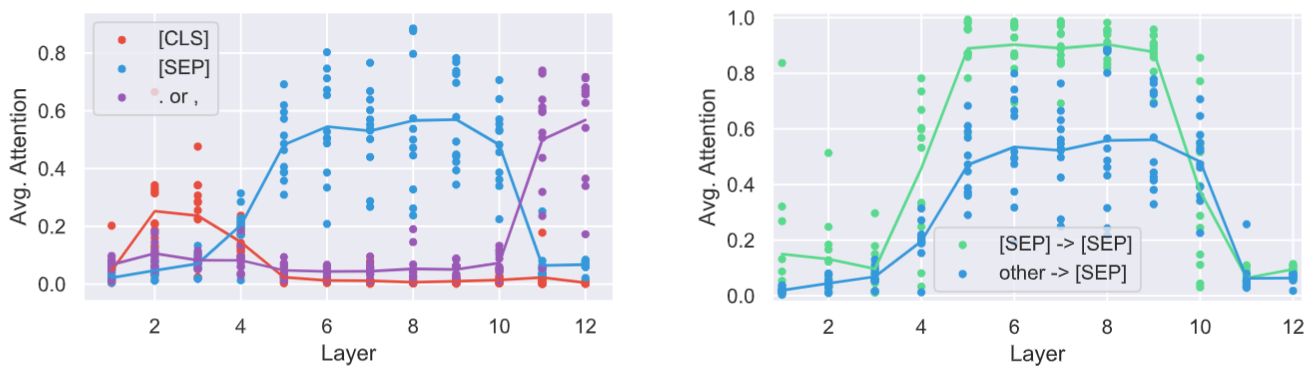
\includegraphics[width=0.95\textwidth]{imgs/bert_attentionheads_SEP.png}
\vspace{-5pt}
\caption{\footnotesize BERT's attention heads in layers 6-10 spend more than half the average attention to separator tokens; deep heads attend to punctuation, while middle heads attend to \texttt{[SEP]}, and early heads attend to \texttt{[CLS]}. From \emph{What Does BERT Look At? An Analysis of BERT's Attention}, by Clark et al., 2019. \url{https://arxiv.org/abs/1906.04341}. Copyright 2019 by Clark et al.}
\vspace{-5pt}
\label{fig:bertSEPAttention}
\end{figure}

Authors hypothesized as to why so many of BERT's attention heads focus on separator tokens, a feature visible in \cref{fig:bertSEPAttention}. But there are several investigations that prove this may not be the case: 
\begin{enumerate}
    \item If BERT were indeed trying to gather segment-level information, then attention heads processing \texttt{[SEP]} should attend broadly over the entire segment to create the segment representations. But \cref{fig:bertHeadDirectObject} shows that in heads 8-10 direct objects attend to their verbs, while all other words attend to the \texttt{[SEP]} token. 
    
    \item Gradient measures were used to study how much the attention to a token would change BERT's outputs. While attention to \texttt{[SEP]} increases from layer 5 onwards (visible in \cref{fig:bertSEPAttention}), the gradients for attention to \texttt{[SEP]} decrease substantially (visible in \cref{fig:bertGradient}). This means attending to \texttt{[SEP]} does not significantly change BERT's outputs. 
\end{enumerate}


\begin{figure}[h]
\vspace{-5pt}
\centering
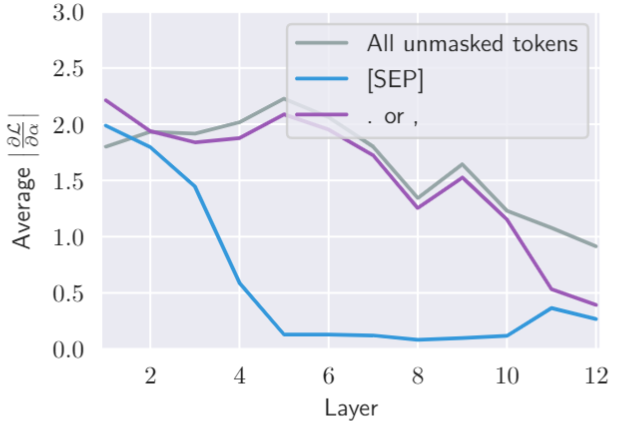
\includegraphics[width=0.45\textwidth]{imgs/bert_attentionheads_gradient.png}
\vspace{-5pt}
\caption{\footnotesize Gradient-based estimates for attention to separator and punctuation tokens. Authors ``compute the magnitude of the gradient of the loss from the \nameref{sec:maskedlanguagemodelMLM} task with respect to each attention weight." From \emph{What Does BERT Look At? An Analysis of BERT's Attention}, by Clark et al., 2019. \url{https://arxiv.org/abs/1906.04341}. Copyright 2019 by Clark et al.}
\vspace{-5pt}
\label{fig:bertGradient}
\end{figure}



The above two investigations suggest BERT's attention heads only attend to \texttt{[SEP]} when they have no other job, not to gather segment-level information. However, \nameref{sec:TransformerXL} by design improves over BERT in this regard. 









\subsubsection{BERT's Contribution To Polysemy} % PAPER: DOEs bert make any sense

Using a kNN classification, Wiedemann et al. (2019) compared the \hyperref[sec:SolutionWithContextEmbs]{contextual embeddings (CWE)s} of \nameref{sec:ELMo} and BERT on the \nameref{nlptask:wordsensedisambiguatioNWSD} task and found that BERT places \hyperref[sec:Polysemy]{polysemic} words into distinct regions according to their senses, while \nameref{sec:ELMo} cannot. Specifically, in \nameref{sec:ELMo} embeddings, major word senses are less strongly separated than in the BERT embedding space, where some senses are sharply clustered. 

In \cref{tbl:bertPolysemy} Wiedemann et al. (2019) also made inferences about the semantic features of BERT's embeddings by studying how BERT matched word senses from the test set to a given \hyperref[sec:Polysemy]{polysemic} word from a training set.



\begin{table}[ht!]
  \centering
  \caption{\footnotesize Example predictions by BERT based on nearest neighbor sentences. The \hyperref[sec:Polysemy]{polysemic} word is \textbf{bolded}, and has a WordNet description tag describing its correct sense to be predicted. {\color{ForestGreen} True positives by BERT are green} while {\color{Red} false positives made by BERT are red}. From \emph{(adapted) Table 4 in Does BERT Make Any Sense? Interpretable Word Sense Disambiguation with Contextualized Embeddings}, by Wiedemann et al., 2019. \url{https://arxiv.org/pdf/1909.10430.pdf}. Copyright 2019 by Wiedemann et al.}
  \begin{tabular}{ c }
    
    \begin{minipage}{.9\textwidth}
      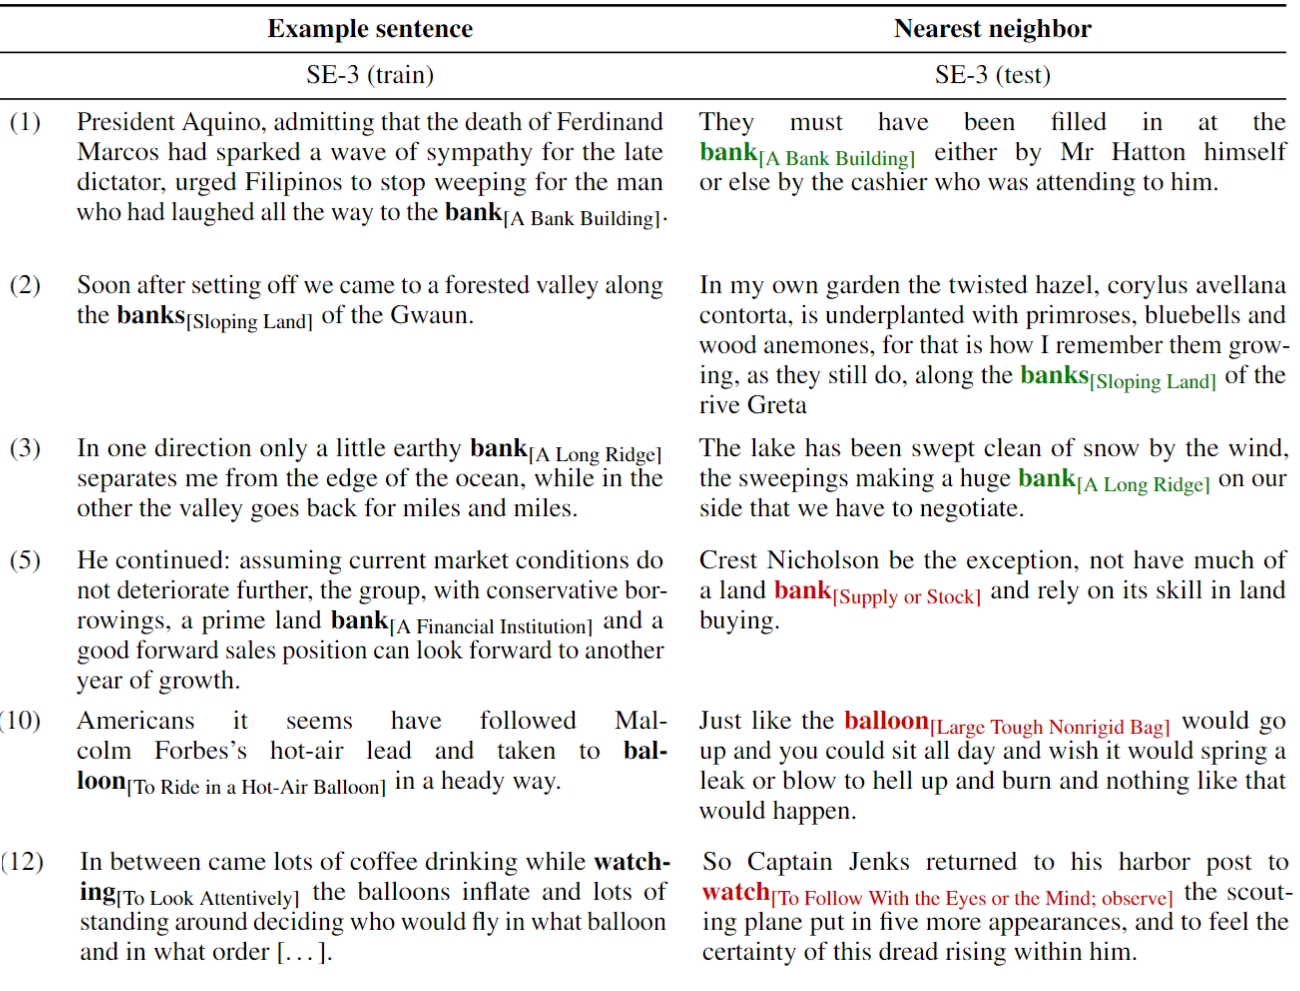
\includegraphics[width=\linewidth]{imgs/table_bertPolysemyTests.png}
    \end{minipage}
    
  \end{tabular}
  \label{tbl:bertPolysemy}
\end{table}



BERT did well when the data had \emph{vocabulary overlap} in context, such as in example (2) ``along the \emph{bank} of the river" (the input text) and `along the \emph{bank} of the river Greta" (nearest neighbor found by BERT). BERT also predicted correctly when text had \emph{semantic overlap}, such as in example (3)'s input ``little earthy bank" and nearest neighbor ``huge bank [of snow]". 

However, \emph{vocabulary and semantic overlap in conjunction} led BERT to make false predictions. Example (5) in \cref{tbl:bertPolysemy} shows BERT predicted ``land bank" as in a \emph{supply or stock} while the correct sense of ``land bank" was \emph{financial institution}. In example (10), the correct word sense of ``balloon" is a verb while BERT predicted a noun sense, so it did not even get the word class correct. Even harder for BERT was to distinguish verb senses correctly; example (12) shows the correct sense label of the \hyperref[sec:Polysemy]{polysemic} word ``watch" was \emph{to look attentively} while BERT's predicted sense was \emph{to follow with the eyes or the mind; observe}. 

Despite BERT's limitations, the authors conclude still that BERT captures \hyperref[sec:Polysemy]{polysemy} more successfully than \nameref{sec:ELMo}, inspiring future work in using \nameref{nlptask:wordsensedisambiguatioNWSD} to compare BERT to models like \nameref{sec:XLNet}. % done
\section{Transformer-XL} \label{sec:TransformerXL}

\subsection{Problem With Transformer: Context-Fragmentation Problem} \label{sec:ContextFragmentationProblem}


\begin{figure}[h]
\vspace{-5pt}
\centering
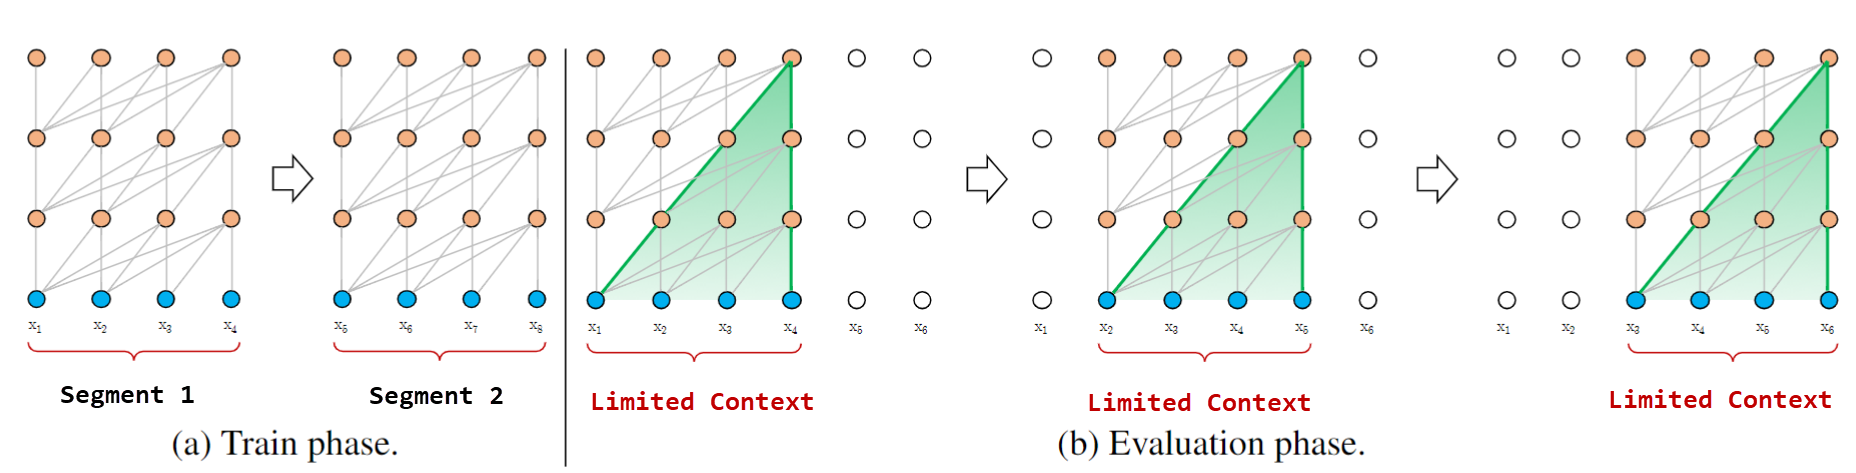
\includegraphics[width=\linewidth]{imgs/transXL_vanillaSegmentation.png}
%\vspace{-5pt}
\caption{Vanilla \nameref{sec:Transformer} with segment embedding length $ = 4$. During each evaluation step, the \nameref{sec:Transformer} consumes a segment embedding and makes a prediction at the last position. Next, the segment is shifted one position, so the new segment must be processed from scratch, \hyperref[sec:ContextFragmentationProblem]{breaking context dependency} between first tokens of each segment and between segments. From \emph{Transformer-XL: Attentive Language Models Beyond a Fixed-Length Context}, by Dai et al., 2019. \url{https://arxiv.org/pdf/1901.02860.pdf}. Copyright 2019 by Dai et al.}
%\vspace{-5pt}
\label{fig:transXL_VanillaSegment}
\end{figure}

\nameref{sec:Transformer}s cannot learn long-term dependencies because of {\label{sec:FixedLengthContext} \textbf{fixed-length context}}, or context that is limited by input length (Dai et al., 2019). The \emph{vanilla} (ordinary) \nameref{sec:Transformer} model adapted by Al-Rfou et al. (2018) uses fixed-length context since the model is trained within its segment embeddings, blocking information from flowing across segment embeddings during forward and backward propagation passes. %\hyperref[sec:ForwardProp]{forward} and \hyperref[sec:BackwardProp]{backward passes}. 
This result, visible in \cref{fig:transXL_VanillaSegment}, causes the \nameref{sec:Transformer} to forget context from previous segments. This is termed the \textbf{context fragmentation problem}.


\subsection{Motivation for Transformer-XL} \label{sec:MotivationForTransformerXL}

\textbf{Transformer-XL} (extra long) avoids ``disrupting temporal coherence." Instead of breaking up sequences into arbitrary \textbf{fixed lengths}, the Transformer-XL \emph{respects natural language boundaries} like sentences and paragraphs, helping it gain richer context over these and longer texts like documents. Through the use of \hyperref[sec:SegmentLevelRec]{segment-level recurrence mechanism} and \hyperref[sec:RelativePosEnc]{relative positional encoding}s, the Transformer-XL can overcome the \hyperref[sec:ContextFragmentationProblem]{context-fragmentation problem} and represent longer-spanning dependencies (Dai et al., 2019). 


\subsection{Describing Transformer-XL} \label{sec:DescribingTransformerXL}

\subsubsection{Segment-Level Recurrence Mechanism} \label{sec:SegmentLevelRec}

To resolve the \hyperref[sec:ContextFragmentationProblem]{context fragmentation problem}, the Transformer-XL employs a \textbf{segment-level recurrence mechanism} to capture long-term dependencies using information from previous segments. When a segment is being processed, each hidden layer receives two inputs: ($1$) the previous hidden layer outputs of the \emph{current segment} (akin to the vanilla model, shown as gray arrows in \cref{fig:transXL_extendedContext}), and ($2$) the previous hidden layer outputs of the \emph{previous segment} (green arrows in \cref{fig:transXL_extendedContext}). So although gradient updates or training still occurs within a segment, this extended context feature lets historical information to be fully used, avoiding \hyperref[sec:ContextFragmentationProblem]{context fragmentation}. 


\begin{figure}[h]
%\vspace{-5pt}
\centering
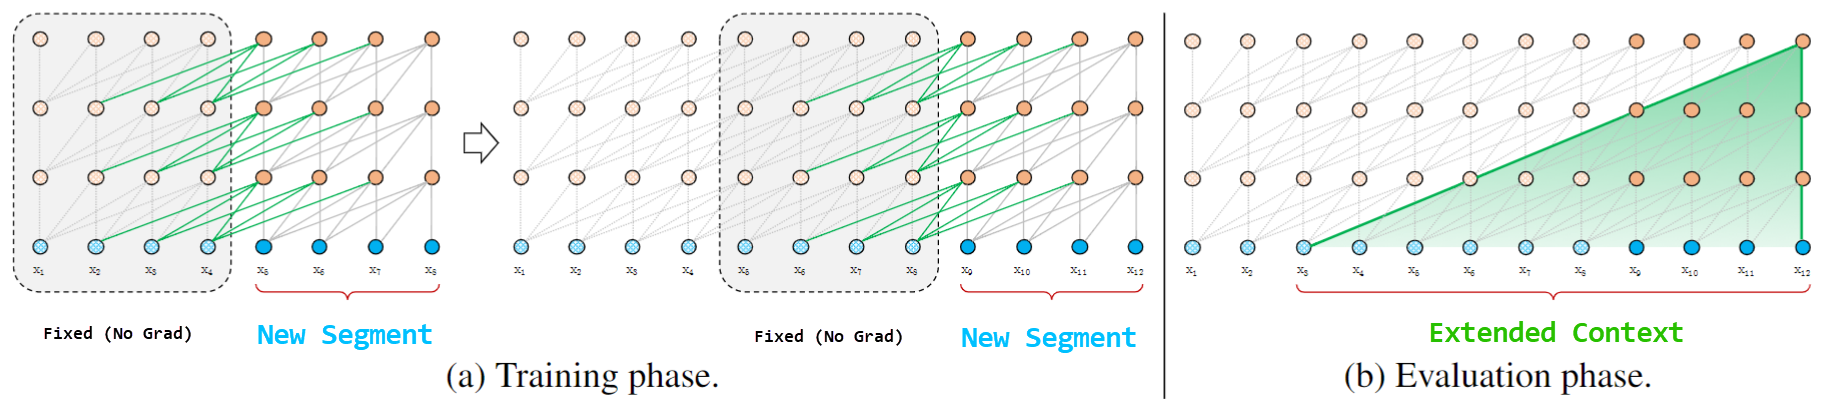
\includegraphics[width=\linewidth]{imgs/transXL_extendedcontext.png}
%\vspace{-5pt}
\caption{Segment level recurrence mechanism at work: the hidden state for previous segment is \emph{fixed} and \emph{stored} to later be reused as an extended context while the new segment is processed. Like in \nameref{sec:Transformer}, gradient updates or training still occurs within a segment, but the extended context feature allows historical information to now be incorporated. From \emph{Transformer-XL: Attentive Language Models Beyond a Fixed-Length Context}, by Dai et al., 2019. \url{https://arxiv.org/pdf/1901.02860.pdf}. Copyright 2019 by Dai et al.}
%\vspace{-20pt}
\label{fig:transXL_extendedContext}
\end{figure}


Intuitively, for the sentence ``I went to the store. I bought some cookies," the model receives the sentence ``I went to the store," caches the hidden states, and only \emph{then} feeds the remaining sentence ``I bought some cookies" and cached hidden states together into the model (Kurita, 2019b). 

To formally describe the recurrence mechanism, let $\textbf{s}_\tau = \Big\{ x_{\tau_1}, x_{\tau_2}, ..., x_{\tau_L} \Big\}$ and $\textbf{s}_{\tau + 1} = \Big\{ x_{{\tau+1}_1}, x_{{\tau+1}_2}, ..., x_{{\tau+1}_L} \Big\}$ denote two consecutive segment embeddings of length $L$. Let $\textbf{h}_\tau^n \in \mathbb{R}^{L \times d}$ be the $n$-th layer's hidden state vector produced for the $\tau$-th segment $\textbf{s}_\tau$, where $d$ is the hidden dimension. Then $n$-th layer's hidden state for next segment $\textbf{s}_{\tau + 1}$ is calculated in \cref{eq:TransXLHiddens} as:


\begin{equation}
\begin{array}{ll}
\Tilde{\textbf{h}}_{\tau + 1}^{n-1} = \Big\{ \texttt{StopGradient}\Big( \textbf{h}_\tau^{n-1} \circ \textbf{h}_{\tau+1}^{n-1} \Big) \Big\} \\\\
%
\textbf{q}_{\tau+1}^n, \;\;\; \textbf{k}_{\tau+1}^n, \;\;\; \textbf{v}_{\tau+1}^n = \textbf{h}_{\tau+1}^{n-1} \cdot \textbf{W}_q^T, \;\;\; \Tilde{\textbf{h}}_{\tau+1}^{n-1} \cdot \textbf{W}_k^T, \;\;\; \Tilde{\textbf{h}}_{\tau+1}^{n-1} \cdot \textbf{W}_v^T \\\\
%
\textbf{h}_{\tau+1}^n = \texttt{TransformerLayer} \Big( \textbf{q}_{\tau+1}^n, \;\;\; \textbf{k}_{\tau+1}^n \;\;\; \textbf{v}_{\tau+1}^n \Big)
\end{array}
\label{eq:TransXLHiddens}
\end{equation}



where the first line indicates that the two consecutive hidden states are concatenated; $\textbf{W}$ denotes model parameters; and $\textbf{q}, \textbf{k}, \textbf{v}$ are the \hyperref[sec:QKV]{query, key, and value vectors}. The key feature here, compared to standard \nameref{sec:Transformer}, is that the key $\textbf{k}_{\tau+1}^n$ and value $\textbf{v}_{\tau+1}^n$ are conditioned on the elongated context $\Tilde{\textbf{h}}_{\tau+1}^{n-1}$ \emph{and} the previous segment's cached context $\textbf{h}_\tau^{n-1}$. This is visible by the green lines in \cref{fig:transXL_extendedContext}.  

This new recurrence scheme allows more efficient computations. Also, it can cache multiple previous segments not just the previous one, making it more similar to an \hyperref[sec:RNN]{RNN's memory}. 




\subsubsection{Relative Positional Encoding} \label{sec:RelativePosEnc}

Trying to graft the \nameref{sec:Transformer}'s \hyperref[sec:PosEncodings]{positional encodings} directly with the \hyperref[sec:SegmentLevelRec]{segment-level recurrence mechanism} caused problems. Simply put, the Transformer-XL could not keep positional word order straight when reusing hidden states because tokens from different segments ended up with the same \hyperref[sec:PosEncodings]{positional encodings}, even though their position and importance could differ. This confused the model. 

To remedy this and correctly merge the recurrence scheme with positional word order, the authors invented \textbf{relative \hyperref[sec:PosEncodings]{positional encodings}} that work conjunction with \hyperref[sec:AttentionMechanism]{attention score}s of each layer, as opposed to only before the first layer, and which are based on \emph{relative} not \emph{absolute} distances between tokens (Horev, 2019). Formally speaking, the authors created a relative \hyperref[sec:PosEncodings]{positional encoding}s matrix whose $i$-th row indicates a relative distance of $i$ between two positions, and injected this into the attention module. As a result, the query vector can distinguish between two tokens using their different distances. Now, from Dai et al. and Horev (2019), the attention head calculation has four parts: 

\begin{enumerateSpaced}{3pt}
    \item \textbf{Content-based addressing: }the original attention score without \hyperref[sec:PosEncodings]{positional encoding}.
    
    \item \textbf{Content-dependent positional bias: }with respect to the current query. It uses a sinusoidal function that gets distance between tokens instead of \emph{absolute} position of a current token. 
    
    \item \textbf{Learned global content bias: } is a learned vector that accounts for the other tokens in the key matrix.
    
    \item \textbf{Learned global positional bias: }is a learned vector that adjusts the importance based only on distance between tokens, using the intuition that recent previous words are more relevant that a word from the previous paragraph. 
\end{enumerateSpaced}




\subsection{Experimental Results: Ablation Study for Segment-Level Recurrence and Relative Positional Encodings} \label{sec:ExpResultsTransXL}


% NOTE: secret to make text not overlap is either: 
% (1) enlarging the image just right
% (2) including all possible text after wrapfigure, not including few texts (as much text as possible within the parantheses).

{
\begin{wrapfigure}{L}{0.75\textwidth}
\begin{center}
    \vspace{-20pt}
    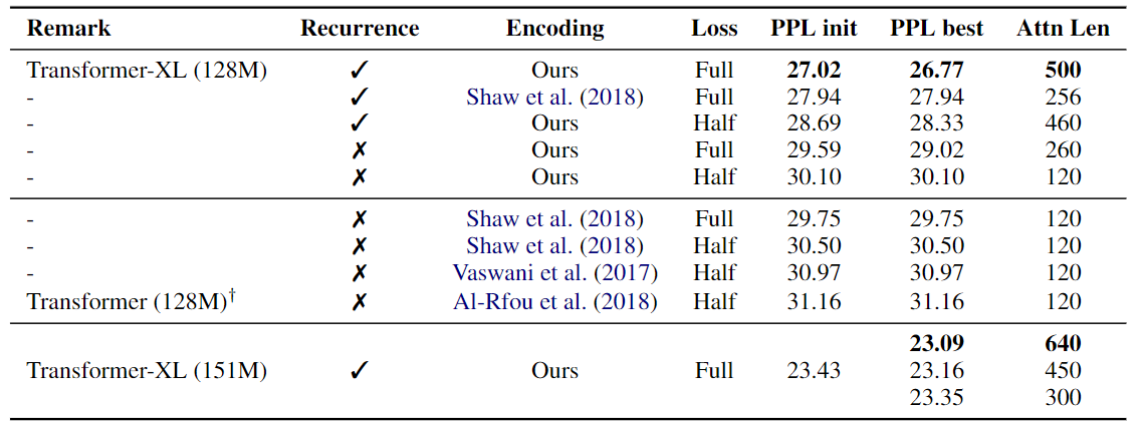
\includegraphics[width=\linewidth]{imgs/table_transXL_ablationREC.png}
\end{center}
\vspace{-20pt}
\captionof{table}{\scriptsize Ablation study for \nameref{sec:SegmentLevelRec} on the WikiText-103 data set. \textbf{PPL best} (model output) means perplexity score obtained using an optimal backpropagation %\hyperref[sec:BackwardProp]{backpropagation} 
training time length. \textbf{Attn Len} (model input) is the shortest possible attention length during evaluation to achieve the corresponding PPL best. From \emph{Transformer-XL: Attentive Language Models Beyond a Fixed-Length Context}, by Dai et al., 2019. \url{https://arxiv.org/pdf/1901.02860.pdf}. Copyright 2019 by Dai et al.}
\vspace{25pt}
\label{tbl:transXL_ablationRECURR}
\end{wrapfigure}

The authors seek to isolate the effects of Transformer-XL's \hyperref[sec:SegmentLevelRec]{segment-level recurrence mechanism} using with different encoding schemes. In \cref{tbl:transXL_ablationRECURR}, Shaw et al. (2018) uses relative encodings, and Vaswani and Al-Rfou use absolute encodings. 

In \cref{tbl:transXL_ablationRECURR}, \hyperref[sec:SegmentLevelRec]{segment-level recurrence} and \hyperref[sec:RelativePosEnc]{relative positional encoding} must be used in conjunction for best performance, since when using the new recurrence with the new encodings, the Transformer-XL can generalize to larger attention sequences (with length $500$) during evaluation while getting lowest perplexity score of $26.7$. 


However, if the Transformer-XL just uses the new encodings, even using shorter attention sequences of $260$ and $120$ with different backprop loss schemes cannot help lower its perplexity scores, as shown in the last two rows of \cref{tbl:transXL_ablationRECURR}'s Transformer-XL section. The standard \nameref{sec:Transformer} does poorly in general, showing high overall perplexities even using short attention lengths. 
}% done
\section{XLNet} \label{sec:XLNet}

While most commonly in NLP models are in the form of neural networks that are pretrained on large, unlabeled data and then fine-tuned for specific tasks, different unsupervised pretraining loss functions have also been explored. From these, \nameref{sec:autoregressiveLM} and \nameref{sec:autoencodingLM} have been the most powerful pretraining objectives. 


\subsection{Problems With BERT}

From Yang et al. (2020), a \emph{forward} \nameref{sec:autoregressiveLM} maximizes the likelihood of an input sequence by using a \emph{forward} autoregressive decomposition, shown in \cref{eq:AutoRegLMLoss}:

\begin{equation}
\textit{max}_\theta \Bigg( \textit{log}  \; P_\theta(\textbf{x})  \Bigg) = \sum_{t=1}^T \textit{log} \; P_\theta \Big(x_t \; | \; \textbf{x}_{< t} \Big)  
\label{eq:AutoRegLMLoss}
\end{equation}


Meanwhile, \nameref{sec:autoencodingLM}s like \nameref{sec:BERT} takes an input sequence $\textbf{x}$, and corrupts it $\hat{\textbf{x}}$ by masking some tokens. The autoencoding model recreates masked tokens $\overline{\textbf{x}}$ from the corrupted input $\hat{\textbf{x}}$, as in \cref{eq:AutoEncodeLMLOSS}:

\begin{equation}
\textit{max}_\theta \Bigg( \textit{log}  \; P_\theta(\overline{\textbf{x}} \; | \; \hat{\textbf{x}})  \Bigg) \;\; \mathlarger{\mathlarger{\approx}} \;\; \sum_{t=1}^T m_t \; \textit{log} \; P_\theta \Big(x_t \; | \; \hat{\textbf{x}} \Big) 
\label{eq:AutoEncodeLMLOSS}
\end{equation}

where $m_t = 1$ indicates that the input token $x_t$ is masked. With this in mind, Yang et al. (2020) note \nameref{sec:BERT}'s problems as follows: 

%\vspace{-10pt}

\begin{enumerateSpaced}{3pt}
    \item \textbf{Independence Assumption: } the $\approx$ approximation sign in \cref{eq:AutoRegLMLoss} indicates \nameref{sec:BERT} factorizes its joint conditional probability $P_\theta(\overline{\textbf{x}} \; | \; \hat{\textbf{x}})$ assuming that all masked tokens $\overline{\textbf{x}}$ are rebuilt independently of each other, even though texts are rife with long-range dependencies. 
    
    \item \textbf{Data Corruption}: Masking tokens from \nameref{sec:BERT}'s \hyperref[sec:maskedlanguagemodelMLM]{masked language modeling} task do not appear in real data during fine-tuning, and since \nameref{sec:BERT} does this in pre-training, a discrepancy arises between these two stages. 
\end{enumerateSpaced}


Kurita (2019b) gives an example to show how BERT predicts tokens independently. Consider the sentence: ``I went to the \texttt{[MASK]} \texttt{[MASK]} and saw the \texttt{[MASK]} \texttt{[MASK]} \texttt{[MASK]}."  Two ways to fill this are:  ($1$) ``I went to \emph{New York} and saw the \textit{Empire State building}," or ($2$) ``I went to \emph{San Francisco} and saw the \emph{Golden Gate bridge}." But \nameref{sec:BERT} might incorrectly mix things up and predict ``I went to \emph{San Francisco} and saw the \emph{Empire State building}." 

Clearly, since \nameref{sec:BERT} predicts masked tokens simultaneously, it fails to learn tokens' interlocking dependencies, which is a major point against \nameref{sec:BERT} since even simple \hyperref[sec:LanguageModels]{language models} learn at least unidirectional token dependencies (Kurita, 2019b). 




\subsection{Motivation for XLNet}

Confronted with \nameref{sec:BERT}'s limitations, Yang et al. (2020) conceived \textbf{XLNet} to keep the benefits of \emph{both} \hyperref[sec:autoencodingLM]{autoencoding} and \hyperref[sec:autoregressiveLM]{autoregressive} language modeling while avoiding their issue. Firstly, the \nameref{sec:autoregressiveLM} objective in XLNet lets the probability $P_\theta(\textbf{x))}$ (from \cref{eq:AutoRegLMLoss}) be factored using the universally-true probability product rule, side-stepping \nameref{sec:BERT}'s false independence assumption. Intuitively this means XLNet can predict tokens sequentially and autoregressively rather than simultaneously like \nameref{sec:BERT}. Secondly, XLNet's \textbf{\hyperref[sec:permutationLM]{permutation language model}} captures bidirectional context like an \hyperref[sec:autoencodingLM]{autoencoding model}. It uses a built-in \hyperref[sec:TwoStreamSelfAttention]{two-stream attention mechanism} to create target-aware predictions. 
 

\subsection{Describing XLNet}


\subsubsection{Permutation Language Model} \label{sec:permutationLM}

Can a model be trained to use \textbf{bidirectional context} while avoiding masking and its resulting problem of independent predictions? Like  \hyperref[sec:LanguageModels]{language model}s, a \textbf{permutation language model} predicts unidirectionally, but instead of predicting in order, the model predicts tokens in a random order. Simply put, a permutation language model must accumulate bidirectional context by finding dependencies between all possible input combinations (Yang et al., 2020). 

Consider the sentence: ``I like cats more than dogs." A traditional \hyperref[sec:LanguageModels]{language model} predicts individual words sequentially from previous context words. But a permutation language model randomly samples prediction order, such as: ``cats", ``than", ``I", ``more", ``dogs", ``like", where ``than" could be conditioned on ``cats" and ``I" might be conditioned on seeing ``cats, than", and so on (Kurita, 2019b). 



%\textbf{NOTE: } the permutation language model only permutes factorization order; it does not change word order in the input sequence, only the order in which words are predicted. XLNet still builds ``target-aware" predictions: input tokens can be fed in arbitrary order into XLNet using a masking feature in the \nameref{sec:Transformer}'s \hyperref[sec:AttentionMechanism]{attention} to temporarily cover certain tokens. Coupled with the use of \hyperref[sec:PosEncodings]{positional embeddings} and their associated original sequences, XLNet will still receive the tokens in correct order (Kurita, 2019b). This improves upon previous versions of permutation models which used an ``implicit position awareness" (Yang et al., 2020). 



\subsubsection{Need for Target-Aware Representations}\label{sec:TargetAwarePred}

Trying to merge \hyperref[sec:permutationLM]{permutation language model} and \nameref{sec:Transformer} blinded XLNet's target predictions to the permutation positions generated by the permutation language model. 

The fault lies in the nature of \nameref{sec:Transformer}s: while predicting a token at a position, \nameref{sec:Transformer} masks the token's embedding but \emph{unfortunately, also} its \hyperref[sec:PosEncodings]{positional encoding}, so it cannot see the position of the target it must predict. Intuitively, this means a sentence cannot be accurately represented, since positions like the beginning of a sentence have different distributions from other positions in the sentence. 

Formally, let $\mathcal{Z}_T =$ all possible permutations of the $T$-length sequence $\Big[1,2,...,T\Big]$; $\;\;\; z_t =$ the $t$-th element and $\textbf{z}_{< t} =$ the vector of the first $t-1$ elements of a permutation $\textbf{z} \in \mathcal{Z}_T$; $\;\;\; \textbf{x} =$ a text sequence of length $T$; $\;\;\; x_{z_t} =$ the content token to be predicted in the text sequence $\textbf{x}_{\textbf{z}_t}$ that is indexed by the permutations in $\textbf{z}_{< t}$. 

Yang et al. (2020) began by parameterizing the next-token predictive distribution using the softmax: 

\begin{equation}
P_\theta \Big( X_{z_t} = x_i\; | \; \textbf{x}_{\textbf{z}_t} \Big) = \frac{\exp {\Big( e(x_i)^T \cdot h_\theta \Big( \textbf{x}_{\textbf{z}_{< t}} \Big) \Big)}}  {\sum_{i=1} \exp{\Big( e(x_i)^T \cdot h_\theta \Big( \textbf{x}_{\textbf{z}_{< t}} \Big) \Big)}}
\label{eq:predDistNoTargetAware}
\end{equation}

where $e(x_i) =$ the embedding of the $i$-th token, $x_i$, and $h_\theta \Big( \textbf{x}_{\textbf{z}_{< t}} \Big) =$ the hidden state vector for $\textbf{x}_{\textbf{z}_t}$ created by the Transformer after masking. But $h_\theta \Big( \textbf{x}_{\textbf{z}_{< t}} \Big)$ does not depend on the position $z_t$ of the target it must predict, so XLNet is limited to predicting the same distribution regardless of target position. To remedy this, the authors replaced the hidden state $h_\theta$ in \cref{eq:predDistNoTargetAware} by $g_\theta \Big( \textbf{x}_{\textbf{z}_{< t}}, \; z_t \Big)$ which takes the target position $z_t$ as an argument. 




\subsubsection{Two-Stream Self-Attention }\label{sec:TwoStreamSelfAttention}

When formulating $g_\theta \Big( \textbf{x}_{\textbf{z}_{< t}}, \; z_t \Big)$ the \nameref{sec:Transformer} architecture produced yet another contradiction: ($1$) to predict token $x_{z_t}$, $g_\theta \Big( \textbf{x}_{\textbf{z}_{< t}}, \; z_t \Big)$ needs only the \emph{position} $z_t$ and not the \emph{content} $x_{z_t}$, or else the prediction becomes trivial, and ($2$) to predict all other tokens $x_{z_j}$ with $j > t$,  $g_\theta \Big( \textbf{x}_{\textbf{z}_{< t}}, \; z_t \Big)$ also needs $x_{z_t}$ to incorporate the entire contextual information. Thus, Dai et al. (2019) invented the \textbf{two-stream attention mechanism} which creates an overall hidden state from two separate sets of hidden states: the \textbf{content stream} and \textbf{query stream}.


The \textbf{content stream} $h_\theta \Big( \textbf{x}_{\textbf{z}_{\leq t}} \Big)$ encodes \emph{context} $\textbf{x}_{\textbf{z} \leq t}$ like ordinary hidden states in the \nameref{sec:Transformer}, while also encoding the \emph{content} token $x_{z_t}$. For the $t$-th prediction in the sentence, the content stream (using both $z_t$ and $x_{z_t}$) is computed for attention layers $m = 1, ..., M$ as $h_{z_t}^{(m)} = \texttt{Attention} \Big( \textbf{Q} = h_{z_t}^{(m-1)}, \;\; \textbf{KV} = \textbf{h}_{ {\color{cyan} \mathlarger{\mathlarger{\mathbf{z}_{\leq t}}}  } }^{(m-1)}; \;\; \theta  \Big)$.

% \begin{codeEnv}{python}
%     # Create permutation sequence: $\mathcal{Z}_T$
%     permutation = permute(range(T))
%     # Initialize content stream attention
%     h = [embeddings] + [Tensor(T) for _ in attentionLayers]
%     
%     for m, attention in enumerate(attentionLayers):
%         for t, position in enumerate(permutation):
%             # Including the current word (t) in the visible positions because of the $\textbf{h}_{ {\color{IndianRed} \mathlarger{\mathlarger{\mathbf{z}_{\leq t}}}  } }^{(m-1)}$
%             visiblePositions = permutation[:t+1]
%             # Content stream formula
%             h[m][position] = attention(queries = q[m-1][position], keys = h[m-1][visiblePositions], values = h[m-1][visiblePositions])
%     
% \end{codeEnv}
% \vspace{-20pt}
% \captionof{listing}{Content stream calculation}
% \label{code:ContentStreamAttn}
% \setlength{\parskip}{5pt}


\textbf{Query stream} $g_\theta \Big( \textbf{x}_{\textbf{z}_{< t}}, \; z_t \Big)$ encodes \emph{context} $\textbf{x}_{\textbf{z} \leq t}$ with \emph{position} $z_t$ simultaneously, but not the \emph{content} token $x_{z_t}$, to evade the contradiction. For the $t$-th prediction in a sentence, the query stream (using $z_t$ but not $x_{z_t}$) is computed as $g_{z_t}^{(m)} = \texttt{Attention} \Big( \textbf{Q} = g_{z_t}^{(m-1)}, \;\; \textbf{KV} = \textbf{h}_{ {\color{cyan} \mathlarger{\mathlarger{\mathbf{z}_{< t}}}  } }^{(m-1)}; \;\; \theta  \Big)$.


% \begin{codeEnv}{python}
%     # Create permutation sequence: $\mathcal{Z}_T$
%     permutation = permute(range(T))
%     # Compute the content stream as in above listing:
%     contentStrm = computeContentStream(permutation)
%     # Initialize query stream
%     q = [w] + [Tensor(T) for _ in attentionLayers]
%     
%     for m, attention in enumerate(attentionLayers):
%         for t, position in enumerate(permutation):
%             # Excluding the current word (t) in the visible positions because of the $\textbf{h}_{ {\color{IndianRed} \mathlarger{\mathlarger{\mathbf{z}_{< t}}}  } }^{(m-1)}$
%             visiblePositions = permutation[:t]
%             # Query stream formula
%             q[m][position] = attention(queries = q[m-1][position], keys = contentStrm[m-1][visiblePositions], values = contentStrm[m-1][visiblePositions])
%     
% \end{codeEnv}
% \vspace{-20pt}
% \captionof{listing}{Query stream calculation}
% \label{code:QueryStreamAttn}
% \setlength{\parskip}{5pt}
% %TODO: adding manual restoration of parskip here because it gets removed after the codesnippet - why? 


Intuitively, the purpose of the content and query stream is as follows. Suppose we must predict the word ``like" in \textit{``I like cats more than dogs"} where the previous words in the permutation were ``more" and ``dogs." The \textbf{content stream} would encode this information while the \textbf{query stream} would hold positional knowledge about ``like" as well as content stream information, so XLNet can predict ``like" (Kurita, 2019b). 



%\subsubsection{Using Transformer-XL}

%XLNet uses the \hyperref[sec:SegmentLevelRec]{segment-level recurrence mechanism} and \hyperref[sec:RelativePosEnc]{relative encodings}


\subsubsection{Relative Segment Encodings}\label{sec:RelativeSegmentEncodings}

XLNet builds on \nameref{sec:TransformerXL}'s \hyperref[sec:RelativePosEnc]{relative encodings} to model relationships between positions. While \nameref{sec:BERT} learns a segment embedding to distinguish \emph{which specific segments the (words) positions are from}, XLNet learns an embedding that encodes if two words are \emph{within the same segment embedding}. As a benefit, XLNet can be applied to tasks that take arbitrarily many input sequences (Kurita, 2019b).


\subsection{Conceptual Difference Between XLNet and BERT}
%\subsection{Experimental Results of XLNet}

To further illustrate the conceptual difference between XLNet and \nameref{sec:BERT} from a model training standpoint, take the list of words $\Big[ \texttt{New}, \texttt{York}, \texttt{is}, \texttt{a}, \texttt{city} \Big]$. Let the two tokens $\Big[ \texttt{New}, \texttt{York} \Big]$ be selected for prediction, so the models must maximize the log-likelihood: $\text{log} \; P(\texttt{New York} \; | \; \texttt{is a city})$. Assuming XLNet uses the factorization order $\Big[ \texttt{is}, \texttt{a}, \texttt{city}, \texttt{New}, \texttt{York} \Big]$, then \nameref{sec:BERT} and XLNet have the following loss functions: 

\begin{equation}
\begin{array}{ll}
\mathcal{J}_\text{BERT} = \text{log} \; P \Big( \texttt{New} \; | \; \texttt{is a city} \Big) \; + \; \text{log} \; P \Big( \texttt{York} \; | \; \texttt{is a city} \Big) \\
\mathcal{J}_\text{XLNet} = \text{log} \; P \Big( \texttt{New} \; | \; \texttt{is a city} \Big) \; + \; \text{log} \; P \Big( \texttt{York} \; | \; {\color{cyan} \texttt{New}}, \texttt{is a city} \Big) 
\end{array}
\label{eq:XLnetVsBERTLogLiks}
\end{equation}


While \nameref{sec:BERT} can learn some kind of dependency between the pairs \texttt{New} and \texttt{York}, \cref{eq:XLnetVsBERTLogLiks} clearly shows that XLNet learns stronger dependency or a ``denser training signal" (Dai et al., 2019). 

%For reading comprehension datasets like SQuAD and RACE where longer-context representation is required, XLNet outperformed \nameref{sec:BERT} as measured by their GLUE scores in \cref{tbl:xlnet_generalResults}.


% \begin{figure}[h]
% \vspace{-5pt}
% \centering
% 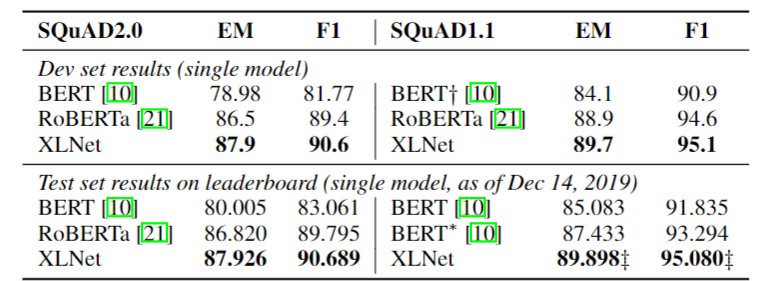
\includegraphics[width=0.7\textwidth]{imgs/xlnet_tableGeneralResults.png}
% \vspace{-5pt}
% \captionof{table}{\footnotesize Comparing GLUE scores of \nameref{sec:BERT} and BERT-based model called RoBERTa with XLNet. From \emph{Table 3 in XLNet: Generalized Autoregressive Pretraining for Language Understanding}, by Dai et al., 2019. \url{https://arxiv.org/pdf/1906.08237.pdf}. Copyright 2019 by Dai et al.}
% \vspace{-5pt}
% \label{tbl:xlnet_generalResults}
% \end{figure}


%Dai et al. (2019) used an ablation study to determine which component of XLNet is better than \nameref{sec:BERT}:  the \hyperref[sec:permutationLM]{permutation language model}, the \nameref{sec:TransformerXL} backbone, or some other details used in implementation, such as span-based prediction and next sentence prediction. The \cref{tbl:xlnet_ablationStudy} compares \nameref{sec:BERT}, \nameref{sec:TransformerXL}, and XLNet variations. Rows 1-4 show that \nameref{sec:TransformerXL} and the \hyperref[sec:permutationLM]{permutation language model} contribute to XLNet's success since its scores across different datasets are higher than for \nameref{sec:BERT}. Row 5 shows removing the memory caching reduces performance for the longer-context containing RACE data set. 

% 
% \begin{figure}[h]
% \vspace{-5pt}
% \centering
% 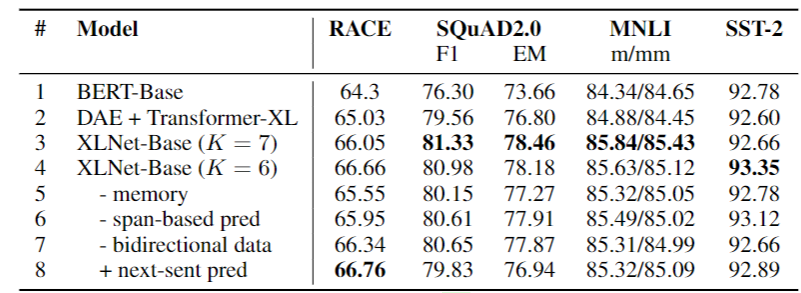
\includegraphics[width=0.7\textwidth]{imgs/xlnet_tableAblation.png}
% \vspace{-5pt}
% \captionof{table}{\footnotesize Ablation study for XLNet's \hyperref[sec:permutationLM]{permutation language model} on RACE, SQuAD, MNLI, SST-2 datasets. From \emph{Table 6 in XLNet: Generalized Autoregressive Pretraining for Language Understanding}, by Dai et al., 2019. \url{https://arxiv.org/pdf/1906.08237.pdf}. Copyright 2019 by Dai et al.}
% \vspace{-5pt}
% \label{tbl:xlnet_ablationStudy}
% \end{figure}
% 


%XLNet's integration of an \nameref{sec:autoregressiveLM} with \nameref{sec:TransformerXL} and a \hyperref[sec:TwoStreamSelfAttention]{two-stream attention mechanism} results in clear improvements over \hyperref[sec:maskedlanguagemodelMLM]{masked language models} like \nameref{sec:BERT}, which are prone to false assumptions and data corruption. 
\section{ERNIE 1.0} \label{sec:ERNIE_1}

\subsection{Motivation for ERNIE 1.0}

Previous models like \nameref{sec:Word2Vec}, \nameref{sec:Glove}, and \nameref{sec:BERT} create word vector representations only through surrounding contexts, not also through prior knowledge in the sentence, and thus fail to capture relations between entities in a sentence. Consider the following training sentence: 

{\large \textit{``Harry Potter is a series of fantasy novels written by J. K. Rowling."}}

Using co-occurring words ``J.", ``K.", and ``Rowling", BERT can is limited to predicting the token ``K." but utterly fails at recognizing the whole entity \emph{J. K. Rowling}. A model could use simple co-occurrence counts to predict the missing entity \emph{Harry Potter} even without using long contexts, but it would not be making use of the relationship between the novel name and its writer. 

Current NLP models analyzing simple word co-occurrence may miss additional information like sentence order and nearness and named entities. 



This is where \textbf{ERNIE} steps in. \textbf{ERNIE (Enhanced Representation through Knowledge Integration)} can extrapolate the relationship between the \emph{Harry Potter} entity and \emph{J. K. Rowling} entity using implicit knowledge of words and entities, and uses this relationship to predict that Harry Potter is a series written by J. K. Rowling (Sun et al., 2019a). 



%\begin{figure}[h]
%\vspace{-5pt}
%\centering
%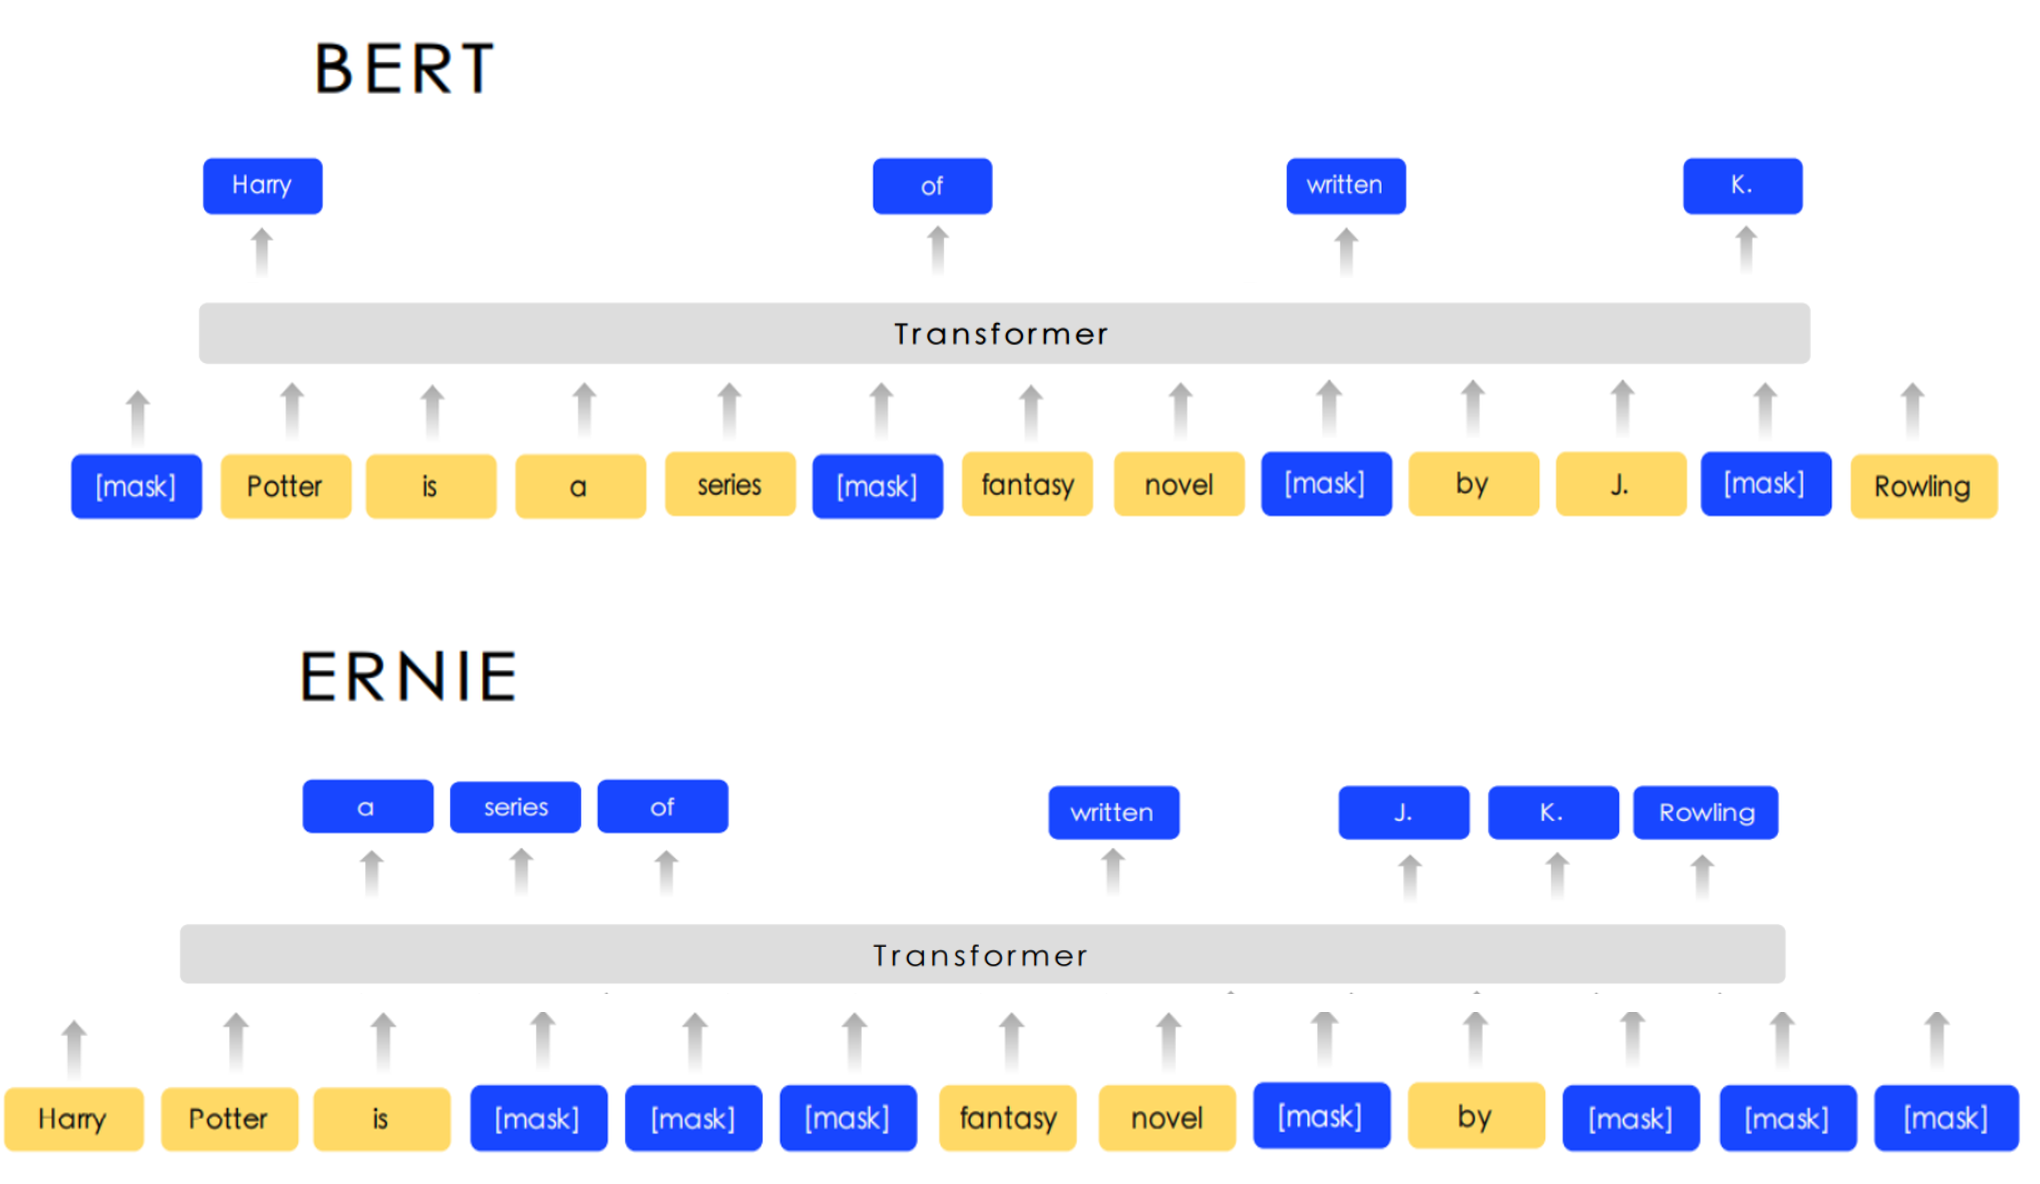
\includegraphics[width=0.9\textwidth]{imgs/ernie_vs_bert_masking.png}
%\vspace{-5pt}
%\captionof{figure}{\footnotesize Conceptual difference between \nameref{sec:BERT}'s masking and ERNIE's masking. From \emph{ERNIE: Enhanced Representation Through Knowledge Integration}, by Sun et al., 2019a. \url{https://arxiv.org/pdf/1904.09223.pdf}. Copyright 2019a by Sun et al.}
%\vspace{-5pt}
%\label{fig:ernie_vs_bert_masking}
%\end{figure}


ERNIE leverages a \nameref{sec:Transformer} encoder with \hyperref[sec:SelfAttention]{self-attention} alongside novel knowledge integration techniques like \nameref{sec:entitymasking} and \nameref{sec:phrasemasking} so that prior knowledge contained in conceptual units like phrases and entities can contribute to learning longer semantic dependencies for better model generalization and adaptability (Sun et al., 2019a). 


\subsubsection{phrase-level masking}\label{sec:phrasemasking}

A phrase is a ``small group of words of characters together acting as a conceptual unit" (Sun et al., 2019a). ERNIE uses lexical and chunking methods to determine phrase boundaries in sentences. In phrase-level masking, ERNIE randomly selects phrases from the sentences and masks them (as in \cref{fig:ernie_maskingTypes}), so that it can train by predicting the subpieces of the phrase. This way, phrase information can be built into ERNIE's learned word embeddings. 



\begin{figure}[h]
\vspace{-5pt}
\centering
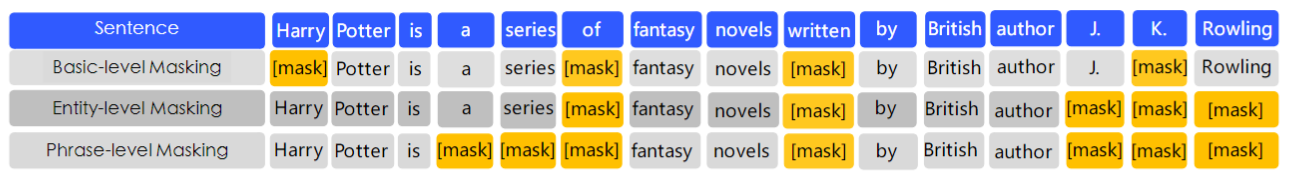
\includegraphics[width=0.99\textwidth]{imgs/ernie_maskingtypes.png}
\vspace{-5pt}
\captionof{figure}{\footnotesize ERNIE uses basic masking to get word representations, followed by phrase-level and entity-level masking. From \emph{ERNIE: Enhanced Representation Through Knowledge Integration}, by Sun et al., 2019a. \url{https://arxiv.org/pdf/1904.09223.pdf}. Copyright 2019a by Sun et al.}
\vspace{-5pt}
\label{fig:ernie_maskingTypes}
\end{figure}


\subsubsection{entity-level masking}\label{sec:entitymasking}

Sun et al. (2019a) say that name entities contain ``persons, locations, organizations, products" which can be denoted with a proper name, and can be abstract or have physical existence. Entities often contain important information within a sentence, so are regarded as conceptual units. ERNIE parses a sentence for its named entities, then masks and predicts all slots within the entities, as shown in \cref{fig:ernie_maskingTypes}.


\subsection{Experimental Results of ERNIE 1.0}\label{sec:ExperimentalResultsERNIE}





% NOTE: the top width must be +0.5 more than below textwidth measure
\begin{program}
\begin{wrapfigure}{L}{0.6\textwidth}
\begin{center}
    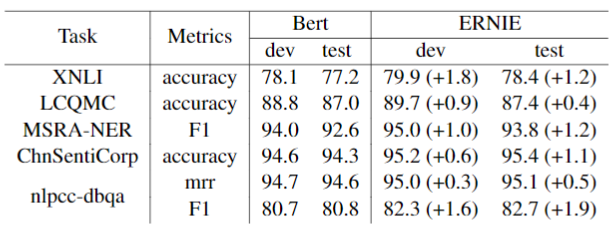
\includegraphics[width=0.55\textwidth]{imgs/ernie_tableResults.png}
\end{center}
\vspace{-20pt}
\captionof{table}{\footnotesize Comparing ERNIE and BERT on five major nlp tasks in Chinese. From \emph{Table 1 in ERNIE: Enhanced Representation Through Knowledge Integration}, by Sun et al., 2019a. \url{https://arxiv.org/pdf/1904.09223.pdf}. Copyright 2019a by Sun et al.}
\vspace{-5pt}
\label{tbl:ernie_vs_bert_Results}
\end{wrapfigure}

As in \cref{tbl:ernie_vs_bert_Results}, ERNIE outperforms \nameref{sec:BERT} by more than $1 \%$ absolute accuracy on five Chinese NLP tasks: \nameref{nlptask:naturallanguageinferenceNLI} (XNLI data), \nameref{nlptask:semantictextualsimilaritySTS} (LCQMC data), \nameref{nlptask:namedentityrecognitionNER} (MSRA-NER data), \nameref{nlptask:sentimentanalysisSA} (ChnSentiCorp data), \nameref{nlptask:questionansweringQA} (NLPCC-DBQA data).

\end{program}



Sun et al. assert this is because of ERNIE's knowledge integration masking strategies, and this is supported in \cref{tbl:ernie_ablationStudy}; adding phrase masking to basic word-level masking improved ERNIE's performance almost a full percent, and adding entity-level masking to this combination resulted in still higher gains when sampling more data from larger texts. 


\begin{figure}[h]
\vspace{-5pt}
\centering
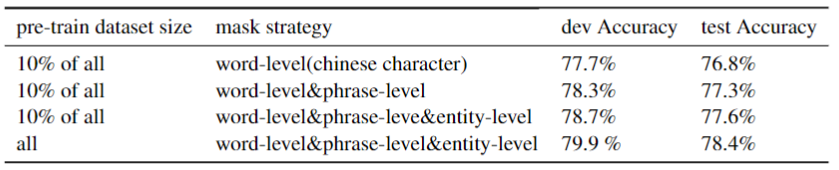
\includegraphics[width=0.8\textwidth]{imgs/ernie_tableAblation.png}
\vspace{-5pt}
\captionof{table}{\footnotesize Ablation study for ERNIE's \nameref{sec:phrasemasking} and \nameref{sec:entitymasking}. From \emph{Table 2 in ERNIE: Enhanced Representation Through Knowledge Integration}, by Sun et al., 2019a. \url{https://arxiv.org/pdf/1904.09223.pdf}. Copyright 2019a by Sun et al.}
\vspace{-5pt}
\label{tbl:ernie_ablationStudy}
\end{figure}



Additionally, the authors tested ERNIE's knowledge learning ability using fill-in-the-blanks on named entities in paragraphs. In case 1 from \cref{tbl:ernie_vs_bert_knowledgeLearningTask}, ERNIE predicts the correct father name entity based on prior knowledge in the article while \nameref{sec:BERT} simply memorizes one of the sons' name, completely ignoring any relationship between mother and son. In case 2, \nameref{sec:BERT} can learn contextual patterns to predict the correct named entity type but fails to fill the slot with the actual correct entity, while ERNIE fills the slots with the correct entity. In cases 3,4,6 \nameref{sec:BERT} fills the slots with characters related to the sentences but not with the semantic concept, while ERNIE again predicts the correct entities. 


\begin{table}[htbp]
\begin{tableFont}
    \small 
    \centering
    \setlength{\tabcolsep}{6pt} % Default value: 6pt
    %\cellspacetoplimit = 6pt\cellspacebottomlimit =6pt
    \renewcommand{\arraystretch}{2} % Default value: 1
    
    \begin{tabu} to \textwidth {| X[0.5] | X[7] | X | X | X |}
        
        \hline
  
        
        %\rowcolor{MyLavender} 
        \centering \textbf{Case}
        & \centering \textbf{Text} 
        & \centering \textbf{Predicted by ERNIE}\newline 
        & \centering\textbf{Predicted by BERT} 
        & \centering \textbf{Answer} \\ 
        
        \hline
        
        
        $1$
        &
        ``In September 2006, $\_\_\_$ married Cecilia Cheung. They had two sons, the older one is Zhenxuan Xie and the younger one is Zhennan Xie." \newline
        & 
        Tingfeng Xie
        & 
        Zhenxuan Xie
        & 
        {\color{Green} Tingfeng Xie} \\ 
        
        \hline 
        
        $2$
        &
        ``The Reform Movement of 1898, also known as the Hundred-Day Reform, was a bourgeois reform carried out by the reformists such as $\_\_\_$ and Qichao Liang through Emperor Guangxu."  \newline  
        & 
        Youwei Kang
        & 
        Schichang Sun
        & 
        {\color{Green} Youwei Kang} \\ 
        
        \hline 
        
        $3$
        &
        ``Hyperglycemia is caused by defective $\_\_\_$  secretion or impaired biological function, or both. Long-term hyperglycemia in diabetes leads to chronic damage and dysfunction of various tissues, generally eyes, kidneys, heart, blood vessels and nerves."   \newline 
        & 
        Insulin
        & 
        (Not a word in Chinese)
        & 
        {\color{Green} Insulin} \\ 
        
        \hline  
        
        $4$
        &
        ``Australia is a highly developed capitalist country with $\_\_\_$ as its capital. As the most developed country in the Southern Hemisphere, the $12$th largest economy in the world and the fourth largest exporter of agricultural products in the world, it is also the world's largest exporter of various minerals."   \newline 
        & 
        Melbourne
        & 
        (Not a city name)
        & 
        {\color{Green} Canberra} \\ 
        
        \hline 
        
        $6$
        &
        ``Relativity is a theory about space-time and gravity, which was founded by $\_\_\_$."   \newline 
        & 
        Einstein
        & 
        (Not a word in Chinese)
        & 
        {\color{Green} Einstein} \\ 
        
        
        \hline 
        
    \end{tabu}
    
    \captionof{table}{\footnotesize Comparing ERNIE to BERT on Cloze Chinese Task. From \emph{Figure 4 in ERNIE: Enhanced Representation Through Knowledge Integration}, by Sun et al., 2019a. . Copyright 2019a by Sun et al.}
    
    \label{tbl:ernie_vs_bert_knowledgeLearningTask}
\end{tableFont}
\end{table}




However in case 4, ERNIE predicts the wrong city name, though it still understands the semantic type. It is evident that ERNIE's contextual knowledge understanding is far superior to \nameref{sec:BERT}'s predictions (Sun et al., 2019a). 





% ------------------------------------------------------------

\section{ERNIE 2.0} \label{sec:ERNIE_2}


\subsection{Motivation for ERNIE 2.0}

Models such as \nameref{sec:Word2Vec}, \nameref{sec:Glove}, and \nameref{sec:BERT} extract meaning using co-occurrences. Even \nameref{sec:XLNet}'s permutation language model relies on co-occurrences. 


\begin{figure}[h]
\vspace{-5pt}
\centering
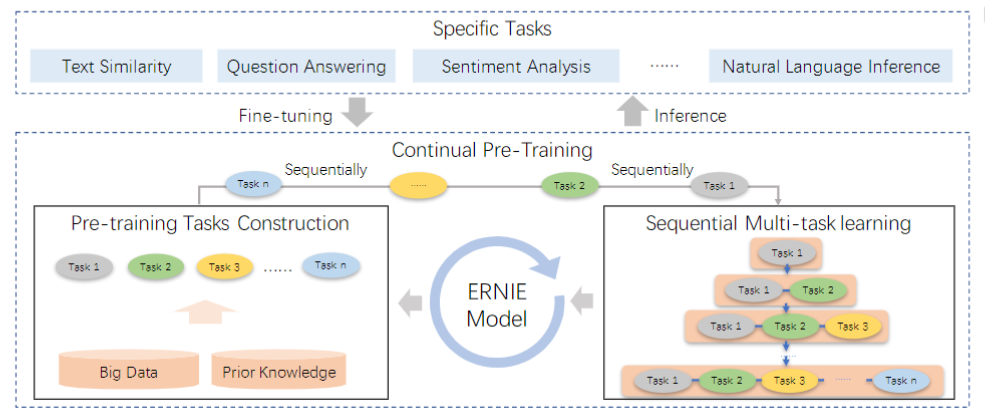
\includegraphics[width=0.9\textwidth]{imgs/ernie2_framework.png}
\vspace{-5pt}
\captionof{figure}{\footnotesize ERNIE 2.0's framework where embeddings are created by continual multi-task learning and then fine-tuned for specific \hyperref[app:Appendix_NLPTasks]{nlp tasks}. From \emph{Figure 1 in ERNIE 2.0: A Continual Pre-Training Framework for Language Understanding}, by Sun et al., 2019. \url{https://arxiv.org/pdf/1907.12412.pdf}. Copyright 2019 by Sun et al.}
\vspace{-5pt}
\label{fig:ernie2_framework}
\end{figure}


However, ERNIE 2.0 instead broadens the vision to more than just simple co-occurrence counts. Using a \hyperref[sec:ContinualMultiTaskLearning]{continual multi-task learning} framework (\cref{fig:ernie2_framework}) to remember previously learned knowledge, ERNIE 2.0 can capture ``lexical, syntactic and semantic information from training corpora in form of named entities (like person names,
location names, and organization names), semantic closeness (proximity of sentences),
sentence order or discourse relations” (Sun et al., 2019b).

\subsection{Continual Multi-Task Learning}\label{sec:ContinualMultiTaskLearning}

Inspired by human's ability to continuously accumulate information from past experience to develop new skills, \textbf{continual learning} (Parisi et al. 2019; Chen and Liu, 2018) trains a model sequentially in multiple tasks so that it remembers previously-learned tasks while learning new ones (Sun et al., 2019b). Humans do not forget skating when learning how to ski; continual learning helps a model do likewise. 


\begin{program}
\begin{wrapfigure}{L}{0.7\textwidth}
\begin{center}
    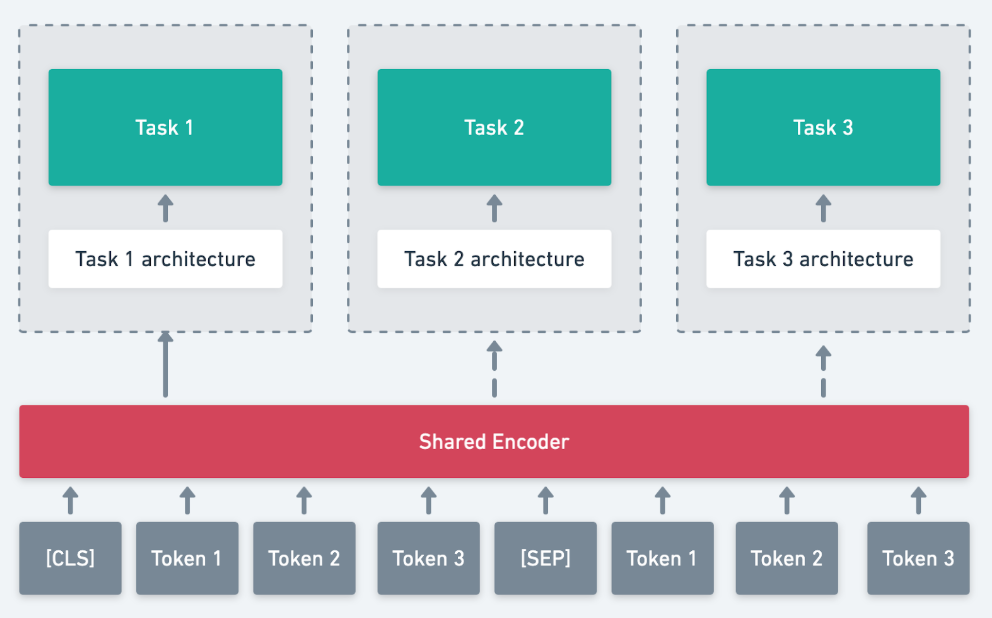
\includegraphics[width=0.6\textwidth]{imgs/multitaskExample.png}
\end{center}
%\vspace{-10pt}
\captionof{figure}{\footnotesize Example of multi-task learning. From \emph{ERNIE 2.0: A CONTINUAL PRE-TRAINING FRAMEWORK FOR LANGUAGE UNDERSTANDING}, by Sequeira, 2019. \url{https://medium.com/psyai/ernie-2-0-an-article-to-hopefully-answer-all-your-questions-b5df21a64090}. Copyright n.d. by n.d.}
%\vspace{-5pt}
\label{fig:multitaskexample}
\end{wrapfigure}

\textbf{Multi-task learning} means learning multiple tasks simultaneously. An example is in \cref{fig:multitaskexample} where an Encoder is shared across task-specific architectures. In multitask model training, data is batched and allocated for specific task training. All tasks take turns learning on their mini-batched data then separately update the shared encoder based on the loss. However, this separate, individual task learning affects the weights in the shared encoder, causing ``catastrophic forgetting" (Sequeira, 2019). 

\end{program}




\begin{program}
\begin{wrapfigure}{L}{0.7\textwidth}
    \centering
    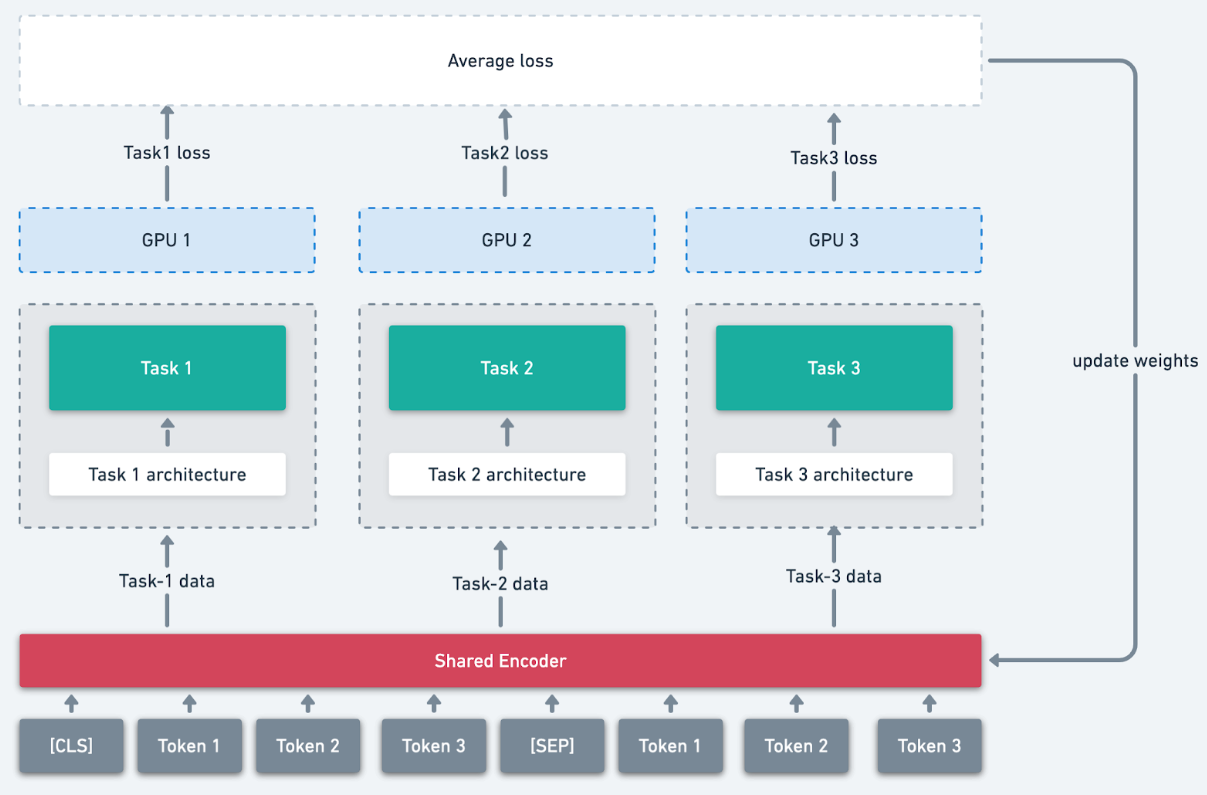
\includegraphics[width=0.65\textwidth]{imgs/ernie_continualMultitask.png}
%\end{center}
\vspace{-5pt}
\captionof{figure}{\footnotesize Continual multi-task learning in ERNIE. From \emph{ERNIE 2.0: A CONTINUAL PRE-TRAINING FRAMEWORK FOR LANGUAGE UNDERSTANDING}, by Sequeira, 2019. \url{https://medium.com/psyai/ernie-2-0-an-article-to-hopefully-answer-all-your-questions-b5df21a64090}. Copyright n.d. by n.d.}
\vspace{-10pt}
\label{fig:ernie_continualMultitaskLearning}
\end{wrapfigure}

ERNIE 2.0 however combines these two features into \textbf{continual multi-task learning}; several tasks are trained in parallel and the shared encoder is updated using the average of losses from all tasks. This is shown in \cref{fig:ernie_continualMultitaskLearning}. Specifically, for the first step, only Task 1 is learned and the encoder weights are updated from Task 1's loss. In step 2, the shared encoder is initialized with weights from the previous step and Task 1 and 2 are learned at the same time. Since the shared encoder has already learned from Task 1, only the loss from Task 2 will mostly updated the shared encoder, while retaining Task 1 information. Next, average loss is calculated to update the shared encoder. These steps continue until the model has trained on all tasks (Sequeira, 2019). 

\end{program}



\section{Discussion, Conclusion, and Future Work}\label{sec:ConcludeAndFuture}

\begin{itemize}
\item summarize what was written
-> machine translation (MT)
Did not expect this to be directly useful to my long term purpose of concept extraction (ml) but a good source of implementations
-> .... summarize

\item indicate future work directions
-> bayes polysemy
-> different representations: knowledge graph embeddings
-> model fine-tuning, transfer learning, domain adaptation for easier use.
-> more research into concept embeddings and key phrase extraction. 
\end{itemize}
\section*{References}\label{sec:References}

\vspace{10pt}

\begin{enumerateSpaced}{4pt}

    \item Smith, and A., N. (2019, February 19). Contextual Word Representations: A Contextual Introduction. Retrieved from \url{https://arxiv.org/abs/1902.06006}

    \item Melamud, O., Goldberger, et al. (2016). context2vec: Learning Generic Context Embedding with Bidirectional LSTM. \emph{Proceedings of The 20th SIGNLL Conference on Computational Natural Language Learning}. doi: 10.18653/v1/k16-1006
    
    \item Devlin, Jacob, et al. (2019, May 24). BERT: Pre-training of Deep Bidirectional Transformers for Language Understanding. Retrieved from \url{https://arxiv.org/abs/1810.04805}
    
    \item Wiedemann, Gregor, et al. (2019, September 23). Does BERT Make Any Sense? Interpretable Word Sense Disambiguation with Contextualized Embeddings. Retrieved from \url{https://arxiv.org/abs/1909.10430v1}
    
    \item Munikar, M., et al. (2019). Fine-grained Sentiment Classification using BERT. 2019 \emph{Artificial Intelligence for Transforming Business and Society (AITB)}. doi: 10.1109/aitb48515.2019.8947435
    
    \item Clark, K., et al. (2019). What Does BERT Look at? An Analysis of BERT’s Attention. \emph{Proceedings of the 2019 ACL Workshop BlackboxNLP: Analyzing and Interpreting Neural Networks for NLP}. doi: 10.18653/v1/w19-4828
    
    \item Ethayarajh, K. (2019). How Contextual are Contextualized Word Representations? Comparing the Geometry of BERT, ELMo, and GPT-2 Embeddings. \emph{Proceedings of the 2019 Conference on Empirical Methods in Natural Language Processing and the 9th International Joint Conference on Natural Language Processing (EMNLP-IJCNLP).} doi: 10.18653/v1/d19-1006

    \item Batista, D. (n.d.). Language Models and Contextualised Word Embeddings. Retrieved from \url{http://www.davidsbatista.net/blog/2018/12/06/Word_Embeddings/}
    
    \item Neelakantan, A., et al. (2014). Efficient Non-parametric Estimation of Multiple Embeddings per Word in Vector Space. \emph{Proceedings of the 2014 Conference on Empirical Methods in Natural Language Processing (EMNLP).} doi: 10.3115/v1/d14-1113
    
    \item Antonio, M. (2019, September 5). Word Embedding, Character Embedding and Contextual Embedding in BiDAF - an Illustrated Guide. Retrieved from \url{https://towardsdatascience.com/the-definitive-guide-to-bidaf-part-2-word-embedding-character-embedding-and-contextual-c151fc4f05bb}
    
    \item Mikolov, T., Sutskever, I., et al. (2013a, October 16). Distributed Representations of Words and Phrases and their Compositionality. Retrieved from \url{https://arxiv.org/pdf/1310.4546.pdf}
    
    \item Mikolov, Tomas, et al. (2013b, September 7). Efficient Estimation of Word Representations in Vector Space. Retrieved from \url{https://arxiv.org/abs/1301.3781}
    
    \item Weng, L. (2017, October 15). Learning Word Embedding. Retrieved from \url{https://lilianweng.github.io/lil-log/2017/10/15/learning-word-embedding.html}


    \item Pennington, J., Socher, R., and Manning, C. (2014). Glove: Global Vectors for Word Representation.\emph{Proceedings of the 2014 Conference on Empirical Methods in Natural Language Processing (EMNLP)}.doi: 10.3115/v1/d14-1162

    
    \item Kurita, K. (2018a, May 4). Paper Dissected: "Glove: Global Vectors for Word Representation" Explained. Retrieved from \url{http://mlexplained.com/2018/04/29/paper-dissected-glove-global-vectors-for-word-representation-explained/}
    
    \item Sutskever, I., et al. (2014, December 14). Sequence to Sequence Learning with Neural Networks. Retrieved from \url{https://arxiv.org/abs/1409.3215}
    
    \item Vaswani, Ashish, et al. (2017, December 6). Attention Is All You Need. Retrieved from \url{https://arxiv.org/abs/1706.03762}
    
    \item G, R. (2019, March 18). Transformer Explained - Part 1. Retrieved from \url{https://graviraja.github.io/transformer/}
    
    \item Ta-Chun. (2018, October 3). Seq2seq pay Attention to Self Attention: Part 1. Retrieved from \url{https://medium.com/@bgg/seq2seq-pay-attention-to-self-attention-part-1-d332e85e9aad}
    
    \item Alammar, Jay. “Visualizing A Neural Machine Translation Model (Mechanics of Seq2seq Models With Attention).” \emph{Visualizing A Neural Machine Translation Model (Mechanics of Seq2seq Models With Attention) – Jay Alammar – Visualizing Machine Learning One Concept at a Time}, 2018a, \url{jalammar.github.io/visualizing-neural-machine-translation-mechanics-of-seq2seq-models-with-attention/}.
    
    \item Alammar, J. (2018b, June 27). The Illustrated Transformer. Retrieved from \url{http://jalammar.github.io/illustrated-transformer/}


    \item Peters, et al. “Deep Contextualized Word Representations.” \emph{ArXiv.org}, (22 Mar. 2018), \url{arxiv.org/abs/1802.05365}.
    
    \item Dai, Zihang, et al. “Transformer-XL: Attentive Language Models beyond a Fixed-Length Context.” \emph{Proceedings of the 57th Annual Meeting of the Association for Computational Linguistics}, (2019), \url{https://arxiv.org/pdf/1901.02860.pdf}.
    
    \item Yang, Z, et al. "XLNet: Generalized Autoregressive Pretraining for Language Understanding." \emph{Proceedings of the 57th Annual Meeting of the Association for Computational Linguistics}, (2020), \url{https://arxiv.org/pdf/1906.08237.pdf}.
    
    \item Kurita, Keita. “Paper Dissected: ‘XLNet: Generalized Autoregressive Pretraining for Language Understanding’ Explained.” \emph{Machine Learning Explained}, (7 July 2019b), \url{mlexplained.com/2019/06/30/paper-dissected-xlnet-generalized-autoregressive-pretraining-for-language-understanding-explained/}.
    
    
    \item Sun, Y, et al. "ERNIE: Enhanced Representations Through Knowledge Integration." \emph{Proceedings of the 57th Annual Meeting of the Association for Computational Linguistics}, (2019a), \url{https://arxiv.org/pdf/1904.09223.pdf}.
    
    \item Sun, Y, et al. "ERNIE 2.0: A Continual Pre-Training Framework for Language Understanding." \emph{Proceedings of the 57th Annual Meeting of the Association for Computational Linguistics}, (2019b), \url{https://arxiv.org/pdf/1907.12412.pdf}.
    
\end{enumerateSpaced}
    

\appendix
\clearpage 
\section{APPENDIX: Glossary of NLP Tasks} \label{app:Appendix_NLPTasks}

Most of these definitions are from Collobert et al. (2011). 


\subsection{semantic parsing (SP)} \label{nlptask:semanticparsingSP}

\textbf{Semantic parsing (SP)} converts a natural language representation into machine-understanding form. Types include \nameref{nlptask:machinetranslationMT} and \nameref{nlptask:questionansweringQA}.


\subsection{key phrase extraction} \label{nlptask:keyphraseextraction}

\textbf{Key phrase extraction} task uses morphological,  syntactic information, and typed grammar dependencies to learn relevant phrases, and is an important tool for concept extraction. Systems may use \nameref{nlptask:postagging} and \nameref{nlptask:namedentityrecognitionNER} and \nameref{nlptask:namedentityrecognitionNER} to recognize that \texttt{``Air Canada"} is a single entity composed of separate words which only when combined give new meaning (Mikolov et al., 2013a). In some cases, \nameref{nlptask:postagging} uses noun phrases to extract key phrases. 

Key phrase extraction is used in the real world to automate data collection; it results in benefits like data scalability and consistent criteria, so concepts can become used and interlinked at fine-grained levels (``Keyword Extraction", 2019). 



\subsection{machine translation (MT)} \label{nlptask:machinetranslationMT}

\textbf{Machine translation (MT)} task translates an input text in a given language to a target language. There are many population neural translation models like the \nameref{sec:Seq2Seq} and \nameref{sec:BERT} that use the \hyperref[sec:AttentionMechanism]{attention mechanism} to account for contextual meaning across a sentence and not just translate word by word. 

\subsection{neural machine translation (NMT)} \label{nlptask:neuralmachinetranslationNMT}

\textbf{Neural machine translation (NMT)} is \nameref{nlptask:machinetranslationMT} applied in \nameref{sec:NeuralLM}s. 


\subsection{question answering (QA)} \label{nlptask:questionansweringQA}

\textbf{Question answering (QA)} is a task for machines to answer questions posed by humans in a natural language. 


\subsection{semantic role labeling (SRL)} \label{nlptask:semanticrolelabelingSRL}

Also called ``shallow" \nameref{nlptask:semanticparsingSP} , \textbf{semantic role labeling (SRL)} is often described as answering the question ``Who did what to whom?" (Peters et al. 2018). It tries to give a semantic role or tag to a syntactic constituent of a sentence (Collobert et al., 2011).  Examples of semantic roles are \emph{agent, goal} or \emph{result}. 

Specifically, it detects semantics associated to a syntactic sentence feature like predicate or verb and then assigns them semantic roles. 
\begin{itemize}
    \item \textbf{Example Input Sentence: } ``Mary sold the book to John."
    
    \item \textbf{Example Output: } for the verb $\Big[ \text{"to sell"}\Big]_\text{predicate}$; for the noun or argument $\Big[ \text{"Mary"}\Big]_\text{agent}$; for the noun $\Big[ \text{"the book"}\Big]_\text{goods (theme)}$; for the noun $\Big[ \text{"John"}\Big]_\text{recipient}$.
\end{itemize}

SRL can give multiple labels depending on the usage of the syntactic constituent in the sentence. 



\subsection{named entity recognition (NER)} \label{nlptask:namedentityrecognitionNER}

\textbf{Named entity recognition (NER)} is a kind of information extraction task that labels known entities in text into categories like ``Person", ``Location," and ``Organization." \newline 

An \textbf{entity} is a proper noun such as a person, place, or product. A proper noun is more specific than general nouns, which represent more ambigious concepts; for example, ``Emma Watson", ``Eiffel Tower" and ``Second Cup" are entites but the corresponding nouns ``actress", ``architecture" and ``store" are themes.



\subsection{named entity disambiguation (NED)} \label{nlptask:namedentitydisambiguationNED}

\textbf{Named entity disambiguation (NED)} or \textbf{entity linking (EL)} links or maps mentions of an entity (such as persons, locations, companies) within a text to corresponding unique entities in a knowledge base (Shahbazi et al., 2019). 

\begin{itemize}
    \item \textbf{Example input text: } ``Jordan as a  member of the Tar Heels' national championship team."
    
    \item \textbf{Example output: } the language model should predict the named entity (person) ``Michael Jordan", given this exists in the knowledge base, rather than the ambigious mention ``Jordan". 
\end{itemize}

%\subsection{entity extraction (EE)} \label{nlptask:entityextraction}

%\subsection{entity typing (ET)} \label{nlptask:entitytypingET}



\subsection{part of speech tagging (POS)} \label{nlptask:postagging}

\textbf{Part-of-speech tagging (POS)} is the process of labeling each word in a sentence with its part of speech. Every word token is labeled with a tag that identifies its syntactic role (noun, verb, advergb, adjective, ...).  

From (Mohler, 2019): 

\begin{itemize}
    \item \textbf{Example Input Sentence: } ``The tall man is going to quickly walk under the ladder."
    
    \item \textbf{Example Output: } $\Big[ \text{"man"}\Big]_\text{Noun}$, \ $\Big[ \text{"walk"}\Big]_\text{Verb}$, \ $\Big[ \text{"ladder"}\Big]_\text{Noun}$, \ $\Big[ \text{"quickly"}\Big]_\text{Adverb}$ and so on. 
\end{itemize}




\subsection{chunking} \label{nlptask:chunking}

\textbf{Chunking} labels entire pieces of a sentence with tags that indicate their part of speech or syntactic role. For example a phrase can be labeled \emph{noun phrase (NP)}, or \emph{verb phrase (VP)} or even \emph{begin-chunk (B-NP)} and \emph{inside-chunk (I-NP)}. Each \emph{phrase} token is assigned one distinct part of speech tag. 

Chunking operates on the \emph{phrase level} while \nameref{nlptask:postagging} operates on the \emph{word level}. 

From (Mohler, 2019): 
\begin{itemize}
    \item \textbf{Example Input Sentence: } ``The tall man is going to quickly walk under the ladder."
    
    \item \textbf{Example Output: } $\Big[ \text{"the tall man"}\Big]_\text{Noun Phrase}$, \ $\Big[ \text{"is going to quickly walk"}\Big]_\text{Verb Phrase}$, \\ $\Big[ \text{"under the ladder"}\Big]_\text{Preopositional Phrase}$.
\end{itemize}




\subsection{word sense disambiguation (WSD)} \label{nlptask:wordsensedisambiguatioNWSD}

\textbf{Word sense disambiguation (WSD)} identifies the correct word usage from a collection of senses. For a sentences containing \hyperref[sec:Polysemy]{polysemous words}, models use contextual evidence to determine the correct word sense. 



\subsection{lexical substitution} \label{nlptask:lexicalsubstitution}

\textbf{Lexical substitution} substitutes a word given its contextual meaning. For example, the word ``bright" in the phrase ``bright child" can be replaced with ``smart" or ``gifted" rather than ``shining" (Brazinkas et al., 2018). 

\subsection{entailment recognition (ER)} \label{nlptask:entailmentrecognition}

The \textbf{entailment recognition} task is a kind of lexical entailment task or hyponymy detection. Given a pair of words, the task is to predict if the first word $w_1$ entails the second one $w_2$. For (``kiwi", ``fruit"), the task would be to confirm that ``kiwi" entails ``fruit" since it is its hyponym. 


\subsection{textual entailment (TE)} \label{nlptask:textualentailmentTE}

\textbf{Textual entailment (TE)} is the task of determining if a ``hypothesis" is true given a ``premise" (Peters et al., 2018). 

\subsection{entailment directionality prediction} \label{nlptask:entailmentdirectionalityprediction}

Given a pair of words, the \textbf{entailment directionality prediction} task must predict if the previous word entails the next one, or vice versa. It is known that entailment holds for the given word pair and only its directionality is being predicted (Brazinkas et al., 2018). 

\subsection{sentiment classification (SC)} \label{nlptask:sentimentclassificationSC}

See \nameref{nlptask:sentimentanalysisSA}.

\subsection{sentiment analysis (SA)} \label{nlptask:sentimentanalysisSA}

\textbf{Sentiment analysis (SA)} evaluates the sentiment expressed towards an entity (noun or pronoun) based on its proximity to positive or negative words (adjectives and adverbs). For example, a model may classify a movie review as positive, negative or neutral. Generally, SA systems find several attributes of the expression alongside its \emph{polarity}, including the \emph{subject}, the thing being talked about, and \emph{opinion holder}, the entity holding the opinion. 

This task may assign weighted sentiment values to the entities and themes within text. For instance, a hotel getting a review ``astonishing scenery" would get a higher sentiment score than ``banal lake view" because of the stronger adjective ``astonishing." 


\subsection{word similarity} \label{nlptask:wordsimilarity}

The \textbf{word similarity} task determines a similarity score for two input texts. Numerical measures such as cosine similarity compute angular distance between words, based on textual evidence. 


\subsection{word analogy} \label{nlptask:wordanalogy}

The \textbf{word analogy} task completes an analogy. For instance, given the analogy ``meteor" is to ``sky" as ``dolphin" is to <blank>, the task would be to predict a word representing a body of water. 


\subsection{coreference resolution (CR)} \label{nlptask:coreferenceresolutionCR}

\textbf{Coreference resolution (CR)} is the task of collecting all expressions in a text that refer to the same entity in a text.  that refer to the same underlying real world entities. 

\begin{itemize}
    \item \textbf{Example input text: } ``The monkey clambered up the baobab tree and he grabbed a banana and ate it there. The hairy ape screeched while watching the setting sun over the river."
    
    \item \textbf{Example output: } tag the coreferent phrases ``he" and ``the hairy ape" with  ``the monkey"; and also tag ``it" with the same label as ``banana." 
    
\end{itemize}

This task is used as a step towards more general tasks, and is not an end-user task. 

\subsection{sequence labeling (SL)} \label{nlptask:sequencelabelingSL}

\textbf{Sequence labeling (SL)} is a general NLP task that assigns a label to every token in an input sequence, where tokens can be words or phrases. Two forms of sequence labeling include \nameref{nlptask:postagging} and \nameref{nlptask:spanlabeling}

\subsection{span labeling} \label{nlptask:spanlabeling}

In the \textbf{span labeling} task, spans or groups of words are labeled. This can be used in search tasks to provide entities to spans of words for specifying a search query. 

\subsection{semantic textual similarity (STS)} \label{nlptask:semantictextualsimilaritySTS}

\textbf{Semantic textual similarity} determines similarity for two input texts by assigning a score. This measures semantic similarity, so text meaning rather than syntactic similarity. STS differs from both \nameref{nlptask:textualentailmentTE} and paraphrase detection because it detects meaning overlap rather than using a discrete classification of particular relationships. According to Maheshwari et al. (2018), although semantic similarity is characterized by a ``graded semantic relationship", it may be not specify the nature of the relationship since contradictory words still may score highly. For instance, ``night” and ``day” are highly related but contradictory in nature. 



\subsection{tokenization} \label{nlptask:tokenization}

\textbf{Tokenization} or \textbf{segmentation} is the task-specific process of segmenting text into machine-understandable language. The term \emph{tokens} describes words but also punctuation, hyperlinks, and possessive markers, such as apostrophes (Mohler, 2018). For example, lemma-based tokenization would specify that the tokens ``cat" and plural ``cats" would mean one word with the same stem or core meaning-bearing unit. Other forms of tokenization exist to differentiate word form, so those would be distinct tokens. Sentences and even characters can be tokenized out of a paragraph (Chromiak, 2017). Types of tokenization are \textbf{subword tokenization} and \textbf{sentence-piece tokenization}, a key feature in \nameref{sec:TransformerXL}. 


\subsection{transfer learning} \label{nlptask:transferlearning}

\textbf{Transfer learning} or \textbf{domain adaptation} describes how a model created for one task is reused for a different task. Popularly used in machine learning where pre-trained models like \nameref{sec:BERT} are used as starting points for downstream tasks that require much time and resources in order to train. Basically, knowledge of the first task is transferred to the second, often more specific, task (Brownlee, 2017).


\subsection{natural language inference (NLI)} \label{nlptask:naturallanguageinferenceNLI}

\textbf{Natural language inference (NLI)} is the task of predicting whether a \emph{hypothesis} is true, false, or undetermined when the model is given a \emph{premise}. An adapted example from  Ruder (2020) is: 


%\end{comment}

%%%%%
%text summarization (TS)
%semantic dependency parsing (SDP)
%sentence chaining

%entity typing (ET)
%entity type recognition (ETR)
%entity extraction

%subword tokenization (ml)
%sentencepiece tokenization (ml)

\clearpage

\section{Appendix: Training Neural Networks} \label{app:Appendix_Backprop}

The \textbf{backward propagation of errors} is a method used for training neural network to learn values for the parameters, and is used in conjunction with an optimization method, such as \textbf{gradient descent}. The backward propagation algorithm does a two-phase cycle consisting of error propagation across the graph followed by the parameter weight update.

Neural network training consists of three phases: 1) forward propagation, 2) error calculation, and 3) backward propagation, which itself consists of two phases. To describe this process, we use notation from Gibiansky (2014) and define the following:

\begin{itemize}
    \item $x_i^l$ is the input to the $i$-th in layer $l$, denoted $u_i^l$.
    
    \item $u_i^l$ is the $i$-th \textbf{unit} or \textbf{node} in layer $l$, where $u_i^0$ with $l=0$ means the $i$-th unit in the input layer.
    
    \item $u^L$ is the last (output) layer $L$ of the network.
    
    \item $a_i^l$ is the output \textbf{activation} value of unit $u_i^l$, calculated from a nonlinearity function. 
    
    \item $a^L$ is the \textbf{activation} value in the last layer $L$.
    
\end{itemize}


A \textbf{fully-connected neural network} with $L$ layers has three categories of layers: 

\begin{enumerate}
    \item the \textbf{input } or \textbf{embedding layer} with units $u_i^0$ whose values are determined by the input vectors.
    
    \item the \textbf{hidden layers} with units $u_i^l$ whose values are obtained from previous layers.
    
    \item the \textbf{output layer} with units $u_i^L$ whose values are computed from the last hidden layer.
\end{enumerate} 

The neural network trains to update its weight matrix $W = \Big \{ w_{ij}^l \Big \}$, where $w_{ij}^l$ is the weight value from unit $u_i^l$'s output to another unit $u_j^{l+1}$. Whenever an output is computed from an input, a \textbf{nonlinearity function} $\sigma(\cdot)$ is applied to the input $x$ and this is intuitively seen as ``passing" the input through a layer.


\subsection{Forward Propagation} \label{sec:ForwardProp}

\textbf{Forward propagation} or \textbf{forward pass} is the procedure used to propagate an input vector forward through the network layers. The original input is transformed over a series of nonlinear functions to get its activation values $a_i^l$, until the output layer is reached, where the activations are transformed via another nonlinearity to get the final activations $a^L$. 

\subsubsection{Forward Propagation Algorithm}

The \textbf{forward propagation} algorithm is described as follows: 

\begin{enumerate}
    \item Compute the activation values $a_i^l$ for layers with known inputs, using the activation nonlinearity function $\sigma(\cdot)$: 
    $$
    a_i^l = \sigma(x_i^l) + I_i^l
    $$
    
    \item Compute the input values $x_i^l$ for the next layer $l$ from the activations $a_i^l$: 
    $$
    x_i^l = \sum_j w_{ji}^{l-1} a_j^{l-1}
    $$
    
    \item Steps $1$ and $2$ are repeated until the output layer is reached, to get the final output values $a^L$ at the last layer $L$.
\end{enumerate}


\subsection{Error Calculation} \label{sec:ErrorCalc}

After \textbf{forward propagation}, errors $E(a^L)$ are computed by comparing the network's output with the target predictions, via a loss function, and the error value is calculated for each neuron in the output layer. 

The derivative of the error $E(a^L)$ with respect to computed activations $a_i^L$ is written $\frac {d} {d a_i^L} \Bigg( E(a^L) \Bigg)$ and depends only on the activations. This will be used to optimize the weights to minimize the error in the \textbf{backward propagation algorithm}.
    

\subsection{Backward Propagation} \label{sec:BackwardProp}

\textbf{Backward propagation} consists of a first phase when the error values are propagated backwards across the graph, starting from the output layer and moving back over the input layer, until each neuron is updated with the error value. Backpropagation uses these errors to \emph{calculate the gradient of the loss function with respect to the weights in the network}. In the second phase, the gradient of the loss is passed as an argument to the optimization method so that the parameter weights can be adjusted, towards minimizing the loss function. 

\subsubsection{Derivation of Backward Propagation}

In order to use an \textbf{optimization algorithm} to train the network, we must compute the error derivative $\frac {\partial E} {\partial w_{ij}^l} $ with respect to each weight value, $w_{ij}^l$, using the chain rule. 

Also, since $x_i^l = \sum_j w_{ji}^{l-1} a_j^{l-1}$, the partial derivative with respect to any weight is equal to just the activation from the origin neuron: $\frac {\partial x_j^{l+1}} {\partial w_{ij}^l} = a_i^l$, resulting in:

$$
\frac {\partial E} {\partial w_{ij}^l} 
= \frac {\partial E} {\partial x_j^{l+1} } \cdot \frac {\partial x_j^{l+1}} {\partial w_{ij}^l} 
= \frac {\partial E} {\partial x_j^{l+1} } \cdot a_i^l
$$

Now, to decompose further the partial $\frac {\partial E} {\partial x_j^{l+1} }$, we can calculate the partial derivative of the error with respect to the input for the current layer $l$. Using the chain rule and $a_i^l = \sigma(x_i^l) + I_i^l$, we write:
$$
\frac {\partial E} {\partial x_j^l } = \frac {\partial E} {\partial a_j^l } \cdot \frac {\partial a_j^l} {\partial x_j^l }
= \frac {\partial E} {\partial a_j^l } \cdot  \frac {\partial} {\partial x_j^l } \Big( \sigma(x_j^l) + I_j^l \Big)
= \frac {\partial E} {\partial a_j^l }\cdot \sigma '(x_j^l)
$$

Lastly, to decompose the partial $\frac {\partial E} {\partial a_j^l }$, we consider two cases: if we are at the output layer, so $l = L$, or not. When $l = L$, then the partial $\frac {\partial E} {\partial a_j^l }$ is simply the derivative of the error function because the error is just a function of $a_i^L$ and none of the other activations in the output layer: 

$$
\frac {\partial E} {\partial a_j^L } = \frac {\partial} {\partial a_j^L } \Big( E(a^L) \Big)
$$

In the second case, for layers $l$ other than the output layer $L$, we must use the chain rule to sum over all the contributions of the activation in all layers. 
$$
\frac {\partial E} {\partial a_j^l } = \sum \frac {\partial E} {\partial x_j^{l+1} } \cdot \frac {\partial x_j^{l+1}} {\partial a_i^l }
= \sum \frac {\partial E} {\partial x_j^{l+1} } \cdot w_{ij}
$$

This shows that $\frac {\partial E} {\partial a_j^l }$ equals the derivatives of the inputs to the next layer weighted by the importance of the activation $a_i^l$ to each input. Intuitively, this means ``the error at a particular node in layer $l$ is a combination of errors at the next nodes (layer $l+1$), weighted by the size of the contribution of the node in layer $l$ to each of those nodes in layer $l+1$" (Gibiansky, 2014). 

\subsubsection{Backward Propagation Algorithm}

\begin{enumerate}
    \item Calculate the errors at the output layer $L$, with respect to the activations $a_i^L$ at the output layer: 
    $$
    \frac{\partial E}{\partial a_i^L} = \frac{d}{d a_i^L} \Big( E(a^L) \Big)
    $$
    
    \item Calculate the partial derivative of the error with respect to the neuron input $\frac{\partial E}{\partial x_j^l}$ (also denoted ``deltas") at an arbitrary layer $l$:
    $$
    \frac{\partial E}{\partial x_j^l} = \sigma ' (x_j^l) \cdot  \frac{\partial E}{\partial a_j^l}
    $$
    
    \item Calculate errors at the previous layer (this is called backpropagating the errors):
    $$
    \frac{\partial E}{\partial a_i^l} = \sum w_{ij}^l \cdot \frac{\partial E}{\partial x_j^{l+1} }
    $$
    
    \item Repeat Steps $2$ and $3$ until the deltas are known for all layers excluding the input layer. 
    
    \item Complete the steps by calculating the gradient of the error with respect to the weights: 
    $$
    \frac{\partial E}{\partial w_{ij}^l} = a_i^l \cdot \frac{\partial E}{\partial x_j^{l+1}}
    $$
    Intuitively, this means to find derivatives with respect to weights in a given layer, we multiply activations for that layer and deltas for the next layer, so deltas for the input layer never need to be calculated. 
\end{enumerate}
\clearpage
\section{Appendix: Preliminary Models for State-of-the-Art NLP Algorithms} \label{app:Appendix_BasicsRNNLSTM}

\subsection{Recurrent Neural Networks (RNN)} \label{sec:RNN}


\subsubsection{Motivation for RNNs}

{
\begin{wrapfigure}{L}{0.6\textwidth}
\begin{center}
    \vspace{-20pt}
    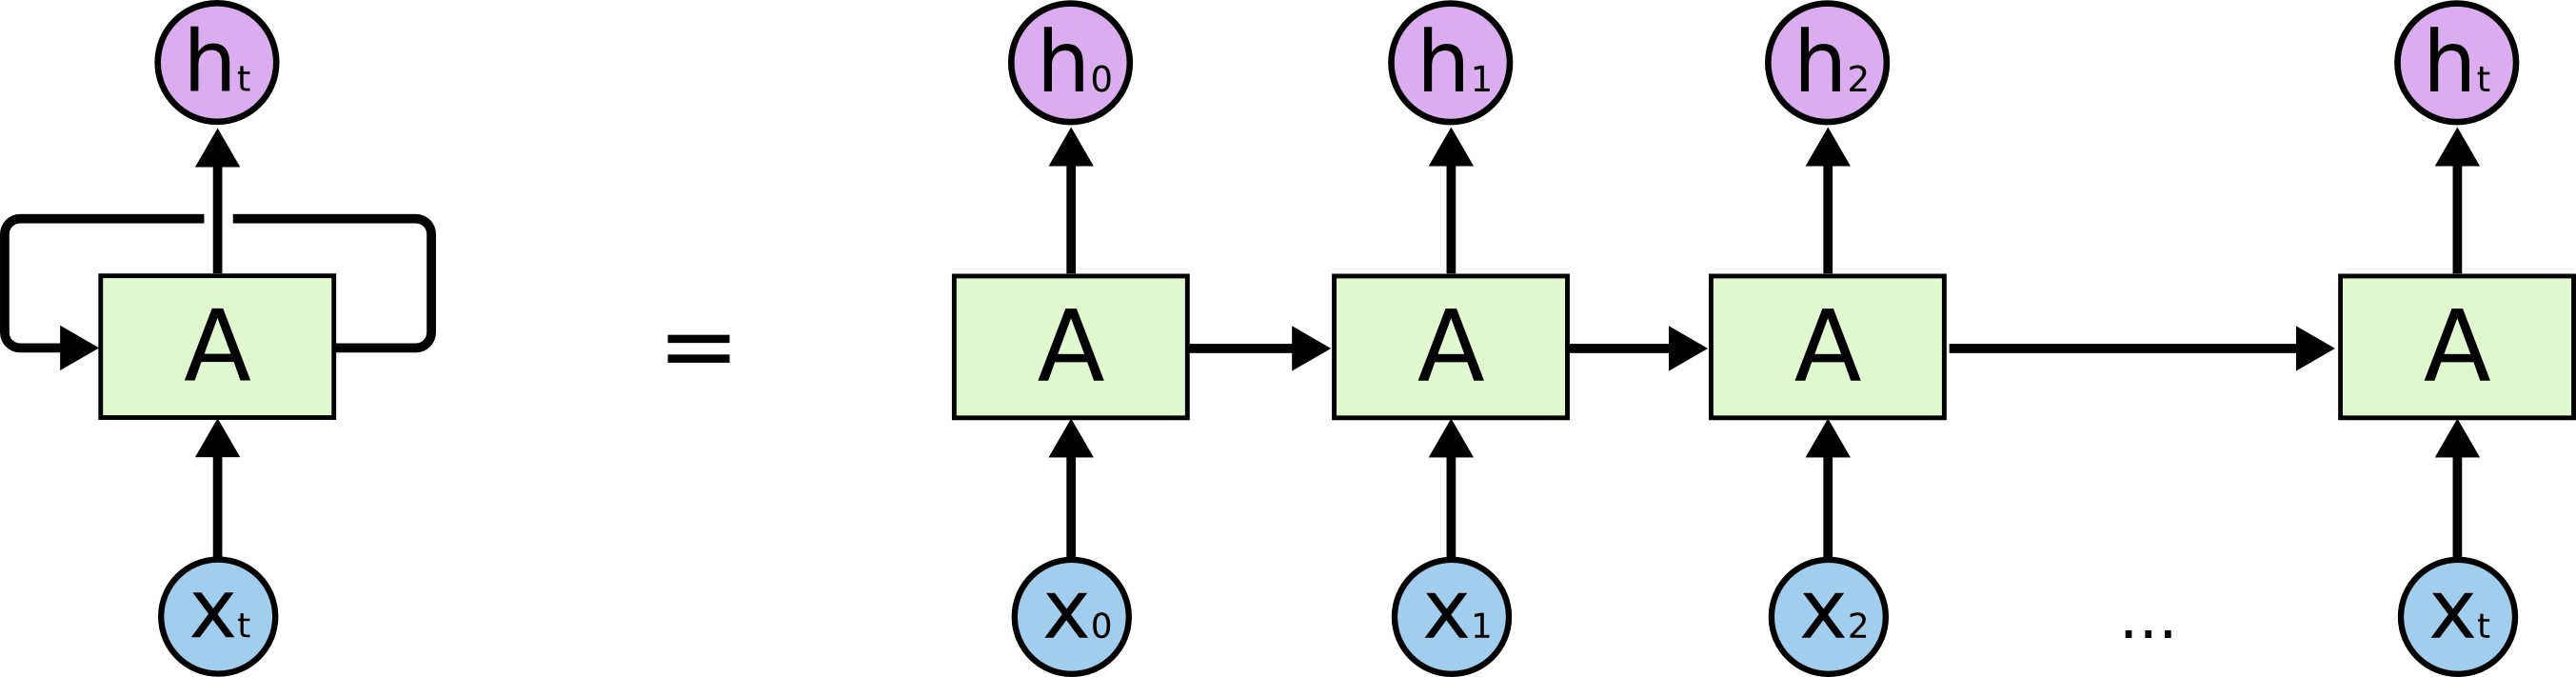
\includegraphics[width=\linewidth]{imgs/rnn_colah_unrolled.png}
\end{center}
\vspace{-15pt}
\captionof{figure}{Unrolled view of Recurrent Neural Network with Hidden States $h_i$ and inputs $x_i$. From \emph{Understanding LSTMs}, by Colah., 2015. \url{https://colah.github.io/posts/2015-08-Understanding-LSTMs/}. Copyright 2015 by Colah.}
%\vspace{15pt}
\label{fig:rnnUnrolledView}
\end{wrapfigure}


Traditional neural networks cannot persist information. As a comparison, while humans do not start thinking from scratch each time they learn something new, neural networks lack memory. Inherently related to sequences, recurrent neural networks use a recurrence or looping mechanism to introduce data persistence in the model to overcome this problem (Colah, 2015). This looping mechanism acts like a ``highway" to flow from one step to the next by passing inputs and modified hidden states along until computing a final prediction (Nguyen, 2018a). 

}



\subsubsection{Describing RNNs}

An RNN is a unidirectional \hyperref[sec:LanguageModels]{language model} since it uses context words left of the target word. It is a neural network that takes in a sequence (sentence) of input symbols (words) $\overrightarrow{x} = \{ x_1, ..., x_T\}$, and for each time $t$, the current hidden state $h_t$ is updated via the formula $h_t = f \Big( h_{t-1}, x_t \Big)$ where $f(\cdot)$ is a nonlinear activation function. The RNN's intermediate task is to predict a probability distribution over an input sequence (sentence) by predicting the next word symbol $x_t$ in the sequence sentence, using left context, so the output at time $t$ is the conditional distribution $P \Big(x_t \; | \; x_{t-1}, ..., x_1 \Big)$. The probability of the entire sequence sentence $\overrightarrow{x}$ is the product of all the probabilities of the individual words, $P(\overrightarrow{x}) = \prod_{t=1}^T P \Big(x_t \; | \; x_{t-1}, ..., x_1 \Big)$ (Cho, 2014). 


    
\subsection{Long-Short Term Memory Networks (LSTM)} \label{sec:LSTM}

\subsubsection{Motivation for LSTM: Vanishing Gradient Problem} \label{sec:ProblemWithRNNs}


{
\begin{wrapfigure}{L}{0.6\textwidth}
\begin{center}
    \vspace{-20pt}
    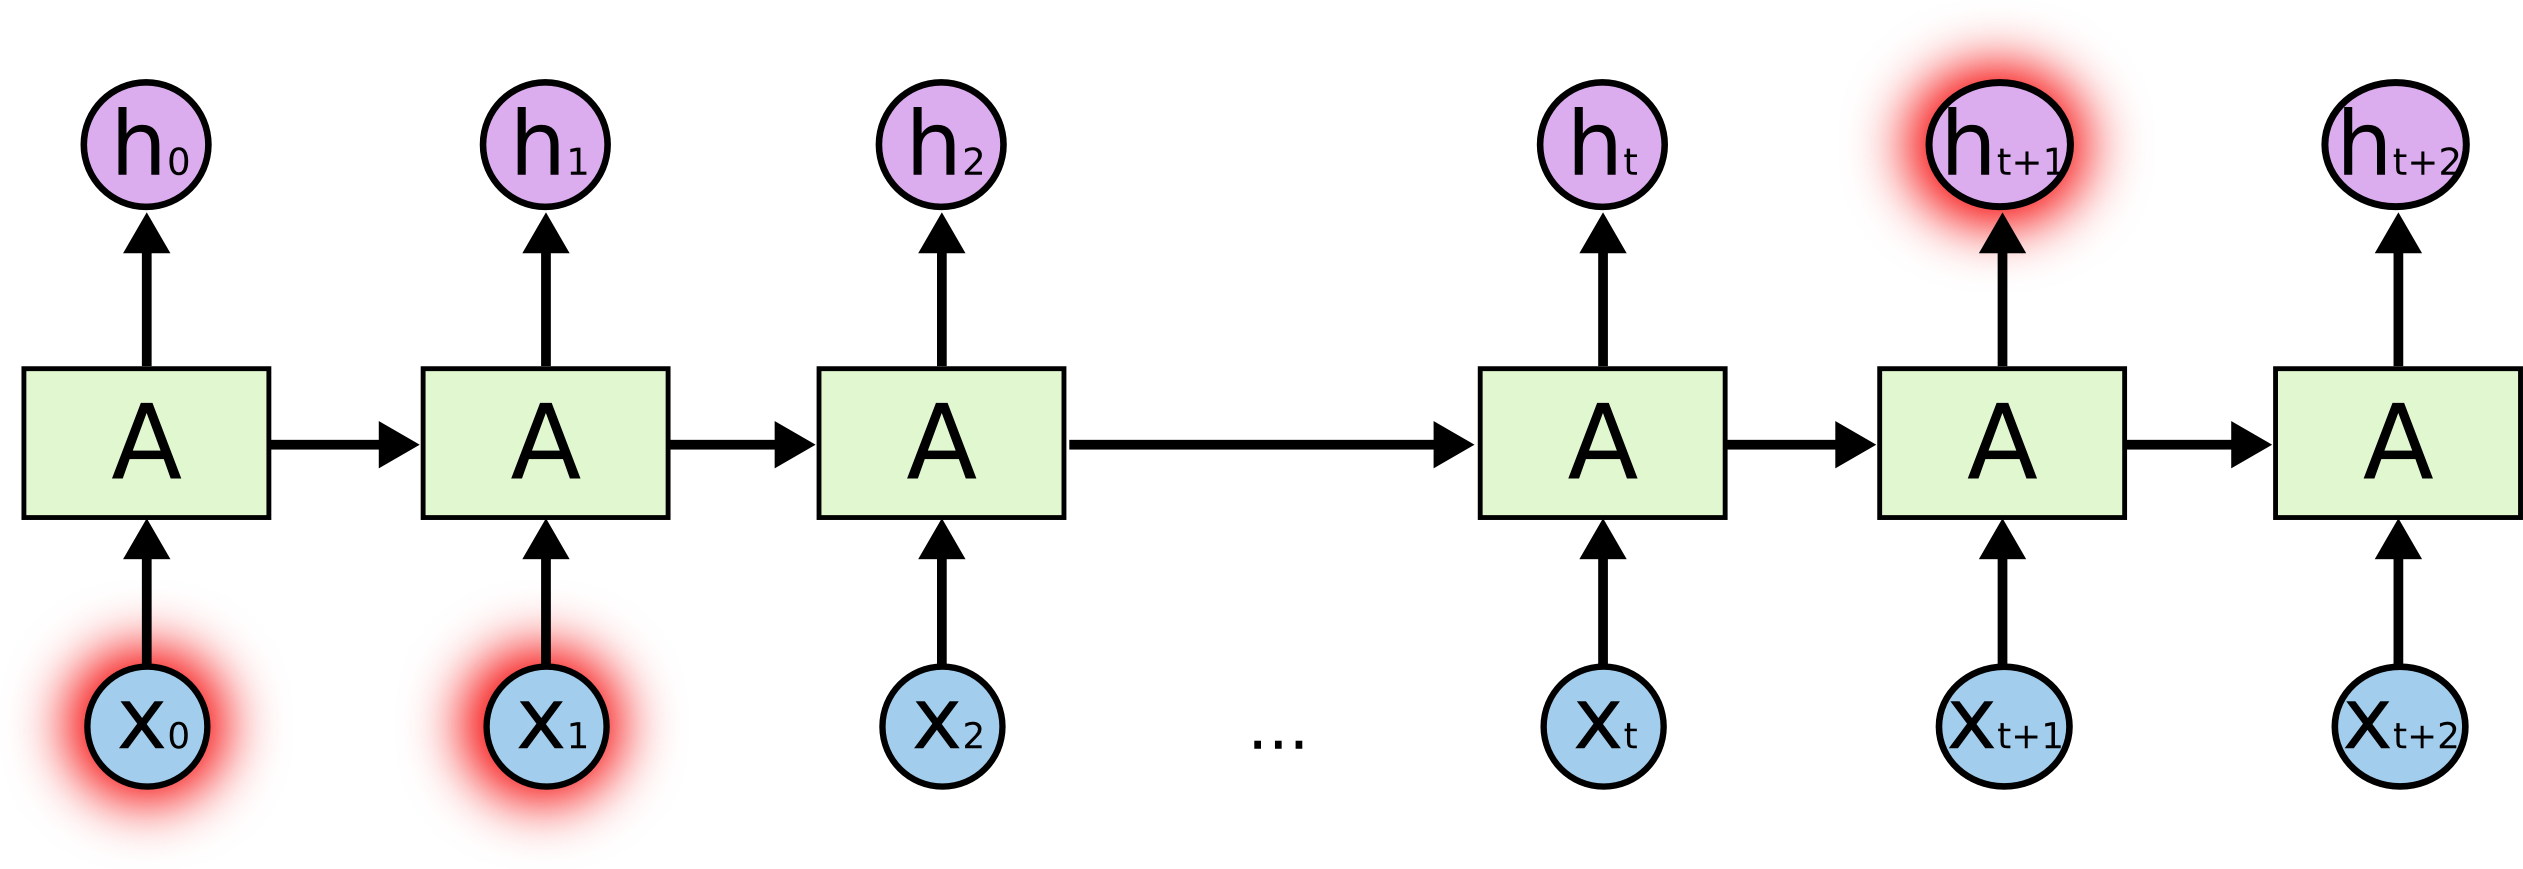
\includegraphics[width=\linewidth]{imgs/rnn_longterm.png}
\end{center}
\vspace{-15pt}
\captionof{figure}{Long-Term Dependency Problem in RNNs (widening gap between inputs $x_i$ and hidden states $h_j$. From \emph{Understanding LSTMs}, by Colah, 2015. \url{https://colah.github.io/posts/2015-08-Understanding-LSTMs/}. Copyright 2015 by Colah.}
%\vspace{15pt}
\label{fig:longTermMemoryProblem}
\end{wrapfigure}


\hyperref[sec:RNN]{RNN}s suffer from the well known \textbf{long-term dependency problem}. In some prediction tasks, longer context is needed to predict a target word. For instance to predict the last word in the sentence ``I grew up in France ... I speak fluent \emph{French}", a model would need the earlier context word ``France." When this gap between target and context words becomes too large, \hyperref[sec:RNN]{RNN}s cannot learn their relationship (Colah, 2015). 

Mathematically speaking, this is due to the \textbf{vanishing gradient problem}. During backward propagation of errors through the \hyperref[sec:RNN]{RNN}, the gradient shrinks as it back propagates through time and becomes too small to update the parameter weights significantly. 


}

This is compounded by the fact that since inputs at any timestep $t$ are dependent on previous $t-1$ outputs, longer sequences require more gradient calculations. Adjustments to earlier layers thus become smaller, causing gradients to shrink exponentially as they are backpropagated through to earlier layers of the \hyperref[sec:RNN]{RNN}. As a result, \hyperref[sec:RNN]{RNN}s ``forget" older history, resulting in short-term memory as shown in \cref{fig:longTermMemoryProblem} (Nguyen, 2018b). 



\subsubsection{Describing LSTMs}

A \textbf{long-short term memory network (LSTM)} is a type of \hyperref[sec:RNN]{RNN} that learns long-term dependencies by design, unlike \hyperref[sec:RNN]{RNN}s. LSTMs use gates or \hyperref[sec:NeuralLM]{neural network}s that decide how to add or remove information from the cell state, explicitly letting the LSTM ``remember" or ``forget" (Nguyen, 2018b). Since LSTMs can accumulate increasingly richer information while parsing the sentence, by the time the last word is reached, the hidden layer of the network provides a \textbf{semantic representation} of the entire sentence (Palangi et al., 2016). 

A core idea in an LSTM is the \textbf{cell state}, shown in \cref{fig:cellState} as the topmost line with the gates merging into it. For example, for a language predicting the next word based on previous ones, the appropriate behavior of its cell state might be to include the gender of the present subject so the model uses correct pronouns. When a new subject is observed, the cell state should forget the old subject's gender and retain the new one (Colah, 2015). 

From Nguyen (2018b), these gates regulate information flow as follows: 


% -------------------------------------------
% Start of the gates
\clearpage



%%% The forget gate image wrapping ---------------------
\begin{program}
\begin{wrapfigure}{L}{0.4\textwidth} 
\begin{center}
    \vspace{-30pt}
    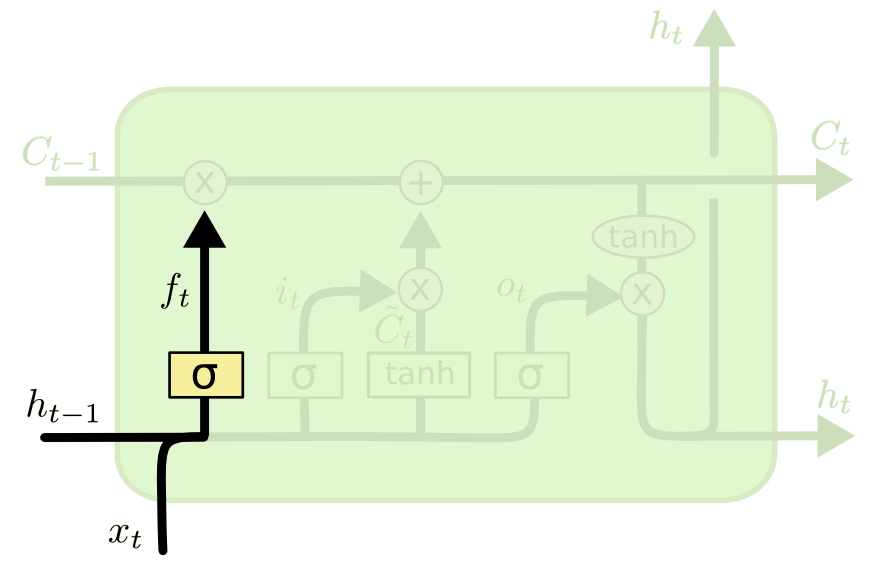
\includegraphics[width=0.9\linewidth]{imgs/lstm_forgetGate.png}
\end{center}
\captionof{figure}{ Forget Gate Calculation. From \emph{Understanding LSTMs}, by Colah, 2015. \url{https://colah.github.io/posts/2015-08-Understanding-LSTMs/}. Copyright 2015 by Colah.}
\label{fig:forgetGate}
\end{wrapfigure}

\ContentFontSize

\textbf{Forget Gate: } the forget gate, shown in \cref{fig:forgetGate}, decides information to discard or keep. The previous hidden state $h_{t-1}$ and current input $x_t$ are passed through the sigmoid nonlinearity function. The forget gate outputs a number between $0$ and $1$ for each number in the cell state $C_{t-1}$; values closer to $0$ indicate the forget gate should discard the information and values closer to $1$ should be kept. 

\begin{equation}
f_t = \sigma \Big( W_f \cdot [h_{t-1}, x_t] + b_f \Big)
\end{equation} 

where $f_t =$ forget gate for time $t$, $\sigma(\cdot) =$ sigmoid, $W_f =$ the weight matrix at the forget layer, and $b_f =$ forget gate's bias term. 

\end{program}



%%% The input gate image wrapping ---------------------
\begin{program}
\begin{wrapfigure}{L}{0.4\textwidth}
\begin{center}
    \vspace{-30pt}
    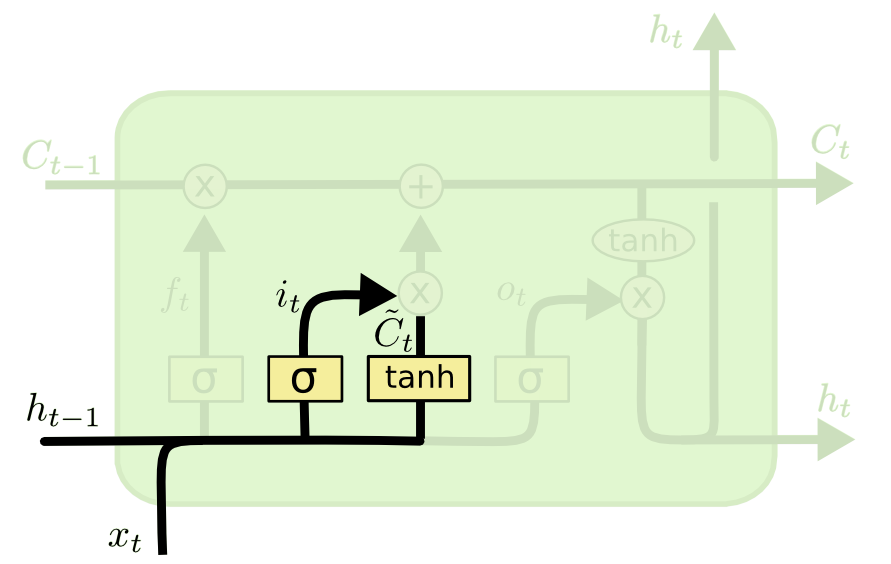
\includegraphics[width=0.9\linewidth]{imgs/lstm_inputGate.png}
\end{center}
\captionof{figure}{ Input Gate Calculation. From \emph{Understanding LSTMs}, by Colah, 2015. \url{https://colah.github.io/posts/2015-08-Understanding-LSTMs/}. Copyright 2015 by Colah.} 
\label{fig:inputGate}
\end{wrapfigure}

\ContentFontSize

\textbf{Input Gate: } the input gate $i_t$, shown in \cref{fig:inputGate}, updates the cell state $C_t$. Previous hidden state $h_{t-1}$ and current input $x_t$ are passed though a signmoid function normalize vector cells between $0$ and $1$. The input gate is later used with the cell state to decide how values are updated. 

\begin{equation}
i_t = \sigma \Big( W_i \cdot [h_{t-1}, x_t] + b_i \Big)
\end{equation}

where $i_t$ is the input gate for time $t$, $\sigma(\cdot)$ is the sigmoid, $W_i$ is the weight matrix at the input layer, and $b_i$ is the input gate's bias term. \par \kern 5pt
\end{program}





%%% The cell state gate image wrapping ---------------------
\begin{program}

\begin{wrapfigure}{L}{0.4\textwidth}
\begin{center}
    \vspace{-30pt}
    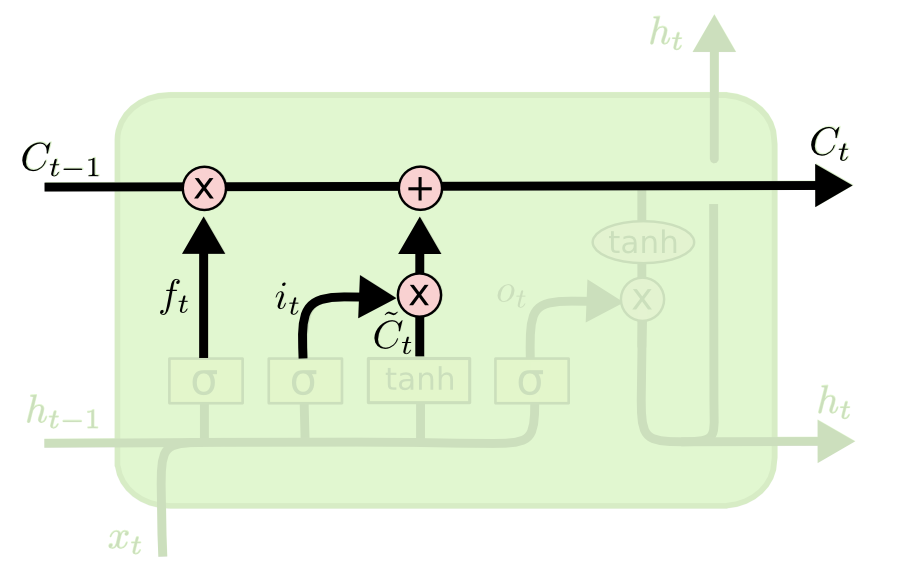
\includegraphics[width=0.9\linewidth]{lstm_cellState.png}    
\end{center}
%\vspace{-25pt}
\captionof{figure}{ Cell State Calculation. From \emph{Understanding LSTMs}, by Colah, 2015.\url{https://colah.github.io/posts/2015-08-Understanding-LSTMs/}. Copyright 2015 by Colah.}
\label{fig:cellState}
\end{wrapfigure}

\ContentFontSize

\textbf{Cell State: } Current cell state $C_t$, shown in \cref{fig:cellState}, takes $h_{t-1}$ and $x_t$ and normalizes them to be between $-1$ and $1$ via a hyperbolic tangent nonlinearity:

\begin{equation}
C_t = \tanh \Big( W_C \cdot [h_{t-1}, x_t] + b_C \Big)
\end{equation}

where $C_t$ is the cell state for time $t$, $\tanh(\cdot)$ is the hyperbolic tangent, $W_C$ is the weight matrix at the cell state layer, and $b_C$ is the cell state's bias term. Next, pointwise multiplications occur to regulate memory in LSTM: 

\begin{equation}
C_t = f_t \cdot C_{t-1} + i_t \cdot C_t
\end{equation}

\end{program}




%%% The output gate image wrapping ---------------------
\begin{program}
\begin{wrapfigure}{L}{0.4\textwidth}
\begin{center}
    \vspace{-30pt}
    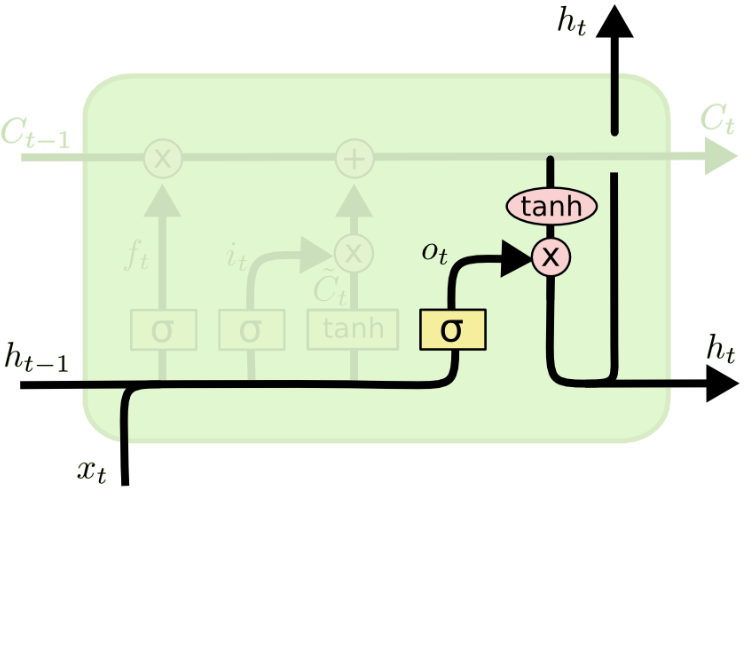
\includegraphics[width=0.27\textwidth]{imgs/lstm_outputGate.png}    
\end{center}
\captionof{figure}{Output Gate Calculation. From \emph{Understanding LSTMs}, by Colah, 2015.\url{https://colah.github.io/posts/2015-08-Understanding-LSTMs/}. Copyright 2015 by Colah.}
\label{fig:outputGate}
\end{wrapfigure}

\ContentFontSize

\textbf{Output Gate: }the output gate, shown in \cref{fig:outputGate}, determines the next hidden state by multiplying the previous output state by the cell state that is filtered by the hyperbolic tangent.

\begin{equation}
\begin{array}{ll}
o_t = \sigma \Big( W_o \cdot [h_{t-1}, x_t] + b_o \Big) \\
h_t = o_t \cdot \tanh(C_t)
\end{array}
\end{equation}

\end{program}


% End of the gates
\clearpage
% -------------------------------------------


\subsection{Gated Recurrent Networks (GRU)} \label{sec:GRU}

The gated recurrent unit (GRU) from Cho et al. (2014) is a type of LSTM that ``combines the forget and input gates into a single \textbf{update gate}" and ``merges the cell state and hidden state" (Colah, 2015), resulting with only the reset gate $r_t$ and update gate $z_t$ (Nguyen, 2018b). 

The \textbf{update gate} $z_t$ controls how much information from previous hidden state contributes to current hidden state, acting like a memory cell in the LSTM to remember long-term dependencies (Cho et al., 2014). 

The \textbf{reset gate} $r_t$ signals the hidden state on how to forget previous information. When the reset gate is close to $0$, the initialized hidden state $\Tilde{h}_t$ must ignore previous hidden state $h_{t-1}$ and reset with the current input $x_t$ only. Intuitively, this allows the activation hidden state $h_t$ to forget any irrelevant information for the future (Cho et al., 2014). 

\begin{figure}[h]
\vspace{-5pt}
\centering
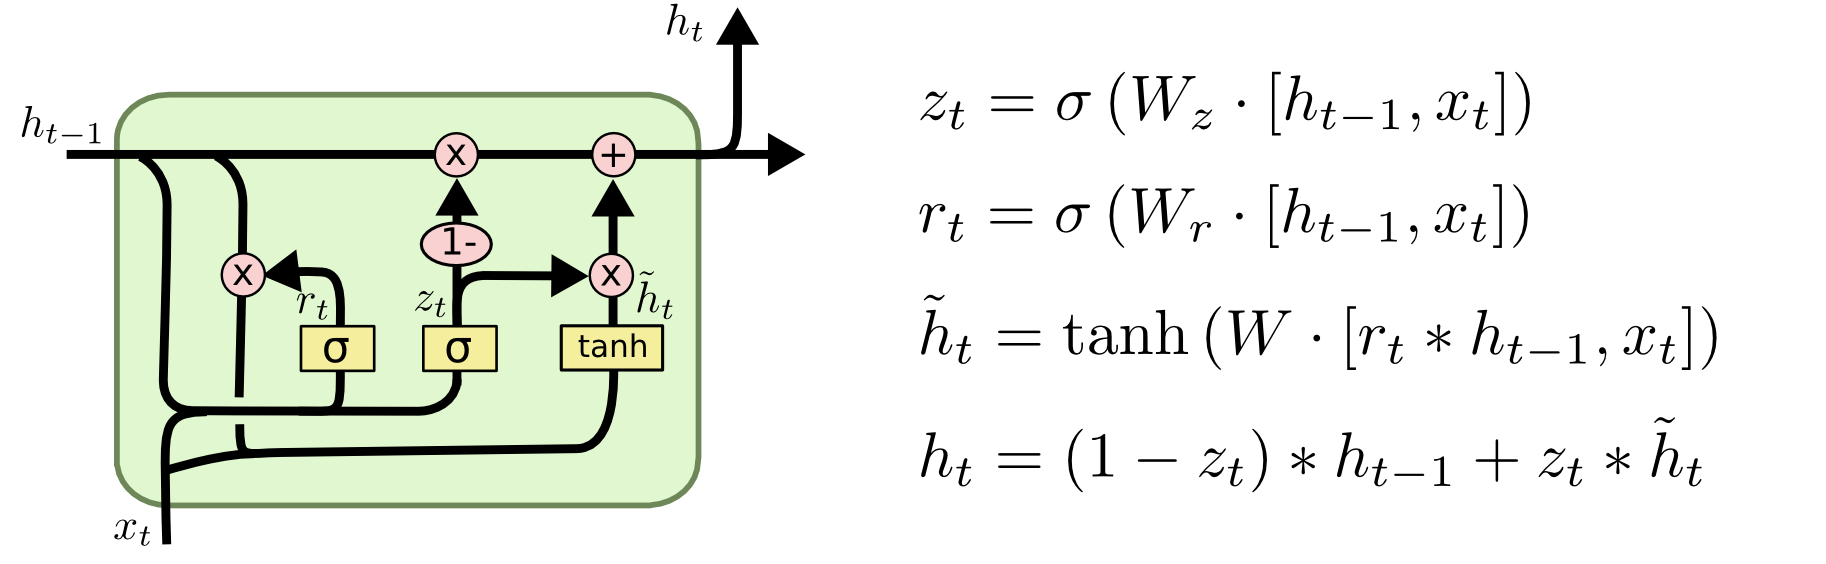
\includegraphics[width=0.8\textwidth]{imgs/gru_withformula.png}
\vspace{-5pt}
\caption{\footnotesize The GRU Cell with Gates. From \emph{Understanding LSTMs}, by Colah, 2015. \url{https://colah.github.io/posts/2015-08-Understanding-LSTMs/}. Copyright 2015 by Colah.}
\vspace{-5pt}
\label{fig:gru}
\end{figure}

Nguyen (2018b) notes that since GRU's have fewer tensor operations, they are more efficient than LSTMs during training. 
The GRU adaptively remembers and forgets because each hidden unit has separate reset and update gates so each hidden unit can capture dependencies over different time scales. Frequently active reset gates help the GRU remember short-term dependencies while frequently active update gates help the GRU note long-term dependencies (Cho et al., 2014). 


%\clearpage
%\section{APPENDIX: Application To Machine Translation in NLP (Using PyTorch and Skip-Gram)}\label{app:Appendix_SkipGram}



Author: Ana-Maria Vintila, based off work from Srijith Rajamohan based
off the work by Robert Guthrie

Source: https://srijithr.gitlab.io/post/word2vec/

\begin{verbatim}
import os
from IPython.display import Image

pth = os.getcwd()
pth
\end{verbatim}

\begin{verbatim}
'/content/gdrive/My Drive/StatFitScholarshipProject/PythonNeuralNetNLP'
\end{verbatim}

\begin{verbatim}
Image(filename=pth + '/src/NLPstudy/images/Skip-gram.png')
\end{verbatim}

\begin{figure}
\centering
\includegraphics{SkipGram_Rajamohan_files/SkipGram_Rajamohan_3_0.png}
\caption{png}
\end{figure}

Loading the imports:

\begin{verbatim}
import torch
import torch.tensor as Tensor
import torch.nn as nn
import torch.nn.functional as F
import torch.optim as optim
import numpy as np
import urllib.request
from nltk.tokenize import RegexpTokenizer
from nltk.corpus import stopwords
from nltk import word_tokenize
import sklearn
from sklearn.cluster import KMeans
from sklearn.metrics.pairwise import euclidean_distances

torch.manual_seed(1)
\end{verbatim}

\begin{verbatim}
<torch._C.Generator at 0x7f9c3be47370>
\end{verbatim}

\hypertarget{step-1-initialization}{%
\section{Step 1: Initialization}\label{step-1-initialization}}

Here we set the context window size to \(3\) words and the word
embedding dimension to \(10\), and also pass in the text corpora from
which we build vocabulary.

Tokenizing the text occurs later while reading in the data.

\begin{verbatim}
CONTEXT_SIZE = 3
EMBEDDING_DIM = 10

testSentence = """Empathy for the poor may not come easily to people who never experienced it.
They may blame the victims and insist their predicament can be overcome through determination
and hard work.
But they may not realize that extreme poverty can be psychologically and physically
incapacitating — a perpetual cycle of bad diets, health care and education exacerbated
by the shaming and self-fulfilling prophecies that define it in the public imagination.
Gordon Parks — perhaps more than any artist — saw poverty as “the most savage of all human
afflictions” and realized the power of empathy to help us understand it. It was neither an
abstract problem nor political symbol, but something he endured growing up destitute in rural
Kansas and having spent years documenting poverty throughout the world, including the United
States.
That sensitivity informed “Freedom’s Fearful Foe: Poverty,” his celebrated photo essay published
 in Life magazine in June 1961. He took readers into the lives of a Brazilian boy, Flavio
 da Silva, and his family, who lived in the ramshackle Catacumba favela in the hills outside
 Rio de Janeiro. These stark photographs are the subject of a new book, “Gordon Parks: The
  Flavio Story” (Steidl/The Gordon Parks Foundation), which accompanies a traveling exhibition
  co-organized by the Ryerson Image Centre in Toronto, where it opens this week, and
  the J. Paul Getty Museum. Edited with texts by the exhibition’s co-curators, Paul Roth and
  Amanda Maddox, the book also includes a recent interview with Mr. da Silva and essays by
  Beatriz Jaguaribe, Maria Alice Rezende de Carvalho and Sérgio Burgi.
""".split()
\end{verbatim}

\hypertarget{step-2-build-the-n-grams}{%
\section{\texorpdfstring{Step 2: Build the
\(n\)-grams}{Step 2: Build the n-grams}}\label{step-2-build-the-n-grams}}

Next we build the \(n\)-grams, or sequence of words, as a list of
tuples.

Each tuple is ({[} \texttt{word}\(_{i-2}\), \texttt{word}\(_{i-1}\) {]},
\texttt{targetWord})

\begin{verbatim}
ngrams = []
for i in range(len(testSentence) - CONTEXT_SIZE):
    tup = [testSentence[j] for j in np.arange(i + 1, i + CONTEXT_SIZE + 1)]
    # skip-gram way of appending:
    ngrams.append( (testSentence[i], tup) )
    # cbow# ngrams.append( (tup, testSentence[i + CONTEXT_SIZE]) )
\end{verbatim}

\begin{verbatim}
ngrams[:20] # showing a few sample n-grams
\end{verbatim}

\begin{verbatim}
[('Empathy', ['for', 'the', 'poor']),
 ('for', ['the', 'poor', 'may']),
 ('the', ['poor', 'may', 'not']),
 ('poor', ['may', 'not', 'come']),
 ('may', ['not', 'come', 'easily']),
 ('not', ['come', 'easily', 'to']),
 ('come', ['easily', 'to', 'people']),
 ('easily', ['to', 'people', 'who']),
 ('to', ['people', 'who', 'never']),
 ('people', ['who', 'never', 'experienced']),
 ('who', ['never', 'experienced', 'it.']),
 ('never', ['experienced', 'it.', 'They']),
 ('experienced', ['it.', 'They', 'may']),
 ('it.', ['They', 'may', 'blame']),
 ('They', ['may', 'blame', 'the']),
 ('may', ['blame', 'the', 'victims']),
 ('blame', ['the', 'victims', 'and']),
 ('the', ['victims', 'and', 'insist']),
 ('victims', ['and', 'insist', 'their']),
 ('and', ['insist', 'their', 'predicament'])]
\end{verbatim}

\hypertarget{step-3-create-vocabulary}{%
\section{Step 3: Create Vocabulary}\label{step-3-create-vocabulary}}

Create the vocabulary by converting the text into a \texttt{set} to
remove duplicate words.

\begin{verbatim}
vocabulary = set(testSentence)
\end{verbatim}

\begin{verbatim}
len(vocabulary)
list(vocabulary)[:20] # showing first 20 words in vocabulary
\end{verbatim}

\begin{verbatim}
['lived',
 'psychologically',
 'prophecies',
 'Gordon',
 'Silva',
 'They',
 'abstract',
 'perpetual',
 'hills',
 'Silva,',
 'power',
 'magazine',
 'imagination.',
 'something',
 'recent',
 'all',
 'may',
 'understand',
 'cycle',
 'who']
\end{verbatim}

\hypertarget{step-4-create-map-of-words-to-indices}{%
\section{Step 4: Create Map of Words to
Indices}\label{step-4-create-map-of-words-to-indices}}

Creating word to index map that prints the key (word) corresponding to
the given index in the dictionary argument. Basically, we get a list of
tuples (number, word) from zipping the sequence \(0,1,2,3 ....\) with
the vocabulary word list.

\begin{verbatim}
wordToIndex = {word : i for i, word in enumerate(vocabulary)}
\end{verbatim}

\begin{verbatim}
# Showing first 20 word to index pairs
len(wordToIndex)
itemsList = list(wordToIndex.items())
itemsList[:20]
\end{verbatim}

\begin{verbatim}
[('lived', 0),
 ('psychologically', 1),
 ('prophecies', 2),
 ('Gordon', 3),
 ('Silva', 4),
 ('They', 5),
 ('abstract', 6),
 ('perpetual', 7),
 ('hills', 8),
 ('Silva,', 9),
 ('power', 10),
 ('magazine', 11),
 ('imagination.', 12),
 ('something', 13),
 ('recent', 14),
 ('all', 15),
 ('may', 16),
 ('understand', 17),
 ('cycle', 18),
 ('who', 19)]
\end{verbatim}

\begin{verbatim}
def printKey(iWord, wordToIndexDict):
    """
    Prints the key (the word) corresponding to the given index in the given dictionary.

    :param iWord: index of a word in the given dict
    :param wordToIndexDict: the dictionary
    :return: key
    """
    for key, index in wordToIndexDict.items():
        if(index == iWord):
            print(key)



def clusterEmbeddings(filename, numClusters):
    X = np.load(filename)
    kmeans = KMeans(n_clusters=numClusters, random_state=  0).fit(X) # from sklearn
    center = kmeans.cluster_centers_
    distances = euclidean_distances(X, center)

    for i in np.arange(0, distances.shape[1]):

        # get the index of the minimum distance in the ith row of the dist matrix
        iMinWord = np.argmin(distances[:, i])
        print(iMinWord)
        printKey(iWord=iMinWord, wordToIndexDict= wordToIndex)


def readData(filePath):
    tokenizer = RegexpTokenizer(r'\w+')
    data = urllib.request.urlopen(filePath)
    data = data.read().decode('utf8')
    tokenizedData = word_tokenize(data)

    # note: stopwords are from nltk
    stopWordsSet = set(stopwords.words('english'))
    stopWordsSet.update(['.',',',':',';','(',')','#','--','...','"'])
    cleanedWords = [word for word in tokenizedData if word not in stopWordsSet]

    return cleanedWords
\end{verbatim}

\hypertarget{step-6-create-skip-gram-model}{%
\section{Step 6: Create Skip-Gram
Model}\label{step-6-create-skip-gram-model}}

The skip-gram neural network has three components:

\begin{enumerate}
\def\labelenumi{\arabic{enumi}.}
\tightlist
\item
  embedding layer, created using pytorch's \texttt{nn.Embedding}, to
  convert tensors into word embeddings.
\item
  hidden layer, in this case it is a linear layer.
\item
  output layer, in this case also linear layer.
\end{enumerate}

\hypertarget{forward-pass-of-skip-gram}{%
\subsubsection{Forward Pass of
Skip-Gram:}\label{forward-pass-of-skip-gram}}

\begin{enumerate}
\def\labelenumi{\arabic{enumi}.}
\tightlist
\item
  Convert the tensor \texttt{inputs} to word embeddings via the
  skip-gram's \texttt{nn.Embedding} layer
\item
  Pass the embeddings to the hidden layer and transform the result using
  the \texttt{relu} function
\item
  Transform the hidden layer results using the output layer.
\item
  Finally, create a probability distribution over words using the
  \texttt{softmax} function. (Here we actually use the
  \texttt{log\_softmax} so the results are log probabilities instead of
  probabilities. )
\end{enumerate}

\hypertarget{predictions}{%
\subsubsection{Predictions:}\label{predictions}}

To generate predictions we need to execute the \texttt{forward} pass of
the skip-gram model and get the index of the maximum probability from
the output layer. Then that index is used to find the corresponding
prediction word.

\begin{verbatim}
class SkipGramModeler(nn.Module):

    def __init__(self, vocabSize: int, embeddingDim: int, contextSize: int):
        super(SkipGramModeler, self).__init__()

        # see docs: https://hyp.is/cv2pSAeqEeqIRHv7JAjgtA/pytorch.org/docs/stable/nn.html
        # num_embeddings = size of the dictionary embeddings
        # embedding_dim = the size of each embedding vector
        # Creating an embedding model that contains (vocabSize) tensors each of size (embeddingDim)
        self.embeddings = nn.Embedding(num_embeddings=vocabSize,
                                       embedding_dim=embeddingDim,
                                       padding_idx=contextSize)

        # see nn.Linear docs
        # https://hyp.is/XEDPhgerEeqFhHssJYoa-w/pytorch.org/docs/stable/nn.html
        # note: in_features = size of each input sample
        # note: out_features = size of each output sample
        self.hiddenLayer = nn.Linear(in_features=embeddingDim,
                                     out_features=128)

        self.outputLayer = nn.Linear(in_features=128,
                                     out_features=contextSize * vocabSize)


    def forward(self, inputs: Tensor) -> Tensor:
        """

        :param inputs: 1-dim tensor
        :return:
        """
        # note: -1 implies the size inferred for that index from the size of data
        # is a tensor
        inputEmbeddings: Tensor = self.embeddings(inputs).view((1,-1))

        # output at hidden layer
        hiddenRELUResults: Tensor = F.relu(self.hiddenLayer(inputEmbeddings))
        # output at final layer
        outputResults: Tensor = self.outputLayer(hiddenRELUResults)

        logProbs: Tensor = F.log_softmax(input=outputResults, dim=1).view(CONTEXT_SIZE, -1)

        return logProbs



    def predict(self, inputStr: str, wordToIndexDict: dict) -> list:
        """

        :param inputStr: single word (targetword) from which we predict context list
        :return:
        """
        contextIndices: Tensor = torch.tensor([wordToIndexDict[inputStr]],
                                              dtype=torch.long)

        logProbs: Tensor = self.forward(contextIndices)

        # get index of maximum log probability from output layer
        #iMaxLogProbs: Tensor = torch.argmax(logProbs)

        # returns log probs sorted in descending order and
        # iSorted = indices of elements in the input tensor
        logProbsDecr, iSorted = logProbs.sort(descending=True)

        # same as logs.squeeze()[:3] (erasing first dimension)
        # since the tensor is [[...]]

        # getting sorted indices, the first one in each row of iSorted
        # (there are three rows in the iSorted, 2-dim tensor)
        numRows, numCols = iSorted.size()
        iFirstCol = 0
        indices = [iSorted[r][iFirstCol] for r in np.arange(0, numRows)]


        keyIndFilteredPairs: list = []

        for i in indices:

            keyIndFilteredPairs.append( [ (key, index)
                                       for key, index in wordToIndexDict.items()
                                       if index == i ]  )

        return keyIndFilteredPairs

    def printLayerParamers(self):
        for name, child in self.named_children():
            print("\nname = {}, child = {}".format(name, child))

            # TODO: type of child?
            for names, params in child.named_parameters():
                print("names = {}, params = {}".format(names, params))
                print("params.size() = {}".format(params.size()))


    def writeEmbeddingToFile(self, filename: str):
        for i in self.embeddings.parameters():
            weights = i.data.numpy()
        np.save(filename, weights)
\end{verbatim}

\begin{verbatim}
# Trial : testing out the predict() inner workings

inputStr = "psychologically"

contextIndices: Tensor = torch.tensor([wordToIndex[inputStr]],
                                      dtype=torch.long)
print("contextIndices: ", contextIndices)
print("contextIndices dim: ", contextIndices.dim())
print("contextIndices size: ", contextIndices.size())

\end{verbatim}

\begin{verbatim}
contextIndices:  tensor([137])
contextIndices dim:  1
contextIndices size:  torch.Size([1])
\end{verbatim}

\begin{verbatim}
dummyModel = SkipGramModeler(vocabSize=len(vocabulary), embeddingDim=EMBEDDING_DIM,
                         contextSize=CONTEXT_SIZE)

logProbs: Tensor = dummyModel(contextIndices)


# returns log probs sorted in descending order and
# iSorted = indices of elements in the input tensor
logProbsDecr, iSorted = logProbs.sort(descending=True)
print("logProbsDecr dim : ", logProbsDecr.dim())
print("logProbsDecr shape : ", logProbsDecr.shape)
print("logProbsDecr squeezed: ", logProbsDecr.squeeze()[:, :5])
print("logProbsDecr squeezed dim :  ", logProbsDecr.squeeze().dim())
print("logProbsDecr squeezed shape: ", logProbsDecr.squeeze().shape)

print("\niSorted dim: ", iSorted.dim())
# note: in this case, squeezing is same as the original tensor; has no effect
print("iSorted: ", iSorted[:, :5])

logProbsDecr = logProbsDecr.squeeze()   # logProbsDecr[0][:3]
iSorted = iSorted.squeeze()



# getting sorted indices, the first one in each row of iSorted
# (there are three rows in the iSorted, 2-dim tensor)
numRows, numCols = iSorted.size()
iFirstCol = 0
indices = [iSorted[r][iFirstCol] for r in np.arange(0, numRows)]

print("\nindices = ", indices)


# it length will be numRows of iSorted (numRows = 3)
# which equals CONTEXT_SIZE
keyIndFilteredPairs: list = []

for i in indices:

    keyIndFilteredPairs.append( [ (key, index)
                                  for key, index in wordToIndex.items()
                                  if index == i ]  )

print("\nlength of key,ind pairs: ", len(keyIndFilteredPairs))
print("keyIndFilteredPairs: ", keyIndFilteredPairs)
\end{verbatim}

\begin{verbatim}
logProbsDecr dim :  2
logProbsDecr shape :  torch.Size([3, 195])
logProbsDecr squeezed:  tensor([[-5.7581, -5.7919, -5.8080, -5.8146, -5.8202],
        [-5.5920, -5.6021, -5.6844, -5.7157, -5.7189],
        [-5.6294, -5.6362, -5.6638, -5.6691, -5.7091]],
       grad_fn=<SliceBackward>)
logProbsDecr squeezed dim :   2
logProbsDecr squeezed shape:  torch.Size([3, 195])

iSorted dim:  2
iSorted:  tensor([[107,  95,  74,  63,  11],
        [142, 106, 100,  10,  93],
        [167,   1,  44,   9,   8]])

indices =  [tensor(107), tensor(142), tensor(167)]

length of key,ind pairs:  3
keyIndFilteredPairs:  [[('traveling', 107)], [('outside', 142)], [('Foundation),', 167)]]
\end{verbatim}

\hypertarget{step-7-train-the-skip-gram-model}{%
\section{Step 7: Train the Skip-Gram
Model}\label{step-7-train-the-skip-gram-model}}

Training the model requires the following steps:

\begin{enumerate}
\def\labelenumi{\arabic{enumi}.}
\tightlist
\item
  Convert the context words into integer indices using the
  \texttt{wordToIndex} dictionary, and make their type a
  \texttt{Tensor}.
\item
  Set the model gradients to zero so they do not accumulate artificially
  (feature of pytorch)
\item
  Do the \texttt{forward} pass of the Skip-Gram model, resulting in the
  log probabilities of the context words.
\item
  For each word in the correct target context wrods, convert it to an
  index using the \texttt{wordToIndex} dictionary and wrap it in a
  \texttt{Tensor} type.
\item
  Compute the loss between the log probabilities and target contexts.
\item
  Do the \texttt{backward} pass over the neural network to update the
  gradients by calling \texttt{loss.backward()}.
\item
  Do one step using the optimizer, so that weights are updated using
  stochastic gradient descent.
\item
  Increment the total loss by this epoch's current loss.
\end{enumerate}

\begin{verbatim}
%time

learningRate = 0.001
NUM_EPOCHS = 550

losses = []
lossFunction = nn.NLLLoss()
skipGramModel = SkipGramModeler(vocabSize = len(vocabulary),
                        embeddingDim=EMBEDDING_DIM,
                        contextSize=CONTEXT_SIZE)
# Using the stochastic-gradient descent optimizer.
optimizer = optim.SGD(skipGramModel.parameters(), lr = learningRate)

# Preserve the data by freezing the embedding layer
#skipGramModel.freezeLayer("embeddingsSkipGram")

for epoch in range(NUM_EPOCHS):
    totalLoss = 0

    # note: skipgram predicts CONTEXT from single word
    # while CBOW predicts single TARGET word from CONTEXT list
    for contextWord, targetContext in ngrams:

        # Step 1: Prepare the inputs to be passed to the model (means
        # turn the words into integer indices and wrap them in tensors)
        contextIndices: Tensor = torch.tensor([wordToIndex[contextWord]],
                                              dtype=torch.long)

        # Step 2:
        skipGramModel.zero_grad()

        # Step 3: run forward pass, getting log probs over the next words
        logProbs = skipGramModel(contextIndices)

        # Step 4: compute loss, where target word is wrapped in a tensor
        targetContextTensor: Tensor = torch.tensor([wordToIndex[w] for w in targetContext],
                                           dtype=torch.long)

        loss = lossFunction(logProbs, targetContextTensor)

        # Step 5: do backward pass and update gradient
        loss.backward()
        optimizer.step()

        totalLoss += loss.item()

    if(epoch % 50 == 0):
        print("Epoch = {}, Total loss = {}".format(epoch, totalLoss))

    losses.append(totalLoss)
\end{verbatim}

\begin{verbatim}
CPU times: user 2 µs, sys: 0 ns, total: 2 µs
Wall time: 4.53 µs
Epoch = 0, Total loss = 1640.9999227523804
Epoch = 50, Total loss = 1518.4927296638489
Epoch = 100, Total loss = 1414.1443753242493
Epoch = 150, Total loss = 1292.492782831192
Epoch = 200, Total loss = 1149.2484674453735
Epoch = 250, Total loss = 998.4024060964584
Epoch = 300, Total loss = 857.8129457235336
Epoch = 350, Total loss = 742.0071568489075
Epoch = 400, Total loss = 655.678228020668
Epoch = 450, Total loss = 594.8056415319443
Epoch = 500, Total loss = 552.3266983032227
\end{verbatim}

\begin{verbatim}
skipGramModel.predict(inputStr = "psychologically", wordToIndexDict=wordToIndex)
skipGramModel.writeEmbeddingToFile(filename = pth + "/src/NLPstudy/SkipGramModel/rajamohan_skipgram_embeddings.txt")
\end{verbatim}

\begin{verbatim}
clusterEmbeddings(filename = pth + "/src/NLPstudy/SkipGramModel/rajamohan_skipgram_embeddings.txt.npy", numClusters=5)
\end{verbatim}

\begin{verbatim}
3
shaming
28
victims
191
It
18
book,
87
Silva,
\end{verbatim}

\begin{verbatim}
\end{verbatim}

%\clearpage
%\section{APPENDIX: Application To Machine Translation in NLP (Using PyTorch and Continuous-Bag-of-Words (CBOW))} \label{app:Appendix_CBOW}


\clearpage
\section{APPENDIX: Application To Machine Translation in NLP (Using PyTorch and Seq-To-Seq Model With Attention)} \label{app:Appendix_Seq2Seq}




%\clearpage
%\input{Appendix_Tutorial_TransformerModel.tex}
%\clearpage
%\input{Appendix_Tutorial_LSTMFromScratch.tex}
% ----------------------------------------------------------------
% Report End

\end{document}